% ============================================================
%  KLTN – Hệ thống phát hiện rò rỉ khí gas thông minh
%  Trường Đại học Công nghệ Thông tin – ĐHQG TP.HCM
% ============================================================
\documentclass{template/thesis}

\Title{HỆ THỐNG PHÁT HIỆN RÒ RỈ KHÍ GAS THÔNG MINH TÍCH HỢP IoT, DỰ BÁO LSTM VÀ HỌC TĂNG CƯỜNG PPO}
\Title[en]{A SMART GAS LEAK DETECTION SYSTEM INTEGRATING IoT, LSTM FORECASTING AND PPO REINFORCEMENT LEARNING}

\ThesisType{KHÓA LUẬN TỐT NGHIỆP}

\University{ĐẠI HỌC QUỐC GIA THÀNH PHỐ HỒ CHÍ MINH}
\CollegeOrDept{{TRƯỜNG ĐẠI HỌC CÔNG NGHỆ THÔNG TIN}}
\Faculty{KHOA MẠNG MÁY TÍNH VÀ TRUYỀN THÔNG}
\Degree{CỬ NHÂN}
\Major{MẠNG MÁY TÍNH VÀ TRUYỀN THÔNG DỮ LIỆU}

\usepackage{amsmath}
\usepackage{graphicx}
\usepackage{float}
\usepackage{placeins}
\usepackage{needspace}
\usepackage{listings}
\usepackage{xcolor}
\usepackage{booktabs}
\usepackage{multirow}
\usepackage{array}
\usepackage{pgfgantt}
\usepackage{enumitem}
\usepackage{longtable}

% Màu sắc cho Gantt chart
\definecolor{primaryblue}{HTML}{2E75B6}
\definecolor{criticalred}{HTML}{C00000}

% Code listing style
\lstset{
  basicstyle=\ttfamily\small,
  keywordstyle=\color{blue}\bfseries,
  commentstyle=\color{gray}\itshape,
  stringstyle=\color{orange},
  numbers=left,
  numberstyle=\tiny\color{gray},
  breaklines=true,
  frame=single,
  captionpos=t,
  aboveskip=1em,
  belowskip=1em,
  tabsize=2,
  showstringspaces=false
}

\graphicspath{{img/}}

\Author{Lê Viết Dương}{22520300}
\Author{Quách Minh Đông}{22520259}

\ThesisYear{2026}
\ThesisLocation{TP. HỒ CHÍ MINH}

\Supervisor{ThS. Nguyễn Khánh Thuật}

\DeclareBibliographyCategory{vietnamese}
\addtocategory{vietnamese}{pccc2023}

\hypersetup{
  pdfencoding=auto,
  pdfauthor={Lê Viết Dương, Quách Minh Đông},
  pdfsubject={Phát hiện rò rỉ khí gas thông minh},
  pdftitle={Hệ thống phát hiện rò rỉ khí gas thông minh tích hợp IoT, dự báo LSTM và học tăng cường PPO},
  pdfkeywords={IoT, LSTM, Reinforcement Learning, Gas Leak Detection, Kafka, Spark, Telegram}
}

\begin{document}

\beforepreface
\afterpreface

\chapter{Mở đầu}
\label{c:intro}
% ============================================================
%  Chương 1: Mở đầu
% ============================================================

Chương mở đầu trình bày bối cảnh hình thành đề tài, nhu cầu phát hiện và ứng phó rò rỉ khí gas trong môi trường nhà ở, cũng như những hạn chế của cách cảnh báo bằng ngưỡng tĩnh. Từ đó, chương này xác định mục tiêu, đóng góp, phạm vi nghiên cứu và cấu trúc của khóa luận. Đây là cơ sở để các chương sau triển khai phần lý thuyết, phương pháp hiện thực và thực nghiệm đánh giá.

\section{Tính cấp thiết của đề tài}

Khí gas hóa lỏng (LPG) và khí tự nhiên (natural gas) được sử dụng rộng rãi trong các hộ gia đình và cơ sở sản xuất tại Việt Nam. Tuy nhiên, đây cũng là nguồn gây ra các vụ cháy nổ nghiêm trọng do rò rỉ không được phát hiện kịp thời. Theo báo cáo của Cục Phòng cháy chữa cháy và Cứu nạn cứu hộ \cite{pccc2023}, hàng năm xảy ra hàng trăm vụ cháy nổ liên quan đến khí gas tại Việt Nam, gây thiệt hại lớn về người và tài sản.

Các hệ thống phát hiện khí gas thương mại hiện tại chủ yếu hoạt động theo nguyên tắc ngưỡng tĩnh: cảm biến đo nồng độ khí theo thời gian thực và kích hoạt cảnh báo khi nồng độ vượt một ngưỡng định sẵn (thường là 10\% LEL – Lower Explosive Limit). Cách làm này đơn giản và dễ triển khai, nhưng vẫn còn một số hạn chế:

\begin{itemize}
  \item Phản ứng muộn: Cảnh báo chỉ phát ra khi khí đã đạt mức nguy hiểm, đúng lúc người dùng có thể đã ngửi thấy mùi. Không còn nhiều thời gian để sơ tán hay can thiệp.
  \item Tỷ lệ cảnh báo sai cao: Các yếu tố môi trường như độ ẩm, nhiệt độ, và sự hiện diện của các khí khác có thể kích hoạt cảnh báo nhầm \cite{tian2019}.
  \item Không có khả năng dự báo: Hệ thống ngưỡng tĩnh không thể phân biệt được một vụ rò rỉ đang tăng dần nguy hiểm (sẽ đạt ngưỡng trong vài phút) với một mức nền cao hơn bình thường nhưng ổn định.
  \item Phản ứng đơn lẻ: Hầu hết chỉ phát âm thanh báo động, không tự động kích hoạt các biện pháp giảm thiểu như bật quạt thông gió hay đóng van gas.
\end{itemize}

Sự phát triển của Internet of Things (IoT) và học máy giúp có thêm hướng xử lý chủ động hơn: hệ thống không chỉ đọc giá trị cảm biến hiện tại mà còn có thể theo dõi xu hướng tăng của khí, ước lượng rủi ro trong vài phút tới và chọn cách can thiệp phù hợp. Đây là hướng mà nhóm lựa chọn để triển khai trong đề tài.

\section{Tổng quan về các nghiên cứu liên quan}

Nhiều nhóm nghiên cứu đã đề xuất các cải tiến cho hệ thống phát hiện khí gas truyền thống.

Hướng tiếp cận cảm biến và IoT: Saranya và cộng sự \cite{saranya2023} xây dựng hệ thống phát hiện khí gas sử dụng Arduino và cảm biến MQ-2, tích hợp cảnh báo qua SMS. Nwazor và cộng sự \cite{nwazor2023} đề xuất kiến trúc IoT dựa trên ESP8266 với điều khiển từ xa qua ứng dụng di động. Guo và cộng sự \cite{guo2019} sử dụng mạng cảm biến không dây di động để giám sát rò rỉ trong không gian rộng. Các phương pháp này cải thiện khả năng kết nối nhưng vẫn giữ nguyên cơ chế ngưỡng tĩnh.

Hướng tiếp cận học máy: Abbas và Abdullah \cite{abbas2021} tích hợp mạng nơ-ron để phân loại mức độ nguy hiểm. Kutcharlapati và cộng sự \cite{kutcharlapati2023} áp dụng học máy cho dự đoán rò rỉ đường ống gas. Tuy nhiên, hầu hết chỉ thực hiện phân loại trạng thái hiện tại, không dự báo tương lai.

Hướng tiếp cận LSTM và dự báo chuỗi thời gian: Gambiroza và cộng sự \cite{gambiroza2020} chứng minh LSTM có thể học được đặc tính quá độ (transient) của cảm biến khí gas giá rẻ từ dữ liệu 20 giây đầu tiên sau khi cảm biến bật -- một dạng dự báo sớm về loại khí. Đây là nền tảng lý thuyết cho việc sử dụng LSTM trong dự báo rủi ro khí gas.

Hướng tiếp cận học tăng cường: Wei và cộng sự \cite{wei2022} đề xuất phương pháp offloading tính toán dựa trên học tăng cường sâu cho phát hiện rò rỉ đường ống gas. Trong phạm vi tài liệu nhóm khảo sát, các nghiên cứu này chưa tập trung vào việc ghép dự báo LSTM với bộ điều khiển PPO trong một luồng IoT phục vụ môi trường nhà ở.

Từ khảo sát trên, nhóm xác định hướng triển khai của đề tài là kết hợp ba phần: (i) dự báo xác suất rủi ro theo thời gian thực bằng LSTM, (ii) bộ điều khiển tự động đa hành động bằng PPO, và (iii) luồng IoT có khả năng truyền và xử lý dữ liệu cảm biến liên tục.

\section{Mục tiêu và đóng góp của đề tài}

\subsection{Mục tiêu}

Đề tài hướng đến việc xây dựng một hệ thống IoT hỗ trợ giám sát, phát hiện và ứng phó với nguy cơ rò rỉ khí gas trong môi trường nhà thông minh. Hệ thống khai thác dữ liệu cảm biến theo thời gian để dự báo sớm rủi ro, đồng thời hỗ trợ lựa chọn hành động xử lý phù hợp.

Các mục tiêu chính của đề tài gồm:

\begin{itemize}[label=\textendash]
  \item Thiết kế kiến trúc hệ thống IoT phân tầng cho việc thu thập, truyền, xử lý và hiển thị dữ liệu cảm biến khí gas.

  \item Ứng dụng mô hình học máy để dự báo xu hướng rủi ro từ dữ liệu cảm biến theo thời gian.

  \item Tích hợp cơ chế điều khiển thông minh và xây dựng các testcase thực nghiệm để đánh giá hoạt động của hệ thống.
\end{itemize}

\subsection{Đóng góp kỹ thuật}

\begin{itemize}[label=\textendash]
\item Đề xuất mô hình kết hợp LSTM và PPO cho bài toán giám sát rò rỉ khí gas, trong đó LSTM dự báo rủi ro trong tương lai gần và PPO lựa chọn hành động điều khiển dựa trên trạng thái hiện tại cùng tín hiệu dự báo.

\item Xây dựng mô hình, tạo môi trường mô phỏng và các testcase rò rỉ có kiểm soát, cho phép huấn luyện, đánh giá và so sánh các bộ điều khiển.

\item Hiện thực luồng xử lý dữ liệu gần thời gian thực với MQTT, Kafka và Spark Structured Streaming, đồng thời tích hợp bảng điều khiển và Telegram để hiển thị trạng thái, hành động điều khiển và cảnh báo cho người dùng.
\end{itemize}


\section{Phạm vi và giới hạn của đề tài}

Đề tài sử dụng bộ mô phỏng phần mềm thay cho phần cứng ESP32 thực tế trong quá trình huấn luyện mô hình. Bộ mô phỏng dùng các phương trình động lực học đơn giản hóa để biểu diễn rò rỉ chậm, rò rỉ nhanh và pha thông gió; vì vậy kết quả cần được xem là bằng chứng trong môi trường mô phỏng, chưa thay thế cho kiểm thử an toàn trên phần cứng thực.

Đề tài tập trung vào khí gas dân dụng (LPG) trong môi trường nhà ở, không bao gồm các khí công nghiệp đặc thù. Tầng thiết bị được thiết kế theo đặc tính của dòng cảm biến MQ sử dụng vật liệu bán dẫn oxit kim loại (MOS); trong thí nghiệm, tín hiệu nồng độ theo đơn vị ppm được sinh bởi bộ mô phỏng phần mềm.

\section{Cấu trúc của khóa luận}

Khóa luận được tổ chức thành năm chương như sau:

\begin{itemize}
  \item Chương 1 – Mở đầu: Trình bày tính cấp thiết của đề tài, tổng quan nghiên cứu liên quan, mục tiêu và phạm vi nghiên cứu.
  \item Chương 2 – Cơ sở lý thuyết: Trình bày các nền tảng lý thuyết được sử dụng trong đề tài bao gồm IoT, giao thức MQTT, Apache Kafka, Apache Spark, mạng LSTM, học tăng cường PPO và Telegram Bot API.
  \item Chương 3 – Phương pháp thực hiện: Mô tả chi tiết kiến trúc hệ thống 4 lớp, thiết kế từng thành phần, quy trình huấn luyện mô hình và phương pháp triển khai.
  \item Chương 4 – Thực nghiệm, đánh giá và thảo luận: Trình bày kết quả huấn luyện mô hình, kết quả benchmark so sánh bốn bộ điều khiển, và phân tích hệ thống trong điều kiện vận hành.
  \item Chương 5 – Kết luận và hướng phát triển: Tóm tắt kết quả đạt được, rút ra bài học kinh nghiệm và đề xuất các hướng phát triển tiếp theo.
\end{itemize}

\section{Phân công công việc}

\begingroup
\renewcommand{\arraystretch}{1.25}
\setlength{\tabcolsep}{3pt}

% Ẩn dấu gạch đen overfull ở mép phải
\setlength{\overfullrule}{0pt}

% Cố định độ dày đường kẻ bảng để tránh hàng đầu bị đậm bất thường
\setlength{\arrayrulewidth}{0.4pt}

% Giữ nguyên kích thước bảng hiện tại
\setlength{\LTleft}{0pt}
\setlength{\LTright}{0pt}

\begin{longtable}{
|>{\centering\arraybackslash}p{0.8cm}
|>{\raggedright\arraybackslash}p{\dimexpr\textwidth-0.8cm-2.6cm-6\tabcolsep-4\arrayrulewidth\relax}
|>{\centering\arraybackslash}p{2.6cm}|
}
\caption{Phân công công việc giữa các sinh viên}
\label{tab:task_assignment} \\
\hline
\textbf{STT} & \textbf{Nội dung công việc} & \textbf{Người thực hiện} \\
\hline
\endfirsthead

\hline
\textbf{STT} & \textbf{Nội dung công việc} & \textbf{Người thực hiện} \\
\hline
\endhead

1 & Khảo sát các công trình nghiên cứu liên quan đến nhà thông minh, IoT, dự đoán dữ liệu môi trường và học tăng cường & Cả hai \\
\hline

2 & Thiết kế kiến trúc tổng thể hệ thống nhà thông minh theo mô hình IoT 4 lớp & Cả hai \\
\hline

3 & Triển khai lớp thiết bị bao gồm cảm biến MQ-135, DHT22 và vi điều khiển ESP32 & Minh Đông \\
\hline

4 & Xây dựng lớp truyền thông gồm MQTT Broker, MQTT--Kafka Bridge và hệ thống truyền dữ liệu & Minh Đông \\
\hline

5 & Xây dựng luồng xử lý dữ liệu gần thời gian thực sử dụng Apache Kafka và Apache Spark & Minh Đông \\
\hline

6 & Tiền xử lý dữ liệu và xây dựng mô hình dự báo nồng độ khí sử dụng LSTM & Viết Dương \\
\hline

7 & Thiết kế môi trường và huấn luyện mô hình học tăng cường PPO cho bài toán điều khiển thiết bị & Viết Dương \\
\hline

8 & Tích hợp mô hình LSTM và PPO vào luồng xử lý dữ liệu gần thời gian thực & Viết Dương \\
\hline

9 & Phát triển dịch vụ API Node.js/TypeScript và xây dựng REST API & Cả hai \\
\hline

10 & Xây dựng hệ thống lưu trữ InfluxDB, bảng điều khiển Grafana và Telegram Bot & Cả hai \\
\hline

11 & Tích hợp toàn bộ hệ thống và kiểm thử thực nghiệm & Cả hai \\
\hline

12 & Đánh giá hệ thống, phân tích kết quả và hoàn thiện báo cáo khóa luận & Cả hai \\
\hline

\end{longtable}
\endgroup

\vspace{0.5em}
Chương này đã nêu lý do chọn đề tài, tổng quan các hướng nghiên cứu liên quan, mục tiêu, đóng góp kỹ thuật, phạm vi giới hạn và phân công công việc. Các nội dung này định hướng cho Chương~\ref{c:cosolythuyet}, nơi các nền tảng lý thuyết chính của hệ thống được trình bày chi tiết hơn.


\chapter{Cơ sở lý thuyết}
\label{c:cosolythuyet}
% ============================================================
%  Chương 2: Cơ sở lý thuyết
% ============================================================

\newcommand{\techlogo}[4]{%
\begin{center}
\IfFileExists{img/#1}
  {\includegraphics[height=#2,keepaspectratio]{img/#1}}
  {\fbox{\footnotesize\textbf{#3}}}
\captionof{figure}{#3}
\label{#4}
\end{center}
}

Chương này trình bày các nền tảng lý thuyết cần thiết cho một hệ thống giám sát khí gas thông minh: kiến trúc Internet of Things, truyền thông MQTT, xử lý luồng dữ liệu, dự báo chuỗi thời gian bằng LSTM, học tăng cường và thuật toán PPO. Các khái niệm được trình bày theo hướng tổng quát để làm cơ sở cho phần thiết kế và thực nghiệm ở các chương sau.

\section{Internet of Things và hệ thống nhà thông minh}

Internet of Things (IoT) là mô hình trong đó các thiết bị vật lý được gắn cảm biến, bộ xử lý và khả năng kết nối mạng để thu thập, truyền và xử lý dữ liệu tự động \cite{nwazor2023}. Trong bối cảnh nhà thông minh, IoT cho phép các thiết bị như cảm biến khí, cảm biến nhiệt độ, quạt thông gió, van điện hoặc bộ cảnh báo phối hợp với nhau để giám sát và phản ứng trước các tình huống bất thường.

Một hệ thống IoT thường được tổ chức theo nhiều tầng để tách vai trò của thiết bị, truyền thông, xử lý và ứng dụng. Cách mô hình hóa phổ biến có thể gồm bốn tầng:

\begin{itemize}
  \item \textbf{Tầng thiết bị}: gồm cảm biến, vi điều khiển và cơ cấu chấp hành.
  \item \textbf{Tầng truyền thông}: đảm nhiệm việc truyền dữ liệu từ thiết bị lên hệ thống xử lý.
  \item \textbf{Tầng xử lý}: chuẩn hóa, lưu trữ, phân tích dữ liệu và sinh quyết định.
  \item \textbf{Tầng ứng dụng}: hiển thị dữ liệu, cung cấp API và gửi cảnh báo cho người dùng.
\end{itemize}

Cách tổ chức này giúp tách rõ vai trò giữa phần thu thập dữ liệu, truyền thông, xử lý và hiển thị. Nhờ đó, hệ thống dễ mở rộng, dễ kiểm thử và thuận lợi hơn khi thay thế từng thành phần trong quá trình phát triển.

\section{Các nghiên cứu liên quan}

Các nghiên cứu liên quan đến giám sát và phát hiện khí gas có thể được nhóm theo một số hướng chính như: hệ thống IoT cảm biến, học máy cho phát hiện khí, dự báo chuỗi thời gian và học tăng cường cho điều khiển. Bảng~\ref{tab:related_work_summary} tóm tắt các hướng nghiên cứu này.

\begingroup
\small
\renewcommand{\arraystretch}{1.25}
\setlength{\tabcolsep}{3pt}

\begin{longtable}{
  >{\raggedright\arraybackslash}p{2.8cm}
  >{\raggedright\arraybackslash}p{3.5cm}
  >{\raggedright\arraybackslash}p{4.2cm}
  >{\raggedright\arraybackslash}p{3.2cm}
}
\caption{Tổng hợp các hướng nghiên cứu liên quan}
\label{tab:related_work_summary} \\
\toprule
\textbf{Hướng nghiên cứu} 
& \textbf{Công nghệ/phương pháp} 
& \textbf{Kết quả chính} 
& \textbf{Hạn chế thường gặp} \\
\midrule
\endfirsthead

% Không lặp lại header khi bảng sang trang mới
\endhead

% Không thêm dòng "Còn tiếp ở trang sau"
\endfoot

\bottomrule
\endlastfoot

Hệ thống cảm biến và IoT
& Arduino, ESP8266, ESP32, cảm biến khí, truyền dữ liệu không dây
& Các nghiên cứu theo hướng này tập trung vào việc thu thập dữ liệu khí và gửi cảnh báo đến người dùng thông qua SMS, ứng dụng di động hoặc mạng không dây~\cite{saranya2023,nwazor2023,guo2019}.
& Nhiều hệ thống vẫn dựa trên ngưỡng tĩnh, chủ yếu phản ứng khi nồng độ khí đã vượt mức cảnh báo. \\

\addlinespace

Học máy cho phát hiện khí
& Mạng nơ-ron, mô hình phân loại, các thuật toán học máy truyền thống
& Một số nghiên cứu sử dụng mô hình học máy để phân loại trạng thái môi trường hoặc nhận diện mức nguy hiểm từ dữ liệu cảm biến~\cite{abbas2021,kutcharlapati2023}.
& Thường tập trung vào nhận diện trạng thái hiện tại, chưa nhấn mạnh khả năng dự báo sớm xu hướng rủi ro. \\

\addlinespace

Dự báo chuỗi thời gian
& Mô hình hồi quy, RNN, LSTM
& Các mô hình chuỗi thời gian, đặc biệt là LSTM, có khả năng học xu hướng biến thiên của tín hiệu cảm biến theo thời gian. Gambiroza và cộng sự cho thấy LSTM có thể học đặc tính quá độ của cảm biến khí giá rẻ~\cite{gambiroza2020}.
& Kết quả phụ thuộc vào chất lượng dữ liệu, cách tiền xử lý và khả năng khái quát khi môi trường đo thay đổi. \\

\addlinespace

Học tăng cường cho điều khiển
& Reinforcement Learning, tối ưu chính sách, agent--environment
& Học tăng cường được sử dụng trong các bài toán ra quyết định tuần tự, trong đó tác nhân học chính sách hành động thông qua tương tác với môi trường~\cite{wei2022}.
& Cần môi trường mô phỏng hoặc môi trường tương tác phù hợp; kết quả chịu ảnh hưởng bởi thiết kế trạng thái, hành động và hàm reward. \\

\addlinespace

Kết hợp nhiều lớp trong hệ thống thông minh
& IoT, xử lý dữ liệu, mô hình dự báo, cơ chế ra quyết định và cảnh báo
& Các hệ thống hiện đại thường có xu hướng kết hợp nhiều thành phần: cảm biến, truyền thông, xử lý dữ liệu, mô hình thông minh và giao diện cảnh báo.
& Việc tích hợp nhiều thành phần làm tăng độ phức tạp khi thiết kế, triển khai và đánh giá toàn hệ thống. \\

\end{longtable}
\endgroup

Từ các hướng nghiên cứu trên, có thể thấy các hệ thống giám sát khí gas hiện đại không chỉ cần khả năng thu thập và truyền dữ liệu, mà còn cần thêm cơ chế phân tích, dự báo và hỗ trợ ra quyết định. Đây là cơ sở lý thuyết để các chương sau trình bày kiến trúc và phương pháp triển khai hệ thống.

\section{ESP32 và cảm biến khí}

ESP32 là vi điều khiển phổ biến trong các ứng dụng IoT nhờ có WiFi tích hợp, nhiều chân GPIO và khả năng đọc tín hiệu analog từ cảm biến. Trong bài toán giám sát khí gas, ESP32 có thể đọc dữ liệu từ cảm biến khí dòng MQ và cảm biến nhiệt độ--độ ẩm, sau đó đóng gói dữ liệu thành bản tin JSON để gửi lên một giao thức truyền thông nhẹ như MQTT.

\techlogo{esp32.jpg}{3cm}{ESP 32}{fig:ESP_32}

Dòng cảm biến MQ là nhóm cảm biến khí thường dùng trong các ứng dụng phát hiện khí dễ cháy, khói hoặc một số khí ô nhiễm. Tín hiệu của cảm biến MQ chịu ảnh hưởng bởi nhiệt độ, độ ẩm và điều kiện hiệu chuẩn. Vì vậy, khi thiết kế hệ thống giám sát khí, nhiệt độ và độ ẩm thường được thu thập cùng nồng độ khí để cung cấp thêm ngữ cảnh cho quá trình phân tích.

\techlogo{MQ-135.jpg}{3cm}{MQ-135}{fig:MQ_135}

Nồng độ khí thường được biểu diễn theo đơn vị ppm (parts per million). Các ngưỡng cảnh báo cần được xác định dựa trên loại khí, cảm biến và điều kiện hiệu chuẩn cụ thể; do đó, một ngưỡng dùng trong mô phỏng hoặc thí nghiệm không nên được hiểu là ngưỡng an toàn tuyệt đối cho mọi môi trường.

\section{MQTT và Eclipse Mosquitto}

\techlogo{eclipse-mosquitto-logo.png}{3cm}{Logo Eclipse Mosquitto}{fig:eclipse_mosquitto_logo}

MQTT là giao thức truyền thông nhẹ, phù hợp với các hệ thống IoT có thiết bị tài nguyên hạn chế và dữ liệu gửi theo chu kỳ. MQTT sử dụng mô hình gửi--nhận theo chủ đề: thiết bị gửi dữ liệu lên một topic, broker nhận và phân phối dữ liệu đến các thành phần đã đăng ký topic đó.

Trong một kiến trúc IoT điển hình, thiết bị hoặc bộ mô phỏng đóng vai trò nguồn gửi, MQTT broker tiếp nhận bản tin, còn các dịch vụ xử lý dữ liệu đóng vai trò bên nhận. Eclipse Mosquitto là một MQTT broker mã nguồn mở thường được dùng trong môi trường phát triển và thử nghiệm.

Mô hình gửi--nhận theo chủ đề giúp tách rời thiết bị gửi dữ liệu và thành phần xử lý phía sau. Thiết bị không cần biết Spark, dịch vụ API hoặc bảng điều khiển đang hoạt động như thế nào; nó chỉ cần gửi bản tin đúng topic và đúng cấu trúc dữ liệu.

MQTT hỗ trợ ba mức chất lượng dịch vụ (QoS):

\begin{itemize}
  \item \textbf{QoS 0}: gửi tối đa một lần, không có xác nhận.
  \item \textbf{QoS 1}: gửi ít nhất một lần, có xác nhận nhưng có thể sinh bản tin trùng.
  \item \textbf{QoS 2}: đảm bảo đúng một lần, nhưng chi phí truyền thông cao hơn.
\end{itemize}

Khi mã nguồn không cấu hình rõ tham số \texttt{qos=1}, MQTT thường dùng mặc định QoS 0. Với các topic quan trọng như dữ liệu cảm biến hoặc lệnh điều khiển, hệ thống có thể nâng cấp lên QoS 1 để giảm rủi ro mất bản tin, đồng thời xử lý khả năng trùng lặp ở phía nhận.

\section{Apache Kafka và Spark Structured Streaming}

\subsection{Apache Kafka}

MQTT phù hợp cho việc truyền dữ liệu từ thiết bị IoT, nhưng không được thiết kế như một hệ thống lưu trữ luồng dữ liệu có khả năng ghi nhận, lưu giữ và đọc lại bản tin theo thời gian. Trong các hệ thống xử lý dữ liệu theo luồng, Apache Kafka thường được sử dụng như một nền tảng trung gian để tiếp nhận dữ liệu, lưu theo topic và phân phối dữ liệu cho nhiều tiến trình xử lý khác nhau.

\techlogo{apache_kafka.png}{3cm}{Logo Apache Kafka}{fig:Apache_kafka_logo}

Kafka có một số khái niệm chính:

\begin{itemize}
  \item \textbf{Topic}: kênh logic dùng để lưu trữ các bản tin cùng loại.
  \item \textbf{Producer}: thành phần ghi dữ liệu vào topic.
  \item \textbf{Consumer}: thành phần đọc dữ liệu từ topic.
  \item \textbf{Consumer group}: nhóm consumer cùng xử lý dữ liệu và chia tải với nhau.
  \item \textbf{Offset}: vị trí của bản tin trong topic, giúp consumer tiếp tục đọc từ điểm đã xử lý.
\end{itemize}

Kafka giúp tách tốc độ gửi dữ liệu của nguồn phát khỏi tốc độ xử lý của các thành phần phía sau. Khi dữ liệu tăng nhanh hoặc xuất hiện các đợt gửi dữ liệu đột biến, Kafka có thể đóng vai trò như một lớp đệm, giúp hệ thống xử lý dữ liệu ổn định hơn.

\subsection{Spark Structured Streaming}

\techlogo{apache-spark.png}{3cm}{Logo Apache Spark}{fig:Apache_spark_logo}

Apache Spark Structured Streaming là công cụ xử lý dữ liệu theo luồng dựa trên Spark SQL. Dữ liệu luồng được mô hình hóa như một bảng liên tục được bổ sung dữ liệu mới, nhờ đó có thể áp dụng các thao tác xử lý quen thuộc như lọc, biến đổi, gom nhóm và ghi kết quả xuống hệ thống lưu trữ.

Trong các hệ thống IoT, Spark Structured Streaming thường được dùng để đọc dữ liệu từ message broker, phân tích bản tin, chuẩn hóa dữ liệu và chuyển tiếp kết quả đến các thành phần lưu trữ hoặc hiển thị. Spark xử lý dữ liệu theo cơ chế micro-batch, phù hợp với các luồng dữ liệu cảm biến có tần suất ở mức giây và yêu cầu xử lý gần thời gian thực.

\section{Mô hình LSTM cho dự báo chuỗi thời gian}

LSTM (Long Short-Term Memory) là một dạng mạng nơ-ron hồi quy được thiết kế để học dữ liệu tuần tự và giảm vấn đề vanishing gradient của RNN truyền thống \cite{hochreiter1997}. LSTM phù hợp với các bài toán chuỗi thời gian vì mô hình có khả năng khai thác thông tin từ các quan sát trong quá khứ để hỗ trợ dự báo trạng thái hoặc xu hướng trong tương lai.

Trong các bài toán cảm biến, dữ liệu thường được thu liên tục theo thời gian. Giá trị tại một thời điểm riêng lẻ có thể chưa đủ để đánh giá đầy đủ trạng thái của môi trường; thay vào đó, xu hướng tăng hoặc giảm trong một khoảng thời gian trước đó thường mang nhiều thông tin hơn. Vì vậy, LSTM thường nhận đầu vào là một cửa sổ dữ liệu gồm nhiều bước thời gian liên tiếp và sinh ra đầu ra phục vụ dự báo hoặc phân loại.

Một kiến trúc LSTM cơ bản thường gồm lớp đầu vào dạng chuỗi, một hoặc nhiều lớp LSTM, các lớp fully connected và lớp đầu ra. Tùy mục tiêu bài toán, đầu ra của mô hình có thể là một giá trị dự báo liên tục, một nhãn phân loại hoặc một xác suất rủi ro.

\begin{center}
  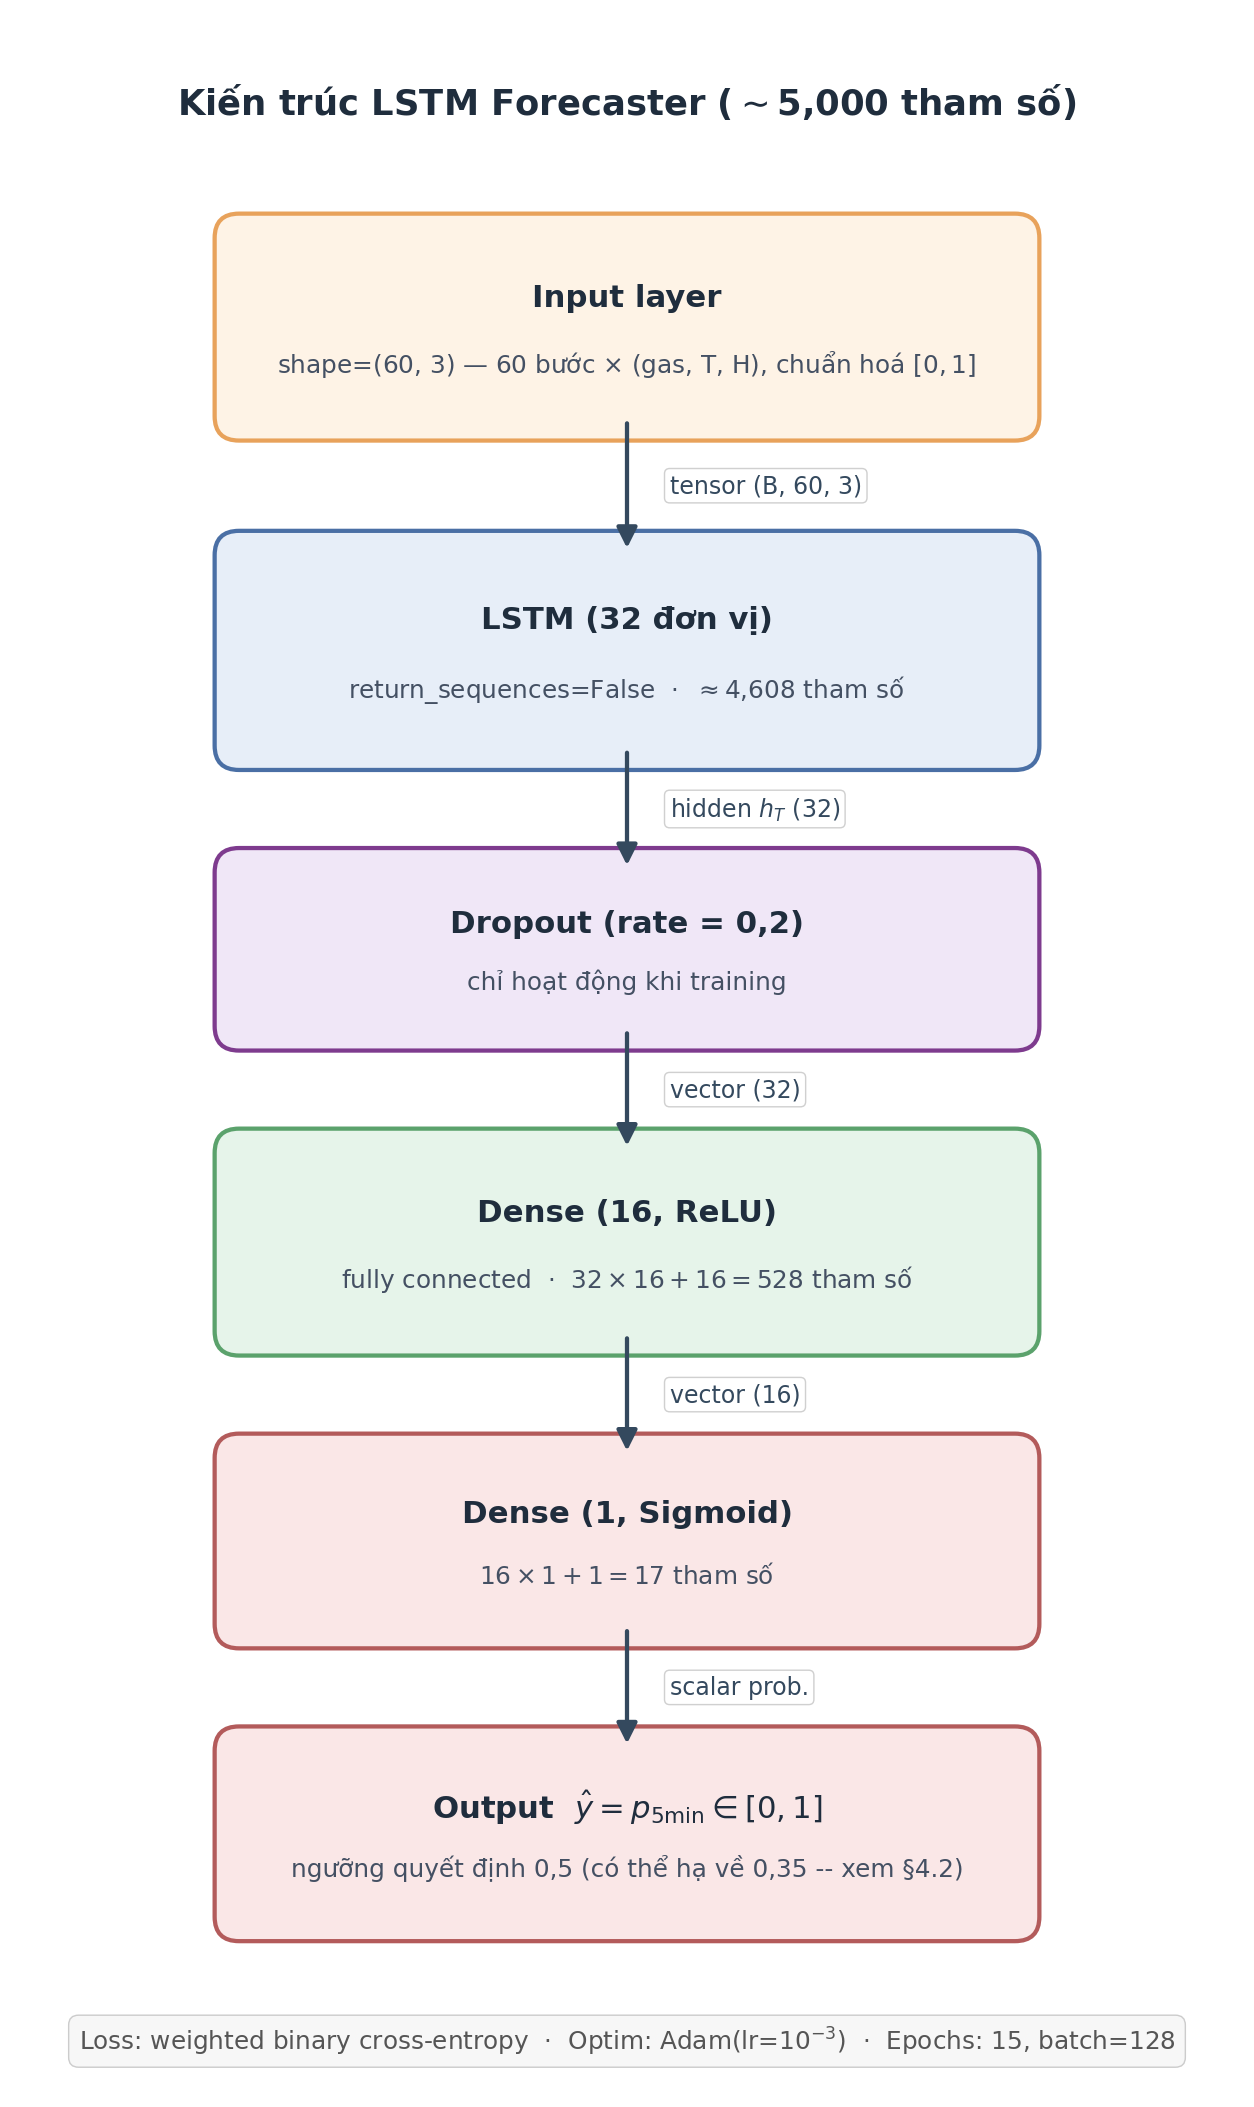
\includegraphics[width=0.62\linewidth]{lstm_arch.png}
  \captionof{figure}{Sơ đồ khối kiến trúc LSTM.}
  \label{fig:lstm_arch}
\end{center}

Trong các hệ thống xử lý dữ liệu theo luồng, mô hình LSTM cần có kích thước phù hợp để giảm thời gian suy luận và đáp ứng yêu cầu xử lý gần thời gian thực. Các thông số cụ thể như số bước thời gian đầu vào, số đặc trưng, ngưỡng dự báo và kiến trúc chi tiết của mô hình sẽ phụ thuộc vào bài toán triển khai cụ thể.

\section{Học tăng cường và thuật toán PPO}

Học tăng cường (Reinforcement Learning -- RL) là một hướng học máy trong đó một tác nhân học cách ra quyết định thông qua quá trình tương tác với môi trường. Tại mỗi bước, tác nhân quan sát trạng thái hiện tại, lựa chọn hành động, nhận phần thưởng và chuyển sang trạng thái mới. Qua nhiều lần tương tác, tác nhân học được chính sách hành động nhằm tối đa hóa tổng phần thưởng tích lũy.

\begin{center}
  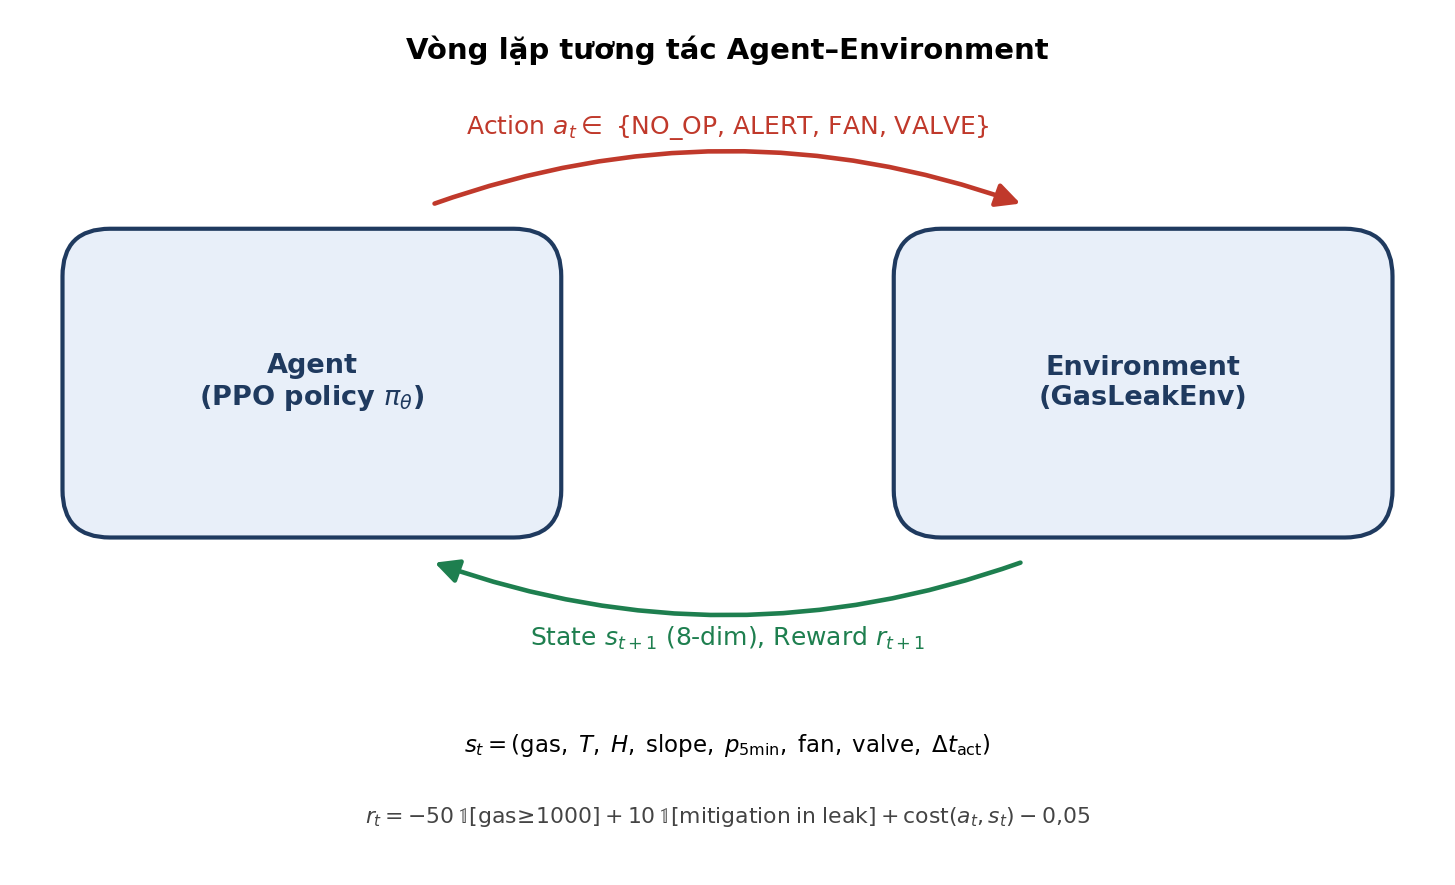
\includegraphics[width=0.65\textwidth]{rl_loop.png}
  \captionof{figure}{Vòng lặp tương tác giữa tác nhân và môi trường trong học tăng cường.}
  \label{fig:rl_loop}
\end{center}

Học tăng cường phù hợp với các bài toán ra quyết định tuần tự, trong đó hành động hiện tại có thể ảnh hưởng đến trạng thái tương lai. So với các luật điều khiển cố định, RL cho phép tác nhân học chính sách hành động thông qua dữ liệu tương tác và hàm thưởng được thiết kế theo mục tiêu của hệ thống.

\subsection{Mô hình MDP}

Bài toán RL thường được mô tả bằng Markov Decision Process (MDP), gồm năm thành phần $(\mathcal{S}, \mathcal{A}, \mathcal{P}, \mathcal{R}, \gamma)$:

\begin{itemize}
  \item $\mathcal{S}$: không gian trạng thái.
  \item $\mathcal{A}$: không gian hành động.
  \item $\mathcal{P}$: xác suất chuyển trạng thái.
  \item $\mathcal{R}$: hàm reward.
  \item $\gamma$: hệ số chiết khấu cho reward tương lai.
\end{itemize}

Trong một bài toán điều khiển, trạng thái có thể bao gồm các biến mô tả môi trường và trạng thái thiết bị; hành động có thể là các lựa chọn điều khiển rời rạc hoặc liên tục. Hàm reward được thiết kế để phản ánh mục tiêu mong muốn, chẳng hạn tăng độ an toàn, giảm chi phí hoặc hạn chế hành động không cần thiết.

\subsection{Proximal Policy Optimization}

Proximal Policy Optimization (PPO) là thuật toán policy gradient được sử dụng rộng rãi nhờ tính ổn định và khả năng triển khai thuận tiện \cite{schulman2017}. PPO cập nhật chính sách theo hướng cải thiện reward, đồng thời giới hạn mức thay đổi của chính sách sau mỗi lần cập nhật. Cơ chế này giúp quá trình học ổn định hơn so với việc cập nhật chính sách quá mạnh.

PPO thường được sử dụng trong các môi trường mô phỏng để huấn luyện tác nhân trước khi đánh giá hoặc triển khai trong hệ thống thực tế. Trong các bài toán có không gian hành động rời rạc, PPO có thể học cách chọn hành động phù hợp dựa trên trạng thái quan sát và tín hiệu phần thưởng từ môi trường.

\section{Docker và container hóa}

\techlogo{docker.jpg}{3cm}{Logo Docker}{fig:Docker_logo}

Docker là nền tảng container hóa cho phép đóng gói ứng dụng cùng thư viện, biến môi trường và cấu hình cần thiết vào các container độc lập. Mỗi container thường chạy một dịch vụ riêng, giúp giảm sự phụ thuộc vào môi trường cài đặt trên máy chủ.

Docker Compose là công cụ dùng để khai báo và quản lý nhiều Docker container thông qua một file cấu hình. Với các hệ thống gồm nhiều dịch vụ, Docker Compose giúp khởi động, dừng, cấu hình mạng và quản lý các container thuận tiện hơn.

Trong phạm vi triển khai thực nghiệm, hệ thống sử dụng Docker Compose để vận hành nhiều container. Docker Compose sẽ là công cụ điều phối các container trong cùng một môi trường chạy.

\section{Cơ sở dữ liệu và hiển thị dữ liệu}

\subsection{InfluxDB và PostgreSQL}

InfluxDB là cơ sở dữ liệu chuỗi thời gian, phù hợp với dữ liệu cảm biến được ghi liên tục theo timestamp. InfluxDB thường được dùng để lưu các bản ghi như nồng độ khí, nhiệt độ, độ ẩm, xác suất dự báo và hành động điều khiển.

\techlogo{influxdb.png}{3cm}{Logo InfluxDB}{fig:influxdb_logo}

PostgreSQL được dùng cho dữ liệu nghiệp vụ có cấu trúc rõ ràng hơn, chẳng hạn lịch sử cảnh báo và lịch sử hành động. Việc tách InfluxDB và PostgreSQL giúp mỗi loại dữ liệu được lưu ở công cụ phù hợp với cách truy vấn của nó: InfluxDB cho chuỗi thời gian, PostgreSQL cho dữ liệu quan hệ.

\techlogo{Postgresql.png}{3cm}{Logo Postgresql}{fig:postgresql_logo}

\subsection{Grafana, bảng điều khiển web và Telegram}

Grafana được dùng để trực quan hóa dữ liệu chuỗi thời gian và hỗ trợ quan sát trạng thái hệ thống trong quá trình thực nghiệm. Bảng điều khiển web có thể hiển thị dữ liệu hiện tại, đồ thị nồng độ khí, xác suất rủi ro và hành động của bộ điều khiển PPO.

\techlogo{grafana.jpg}{3cm}{Logo Grafana}{fig:grafana_logo}

Telegram Bot API được sử dụng như kênh cảnh báo cho người dùng. Khi hệ thống phát hiện nguy cơ hoặc bộ điều khiển chọn hành động cảnh báo, dịch vụ API có thể gửi thông báo đến Telegram kèm thông tin nồng độ khí, mức rủi ro và hành động hiện tại.

\techlogo{Telegram.png}{3cm}{Logo Telegram}{fig:Tele_logo}

\vspace{0.5em}

Tóm lại, chương này đã trình bày các nền tảng chính gồm IoT, giao thức truyền thông, xử lý luồng dữ liệu, LSTM, học tăng cường và PPO, cùng các công cụ lưu trữ/hiển thị dữ liệu. Các khái niệm này là cơ sở để chương tiếp theo mô tả cách hiện thực kiến trúc hệ thống và quy trình huấn luyện, đánh giá.


\chapter{Phương pháp thực hiện}
\label{c:phuongphapthuchien}
% ============================================================
%  Chương 3: Phương pháp thực hiện
% ============================================================

Chương này trình bày cách hiện thực hệ thống từ các nền tảng lý thuyết đã nêu ở Chương~\ref{c:cosolythuyet}. Nội dung chương đi theo luồng từ kiến trúc tổng thể, lớp thiết bị, lớp truyền thông, lớp xử lý, đến lớp ứng dụng và triển khai bằng Docker Compose. Trọng tâm của chương sẽ làm rõ cách mô hình LSTM được xây dựng như một bộ dự báo theo chuỗi thời gian và cách thuật toán PPO được dùng làm bộ điều khiển hành động.

\section{Tổng quan kiến trúc hệ thống}

Hệ thống được thiết kế theo kiến trúc 4 lớp phân tầng rõ ràng, giúp tách biệt vai trò giữa các thành phần và hỗ trợ mở rộng độc lập:

\begin{enumerate}
  \item Lớp thiết bị: ESP32 hoặc bộ mô phỏng phần mềm thu thập và gửi dữ liệu cảm biến.
  \item Lớp truyền thông: Mosquitto MQTT broker và dịch vụ cầu nối MQTT-Kafka.
  \item Lớp xử lý: Apache Spark Structured Streaming tích hợp bộ dự báo LSTM và bộ điều khiển PPO.
  \item Lớp ứng dụng: API Node.js, bảng điều khiển web, Grafana và Telegram bot.
\end{enumerate}

Sơ đồ tổng thể kiến trúc 4 tầng kèm luồng dữ liệu giữa các thành phần được thể hiện trong Hình~\ref{fig:architecture}.

\begin{center}
  \makebox[\textwidth][c]{%
    \hspace*{-1.7cm}%
    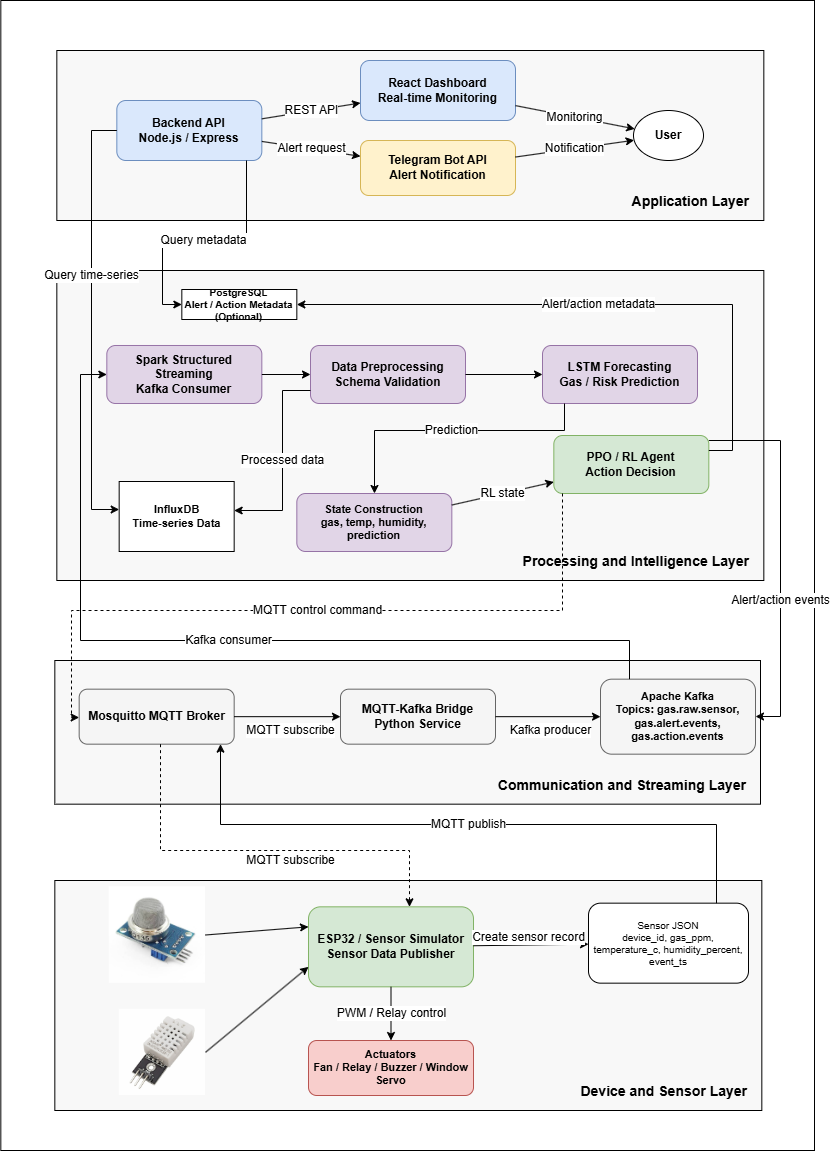
\includegraphics[
      width=1.95\textwidth,
      height=0.95\textheight,
      keepaspectratio
    ]{img/system design.png}%
  }

  \captionof{figure}{Kiến trúc hệ thống 4 tầng.}
  \label{fig:architecture}
\end{center}

\section{Lớp thiết bị}

\subsection{Chương trình ESP32}

Firmware ESP32 được viết bằng ngôn ngữ C++ sử dụng Arduino framework với thư viện PubSubClient cho MQTT. ESP32 đọc dữ liệu từ:
\begin{itemize}
  \item Cảm biến MQ (qua cổng ADC): nồng độ khí gas (ppm)
  \item Cảm biến DHT22: nhiệt độ (°C) và độ ẩm (\%)
\end{itemize}

Mỗi giây (1 Hz), chương trình ESP32 đóng gói dữ liệu thành JSON và gửi lên topic \texttt{sensors/gas}:

\Needspace{12\baselineskip}
\begin{lstlisting}[language=Python, caption={Cấu trúc payload JSON từ thiết bị}]
{
  "device_id": "esp32-lab-01",
  "gas_ppm": 125.43,
  "temperature_c": 28.12,
  "humidity_percent": 61.5,
  "event_ts": 1703123456789
}
\end{lstlisting}

\subsection{Bộ mô phỏng cảm biến}

Do điều kiện thực nghiệm, bộ mô phỏng phần mềm được xây dựng để thay thế phần cứng trong quá trình huấn luyện mô hình và đánh giá so sánh. Bộ mô phỏng triển khai một máy trạng thái vật lý với 4 trạng thái:

\begin{itemize}
  \item NORMAL: Nồng độ nền 50–150 ppm, dao động Gaussian nhỏ. Hàm cập nhật:
  \[gas_t = gas_{t-1} + 0.1(60 - gas_{t-1}) \cdot dt + \mathcal{N}(0, 3) \cdot dt\]

  \item LEAK\_SLOW: Rò rỉ chậm, tốc độ tăng tuyến tính $\sim$5 ppm/s:
  \[gas_t = gas_{t-1} + 5 \cdot dt + \mathcal{N}(0, 2) \cdot dt\]

  \item LEAK\_FAST: Rò rỉ nhanh (vỡ ống), tăng theo hàm mũ:
  \[gas_t = gas_{t-1} \cdot e^{0.04 \cdot dt} + 8 \cdot dt + \mathcal{N}(0, 3) \cdot dt\]

  \item VENTILATING: Sau khi có hành động can thiệp, khí giảm theo hàm mũ:
  \[gas_t = \max(60, gas_{t-1} \cdot e^{-0.03 \cdot dt} - 0.5 \cdot dt)\]
\end{itemize}

Xác suất chuyển trạng thái ngẫu nhiên được tham số hóa qua biến môi trường \texttt{SIM\_LEAK\_PROB\_PER\_MIN} (mặc định 5\% mỗi phút). Trong pha NORMAL, 70\% trường hợp chuyển sang LEAK\_SLOW và 30\% chuyển sang LEAK\_FAST.

Bộ mô phỏng cũng gửi kèm hai trường nhãn thực tế:
\begin{itemize}
  \item \texttt{\_leak\_state}: Trạng thái thực tế (chỉ dùng cho đánh giá).
  \item \texttt{\_seconds\_to\_critical}: Số giây đến khi nồng độ đạt 1000 ppm (ước tính).
\end{itemize}

\section{Lớp truyền thông}

\subsection{Mosquitto MQTT Broker}

Mosquitto là MQTT broker mã nguồn mở nhẹ của Eclipse Foundation. Trong hệ thống, Mosquitto được cấu hình:
\begin{itemize}
  \item Cổng 1883 cho kết nối không mã hóa trong mạng Docker nội bộ.
  \item Bật lưu trạng thái để không mất bản tin khi broker khởi động lại.
  \item Không giới hạn số kết nối trong môi trường phát triển.
\end{itemize}

\subsection{MQTT-Kafka Bridge}

Dịch vụ cầu nối (\texttt{mqtt\_kafka\_bridge.py}) đóng vai trò chuyển bản tin giữa hai giao thức:

\Needspace{12\baselineskip}
\begin{lstlisting}[language=Python, caption={Logic bridge đơn giản hóa}]
def on_message(client, userdata, msg):
    payload = json.loads(msg.payload)
    # Validate and add metadata
    payload['ingested_at'] = int(time.time() * 1000)
    # Chuyen tiep sang Kafka
    producer.produce(
        topic='gas.raw.sensor',
        key=payload['device_id'],
        value=json.dumps(payload),
        callback=delivery_report
    )
    producer.poll(0)
\end{lstlisting}

Dịch vụ cầu nối đăng ký nhận dữ liệu từ MQTT topic \texttt{sensors/gas} và chuyển tiếp lên Kafka topic \texttt{gas.raw.sensor}. Trường \texttt{device\_id} được dùng làm khóa để giữ đúng thứ tự bản tin của từng thiết bị trong Kafka partition.

\section{Lớp xử lý}

\subsection{Luồng xử lý Spark Structured Streaming}

File \texttt{stream\_processor.py} là điểm vào của lớp xử lý. Luồng Spark được thiết kế theo các bước:

Bước 1 – Đọc từ Kafka:
\Needspace{12\baselineskip}
\begin{lstlisting}[language=Python, caption={Đọc luồng dữ liệu từ Kafka}]
raw_stream = (
    spark.readStream
    .format("kafka")
    .option("kafka.bootstrap.servers", KAFKA_BROKERS)
    .option("subscribe", "gas.raw.sensor")
    .option("startingOffsets", "latest")
    .load()
)
\end{lstlisting}

Bước 2 – Phân tích JSON và trích xuất đặc trưng:

Mỗi bản ghi được phân tích từ JSON. Để đưa dữ liệu vào LSTM (cần chuỗi 60 giây), luồng xử lý duy trì một cửa sổ trượt cho từng \texttt{device\_id} trong bộ nhớ. Python UDF nhận chuỗi hiện tại và gọi bộ dự báo:

\Needspace{10\baselineskip}
\begin{lstlisting}[language=Python, caption={Gọi bộ dự báo LSTM trong Spark}]
@udf(returnType=FloatType())
def predict_risk(gas, temp, hum):
    return forecaster.predict(device_id, gas, temp, hum)
\end{lstlisting}

Bước 3 – Gọi bộ điều khiển PPO:

Sau khi có xác suất rủi ro từ LSTM, Spark gọi tác nhân PPO để chọn hành động:

\begin{lstlisting}[language=Python, caption={Gọi tác nhân PPO}]
action, action_name = rl_agent.choose(
    device_id, gas, temp, hum, predicted_risk
)
\end{lstlisting}

Bước 4 – Ghi kết quả:
\begin{itemize}
  \item Ghi vào InfluxDB measurement \texttt{gas\_readings} mọi bản ghi kèm xác suất rủi ro và hành động.
  \item Nếu action $\neq$ NO\_OP, gửi sự kiện lên Kafka topic \texttt{gas.alert.events}.
\end{itemize}

\subsection{Bộ dự báo LSTM}

\subsubsection*{Kiến trúc mô hình}

Mô hình LSTM dự báo được xây dựng bằng Keras/TensorFlow với kiến trúc nhỏ gọn phù hợp với suy luận thời gian thực:

\begin{lstlisting}[
language=Python,
caption={Định nghĩa kiến trúc LSTM},
breaklines=true,
breakatwhitespace=true,
postbreak=\mbox{\textcolor{red}{$\hookrightarrow$}\space}
]
inp = tf.keras.layers.Input(shape=(60, 3))
x = tf.keras.layers.LSTM(32, return_sequences=False)(inp)
x = tf.keras.layers.Dropout(0.2)(x)
x = tf.keras.layers.Dense(16, activation="relu")(x)
out = tf.keras.layers.Dense(1, activation="sigmoid")(x)
model = tf.keras.Model(inp, out)
model.compile(
    optimizer=Adam(1e-3),
    loss="binary_crossentropy",
    metrics=["accuracy", Precision(), Recall()]
)
\end{lstlisting}

Hàm mất mát \texttt{binary\_crossentropy} được dùng vì nhãn huấn luyện là nhãn \emph{dự báo sự kiện}: cửa sổ hiện tại có dẫn đến trạng thái vượt ngưỡng trong 5 phút tới hay không. Đây không phải là bài toán gán nhãn trạng thái tức thời. Nếu mục tiêu được đổi thành dự báo trực tiếp giá trị \texttt{gas\_ppm} tại các thời điểm tương lai, khi đó cần dùng các hàm mất mát và tiêu chí hồi quy như MAE hoặc RMSE.

Tổng số tham số: $\sim$5,000 -- đủ nhỏ để suy luận trong vài millisecond. Sơ đồ khối các lớp được mô tả ở Hình~\ref{fig:lstm_arch} (Chương~\ref{c:cosolythuyet}).

\subsubsection*{Quy trình huấn luyện}

Sinh dữ liệu: Chạy bộ mô phỏng trong $N$ giờ (mặc định 4 giờ) với seed cố định để tạo trace xác định. Trace có dạng mảng $(T, 4)$: $(gas, temp, hum, state\_int)$.

Xây dựng dataset: Với mỗi vị trí $i$ trong trace:
\begin{itemize}
  \item $X[i]$ = chuỗi 60 giây chuẩn hóa kết thúc tại $t$: $feats[i:i+60] / [2000, 60, 100]$
  \item $y[i] = 1$ nếu $\max(gas[i+61:i+361]) > 1000$ else $0$
\end{itemize}

Phân chia train/test: Phân chia theo thứ tự thời gian (80/20), không xáo trộn để tránh data leakage.

Xử lý mất cân bằng: Áp dụng class weight với hệ số:
\[w_{pos} = \frac{1 - p_{pos}}{p_{pos}}, \quad w_{neg} = 1.0\]

trong đó $p_{pos}$ là tỷ lệ mẫu positive trong tập huấn luyện.

\subsubsection*{Hai phiên bản mô hình LSTM được huấn luyện}
\label{sssec:lstm_two_models}

Một điểm cần làm rõ ở mức triển khai là trong đề tài, \emph{cùng một kiến trúc} LSTM (Hình~\ref{fig:lstm_arch}) được huấn luyện thành hai mô hình riêng biệt. Cả hai mô hình đều được đóng gói trong thư mục \texttt{processing/ml/lstm/}, nhưng phục vụ hai mục tiêu đánh giá khác nhau:

\begin{enumerate}
  \item Mô hình mô phỏng (\texttt{gas\_forecaster.keras}): được huấn luyện trên trace 8 giờ sinh từ bộ mô phỏng với seed cố định. Đây là bộ dự báo \emph{mặc định} được nạp trong luồng Spark, do nhãn rò rỉ được xác định rõ và phân phối dữ liệu phù hợp với môi trường mô phỏng dùng để đánh giá so sánh các bộ điều khiển.

  \item Mô hình dữ liệu thực (\texttt{gas\_forecaster\_kaggle.keras}): được huấn luyện trên tập dữ liệu cảm biến IoT thực từ Kaggle. Mô hình này không dùng làm bộ dự báo mặc định trong luồng mô phỏng, mà được sử dụng để kiểm chứng sơ bộ khả năng tổng quát hóa của kiến trúc LSTM trên dữ liệu cảm biến thực.
\end{enumerate}

Bảng~\ref{tab:lstm_two_models} đối chiếu cấu hình huấn luyện của hai mô hình. Điểm mấu chốt là kiến trúc mạng, hàm mất mát và cách xây dựng nhãn theo hướng \emph{dự báo sự kiện} được giữ nhất quán giữa hai mô hình; sự khác biệt chủ yếu nằm ở nguồn dữ liệu, ngưỡng sinh nhãn và một số siêu tham số huấn luyện. Nhờ vậy, kết quả trên tập dữ liệu thực Kaggle có thể được xem là bằng chứng bổ trợ cho thấy kiến trúc LSTM đề xuất có khả năng học xu hướng biến thiên của tín hiệu khí trong nhiều nguồn dữ liệu khác nhau, thay vì chỉ phù hợp với riêng dữ liệu sinh ra từ bộ mô phỏng.

\begingroup
\small
\renewcommand{\arraystretch}{1.25}
\setlength{\tabcolsep}{4pt}

\begin{longtable}{
  >{\raggedright\arraybackslash}p{2.8cm}
  >{\raggedright\arraybackslash}p{5.0cm}
  >{\raggedright\arraybackslash}p{5.0cm}
}
\caption{Đối chiếu hai mô hình LSTM cùng kiến trúc}
\label{tab:lstm_two_models} \\
\toprule
\textbf{Hạng mục} 
& \textbf{Mô hình mô phỏng} 
& \textbf{Mô hình dữ liệu thực (Kaggle)} \\
\midrule
\endfirsthead

% Không lặp lại header nếu bảng bị cắt sang trang mới
\endhead

\bottomrule
\endlastfoot

File trọng số   
& \texttt{gas\_forecaster.keras} 
& \texttt{gas\_forecaster\_kaggle.keras} \\

Nguồn dữ liệu   
& Trace mô phỏng 8\,h, tần số 1\,Hz, seed 42 
& Kaggle Env. Sensor, khoảng 405K mẫu, 3 thiết bị \\

Đặc trưng đầu vào 
& Cửa sổ 60 $\times$ (gas, T, H) 
& Cửa sổ 60 $\times$ (lpg, temp, humidity) \\

Ngưỡng dán nhãn 
& Gas tương lai $> 1000$\,ppm 
& LPG tương lai $> \mathrm{LPG}_{p95}$ \\

Kiến trúc mạng  
& \multicolumn{2}{
    >{\raggedright\arraybackslash}p{10.0cm}
  }{
    \emph{Giống nhau}: Input(60,3) $\rightarrow$ LSTM(32) $\rightarrow$ Dropout(0{,}2) $\rightarrow$ Dense(16) $\rightarrow$ Dense(1)
  } \\

Epochs / batch  
& 20 / 128 
& 25 / 256 \\

Vai trò         
& Bộ dự báo vận hành mặc định 
& Kiểm chứng sơ bộ trên dữ liệu thực \\

\end{longtable}
\endgroup

\subsubsection*{Cơ chế fallback}

Khi mô hình Keras chưa được huấn luyện (file \texttt{.keras} chưa tồn tại), bộ dự báo tự động dùng cơ chế dự phòng bằng ngoại suy xu hướng. Cơ chế này ước tính độ dốc tuyến tính trên 30 mẫu gần nhất bằng \texttt{numpy.polyfit}, sau đó thực hiện ngoại suy tới chân trời $H=300$\,giây. Nếu độ dốc vượt 0{,}5 ppm/s, cơ chế dự phòng bổ sung thêm nhánh ngoại suy mũ bằng cách ước lượng hệ số tăng trưởng trung bình trên 15 mẫu cuối. Giá trị dự báo cuối cùng là \texttt{max(linear, exp)} và được ánh xạ sang xác suất qua hàm logistic với biên $200$\,ppm xung quanh ngưỡng nguy hiểm. Cơ chế này đảm bảo hệ thống vẫn cho ra xác suất dự báo hợp lý ngay cả khi mô hình Keras chưa sẵn sàng, đồng thời chống lại các trường hợp tăng phi tuyến (LEAK\_FAST) mà phép ngoại suy tuyến tính sẽ đánh giá thấp.

\subsection{Bộ điều khiển PPO}

\subsubsection*{Môi trường: \texttt{GasLeakEnv}}

Bài toán điều khiển được mô hình hoá thành một quá trình quyết định Markov (MDP) gồm bốn thành phần: môi trường, không gian trạng thái, không gian hành động và hàm phần thưởng. Bốn thành phần này được trình bày lần lượt trong các mục dưới đây.

\texttt{GasLeakEnv} kế thừa từ \texttt{gymnasium.Env} và bao bọc bộ mô phỏng vật lý đã mô tả ở mục lớp thiết bị, biến nó thành một môi trường tương tác chuẩn cho thuật toán PPO: ở mỗi bước, môi trường nhận một hành động, cập nhật động lực vật lý của phòng (nồng độ khí, trạng thái rò rỉ), rồi trả về trạng thái kế tiếp và phần thưởng tương ứng.

\Needspace{0.62\textheight}
\begin{lstlisting}[
language=Python,
caption={Cấu trúc GasLeakEnv (đã được đơn giản hoá)},
basicstyle=\ttfamily\scriptsize,
lineskip=-1pt
]
class GasLeakEnv(gymnasium.Env):
    observation_space = Box(low=0.0, high=1.0, shape=(8,), dtype=np.float32)
    action_space = Discrete(4)  # NO_OP, ALERT, FAN_ON, CLOSE_VALVE

    def step(self, action):
        leaking = self.world.state in (LEAK_SLOW, LEAK_FAST)

        self._apply_action(action, leaking)
        STEP_FN[self.world.state](self.world, dt=1.0)
        self._apply_ventilation()
        _maybe_transition(self.world, dt=1.0)

        reward = self._compute_reward(action, leaking)
        done = self.t >= self.T
        return self._observe(), reward, False, done, {}
\end{lstlisting}

\subsubsection*{Không gian trạng thái}

Không gian trạng thái là một vector quan sát 8 chiều, mỗi thành phần được chuẩn hoá về $[0,1]$ để mạng policy học ổn định (chi tiết ở Bảng~\ref{tab:rl_state}). Ngoài bốn đại lượng cảm biến/dự báo (nồng độ khí, nhiệt độ, độ ẩm và độ dốc \textit{slope} ước tính trên 30 mẫu cuối) cùng đặc trưng ghép tầng $p_{5\min}$ lấy từ LSTM, trạng thái còn chứa hai cờ nội bộ của bộ điều khiển (\texttt{fan\_on}, \texttt{valve\_closed}) và thời gian kể từ hành động cuối $\Delta t_{\mathrm{act}}$. Hai cờ nội bộ cho phép policy biết các can thiệp đã được kích hoạt để tránh lặp lại không cần thiết.

\begingroup
\small
\renewcommand{\arraystretch}{1.25}
\setlength{\tabcolsep}{4pt}

\begin{longtable}{
  >{\centering\arraybackslash}p{0.8cm}
  >{\raggedright\arraybackslash}p{3.2cm}
  >{\raggedright\arraybackslash}p{8.2cm}
}
\caption{Không gian trạng thái: vector quan sát 8 chiều của \texttt{GasLeakEnv}}
\label{tab:rl_state} \\
\toprule
\textbf{\#} 
& \textbf{Thành phần} 
& \textbf{Ý nghĩa đã chuẩn hoá về $[0,1]$} \\
\midrule
\endfirsthead

% Không lặp lại header nếu bảng bị cắt sang trang mới
\endhead

% Không thêm dòng "Còn tiếp ở trang sau"
\endfoot

\bottomrule
\endlastfoot

1 
& \texttt{gas\_norm}      
& Nồng độ khí chia cho 2000. \\

2 
& \texttt{temp\_norm}     
& Nhiệt độ chia cho 60. \\

3 
& \texttt{hum\_norm}      
& Độ ẩm chia cho 100. \\

4 
& \texttt{slope\_norm}    
& Độ dốc của 30 mẫu gần nhất, được ánh xạ từ khoảng $[-10,10]$ sang $[0,1]$. \\

5 
& $p_{5\mathrm{min}}$             
& Xác suất nguy hiểm trong 5 phút tiếp theo, là đầu ra của mô hình LSTM. \\

6 
& \texttt{fan\_on}        
& Cờ trạng thái cho biết quạt đang bật hay tắt, nhận giá trị $\{0,1\}$. \\

7 
& \texttt{valve\_closed}  
& Cờ trạng thái cho biết van gas đang đóng hay mở, nhận giá trị $\{0,1\}$. \\

8 
& $\Delta t_{\mathrm{act}}$ 
& Thời gian tính từ hành động điều khiển cuối cùng, chia cho 300. \\

\end{longtable}
\endgroup

\subsubsection*{Không gian hành động}

Không gian hành động là tập rời rạc gồm 4 hành động (\texttt{Discrete(4)}); mỗi bước thời gian tác nhân chọn đúng một hành động (Bảng~\ref{tab:rl_action}). Bốn hành động có \emph{chi phí} và \emph{tác động vật lý} rất khác nhau: ALERT rẻ và không làm thay đổi quỹ đạo khí; FAN làm khí giảm chậm ($\sim$1,5\%/giây); còn CLOSE\_VALVE chặn hẳn nguồn rò rỉ nhưng đồng thời cắt nguồn cung khí của hộ gia đình nếu kích hoạt sai lúc. Chính sự bất đối xứng về chi phí này là lý do bài toán được mô hình hóa theo học tăng cường và giải bằng PPO thay vì chỉ dùng một ngưỡng cứng.

\begingroup
\small
\renewcommand{\arraystretch}{1.25}
\setlength{\tabcolsep}{4pt}

\begin{longtable}{
  >{\centering\arraybackslash}p{1.0cm}
  >{\raggedright\arraybackslash}p{3.2cm}
  >{\raggedright\arraybackslash}p{8.0cm}
}
\caption{Không gian hành động: 4 hành động rời rạc của \texttt{GasLeakEnv}}
\label{tab:rl_action} \\
\toprule
\textbf{Mã} 
& \textbf{Hành động} 
& \textbf{Tác động vật lý / chi phí} \\
\midrule
\endfirsthead

% Không lặp lại header nếu bảng bị cắt sang trang mới
\endhead

% Không thêm dòng "Còn tiếp ở trang sau"
\endfoot

\bottomrule
\endlastfoot

0 
& \texttt{NO\_OP}       
& Không làm gì, chỉ chịu chi phí theo từng bước thời gian. \\

1 
& \texttt{ALERT\_USER}  
& Gửi cảnh báo đến người dùng; chi phí thấp và không tác động trực tiếp đến môi trường vật lý. \\

2 
& \texttt{FAN\_ON}      
& Bật quạt thông gió, làm giảm nồng độ khí khoảng $1{,}5\%$/giây. \\

3 
& \texttt{CLOSE\_VALVE} 
& Đóng van gas để chặn nguồn rò rỉ. \\

\end{longtable}
\endgroup

\subsubsection*{Hàm phần thưởng}

Hàm reward được thiết kế theo nguyên tắc \textit{asymmetric cost} kết hợp \textit{outcome-based}: hậu quả của việc bỏ sót rò rỉ (gas vượt ngưỡng nguy hiểm) phải nặng hơn rất nhiều so với cảnh báo sai, và phần thưởng tích cực được trao \emph{theo kết quả} (giữ được khí dưới ngưỡng) thay vì theo hành động:

\begin{align*}
R_t = 
& -0.05 \\
& -50 \cdot \mathbf{1}[gas_t \geq 1000] \\
& +0.3 \cdot \mathbf{1}[leaking \land gas_t < 1000] \\
& + C(action_t, state_t) \\
& + H(state_t).
\end{align*}

\begingroup
\small
\renewcommand{\arraystretch}{1.25}
\setlength{\tabcolsep}{4pt}

\begin{longtable}{
  >{\raggedright\arraybackslash}p{10.2cm}
  >{\centering\arraybackslash}p{2.2cm}
}
\caption{Bộ hệ số reward tham chiếu từ code \texttt{processing/ml/rl/gas\_env.py}}
\label{tab:reward_shape} \\
\toprule
\textbf{Tình huống} 
& \textbf{Reward} \\
\midrule
\endfirsthead

% Không lặp lại header nếu bảng bị cắt sang trang mới
\endhead

% Không thêm dòng "Còn tiếp ở trang sau"
\endfoot

\bottomrule
\endlastfoot

Mỗi bước có $gas \geq 1000$\,ppm, tức hệ thống bỏ sót trạng thái nguy hiểm
& $-50$ \\

Mỗi bước đang rò rỉ nhưng vẫn giữ được $gas < 1000$\,ppm
& $+0{,}3$ \\

Hành động \texttt{ALERT\_USER} khi trạng thái môi trường là \texttt{NORMAL}, tức cảnh báo sai
& $-3$ \\

Hành động \texttt{FAN\_ON} lần đầu khi trạng thái môi trường là \texttt{NORMAL}
& $-15$ \\

Hành động \texttt{CLOSE\_VALVE} lần đầu khi trạng thái môi trường là \texttt{NORMAL}
& $-25$ \\

Giữ van gas ở trạng thái đóng trong môi trường \texttt{NORMAL}, tính theo mỗi bước thời gian
& $-0{,}5$ \\

Giữ quạt thông gió chạy trong môi trường \texttt{NORMAL}, tính theo mỗi bước thời gian
& $-0{,}1$ \\

Chi phí mặc định cho mỗi bước thời gian
& $-0{,}05$ \\

\end{longtable}
\endgroup

Thiết kế hàm thưởng này khắc phục hai vấn đề của phiên bản đầu. \emph{Thứ nhất}, phần thưởng cố định $+10$ cho mỗi lần bấm FAN/VALVE trong lúc rò rỉ bị loại bỏ vì nó cho phép tác nhân tăng điểm thưởng bằng cách lặp lại hành động mà không thực sự kiềm chế được khí, một dạng khai thác sai hàm thưởng. Thay vào đó, phần thưởng $+0{,}3$ chỉ được trao khi khí \emph{thực sự} được giữ dưới ngưỡng trong lúc rò rỉ; vì quạt không thể kiềm chế rò rỉ nhanh (tăng mũ $\sim$4\%/s, trong khi quạt chỉ giảm 1{,}5\%/s), cơ chế này buộc tác nhân học \emph{đóng van} cho LEAK\_FAST. \emph{Thứ hai}, chi phí duy trì ($-0{,}5$ giữ van, $-0{,}1$ giữ quạt trong NORMAL) cùng cơ chế tự khôi phục giúp hạn chế việc chính sách duy trì van hoặc quạt quá lâu khi môi trường đã an toàn: đóng van sai trong NORMAL ngắt nguồn cung khí gas của hộ gia đình, một thiệt hại trải nghiệm thực tế. Hệ số $-50$ cho bước vượt ngưỡng được giữ lớn để ưu tiên tuyệt đối yếu tố an toàn.

\subsubsection*{Huấn luyện PPO}

\Needspace{0.45\textheight}
\begin{lstlisting}[
language=Python,
caption={Cấu hình PPO training},
basicstyle=\ttfamily\scriptsize,
lineskip=-1pt
]
env = make_vec_env(lambda: GasLeakEnv(episode_seconds=1800),
                   n_envs=4, seed=42)
env = VecNormalize(env, norm_obs=False, norm_reward=True, clip_reward=10.0)

model = PPO("MlpPolicy", env,
            n_steps=512, batch_size=128,
            gamma=0.99, gae_lambda=0.95,
            learning_rate=3e-4, ent_coef=0.01)
model.learn(total_timesteps=400_000)
model.save("processing/ml/rl/ppo_gas_agent.zip")
\end{lstlisting}

Bảng~\ref{tab:ppo_hyperparams} tổng hợp các siêu tham số chính của quá trình huấn luyện PPO. Các giá trị này được chọn theo cấu hình ổn định của Stable-Baselines3 cho môi trường hành động rời rạc, đồng thời giữ chi phí huấn luyện phù hợp với phạm vi thực nghiệm.

\begingroup
\small
\renewcommand{\arraystretch}{1.25}
\setlength{\tabcolsep}{4pt}

\begin{longtable}{
  >{\raggedright\arraybackslash}p{3.4cm}
  >{\centering\arraybackslash}p{2.8cm}
  >{\raggedright\arraybackslash}p{6.8cm}
}
\caption{Các siêu tham số chính khi huấn luyện PPO}
\label{tab:ppo_hyperparams} \\
\toprule
\textbf{Siêu tham số} 
& \textbf{Giá trị} 
& \textbf{Ý nghĩa} \\
\midrule
\endfirsthead

% Không lặp lại header nếu bảng bị cắt sang trang mới
\endhead

% Không thêm dòng "Còn tiếp ở trang sau"
\endfoot

\bottomrule
\endlastfoot

Tổng số bước huấn luyện 
& 400{,}000 
& Số bước thời gian tác nhân tương tác với môi trường mô phỏng. \\

Số môi trường song song 
& 4 
& Tăng đa dạng trạng thái quan sát trong quá trình lấy mẫu. \\

Độ dài episode 
& 1{,}800\,s 
& Mỗi episode tương ứng 30 phút mô phỏng. \\

\texttt{n\_steps} 
& 512 
& Số bước thu thập trước mỗi lần cập nhật policy. \\

\texttt{batch\_size} 
& 128 
& Kích thước minibatch khi tối ưu PPO. \\

\texttt{gamma} 
& 0{,}99 
& Hệ số chiết khấu reward tương lai. \\

\texttt{gae\_lambda} 
& 0{,}95 
& Tham số Generalized Advantage Estimation. \\

\texttt{learning\_rate} 
& $3\times10^{-4}$ 
& Tốc độ học của optimizer. \\

\texttt{ent\_coef} 
& 0{,}01 
& Khuyến khích khám phá trong quá trình huấn luyện. \\

\end{longtable}
\endgroup

4 môi trường song song giúp tăng độ đa dạng của dữ liệu huấn luyện và giảm thời gian huấn luyện. Mỗi episode kéo dài 1800 giây (30 phút) mô phỏng. Bộ bọc \texttt{VecNormalize} chuẩn hoá reward giúp đường cong huấn luyện hội tụ rõ ràng và dễ diễn giải (xem Chương~\ref{c:thucnghiemdanhgia}), khắc phục hiện tượng reward kẹt ở vùng âm của phiên bản đầu.

Sơ đồ khối toàn bộ mạng PPO (kiến trúc actor-critic dùng \texttt{MlpPolicy} mặc định của Stable-Baselines3) được thể hiện trong Hình~\ref{fig:ppo_arch}. Phần dùng chung gồm hai lớp Dense 64 đơn vị, kích hoạt $\tanh$; trên đó tách thành hai đầu độc lập: đầu chính sách trả về phân phối xác suất trên 4 hành động qua softmax, đầu giá trị trả về giá trị $V_\phi(s)$ vô hướng. Toàn bộ mạng có khoảng 5{,}000 tham số, nhẹ tương đương bộ dự báo LSTM.

\Needspace{0.55\textheight}
\begin{center}
  \makebox[\textwidth][c]{%
    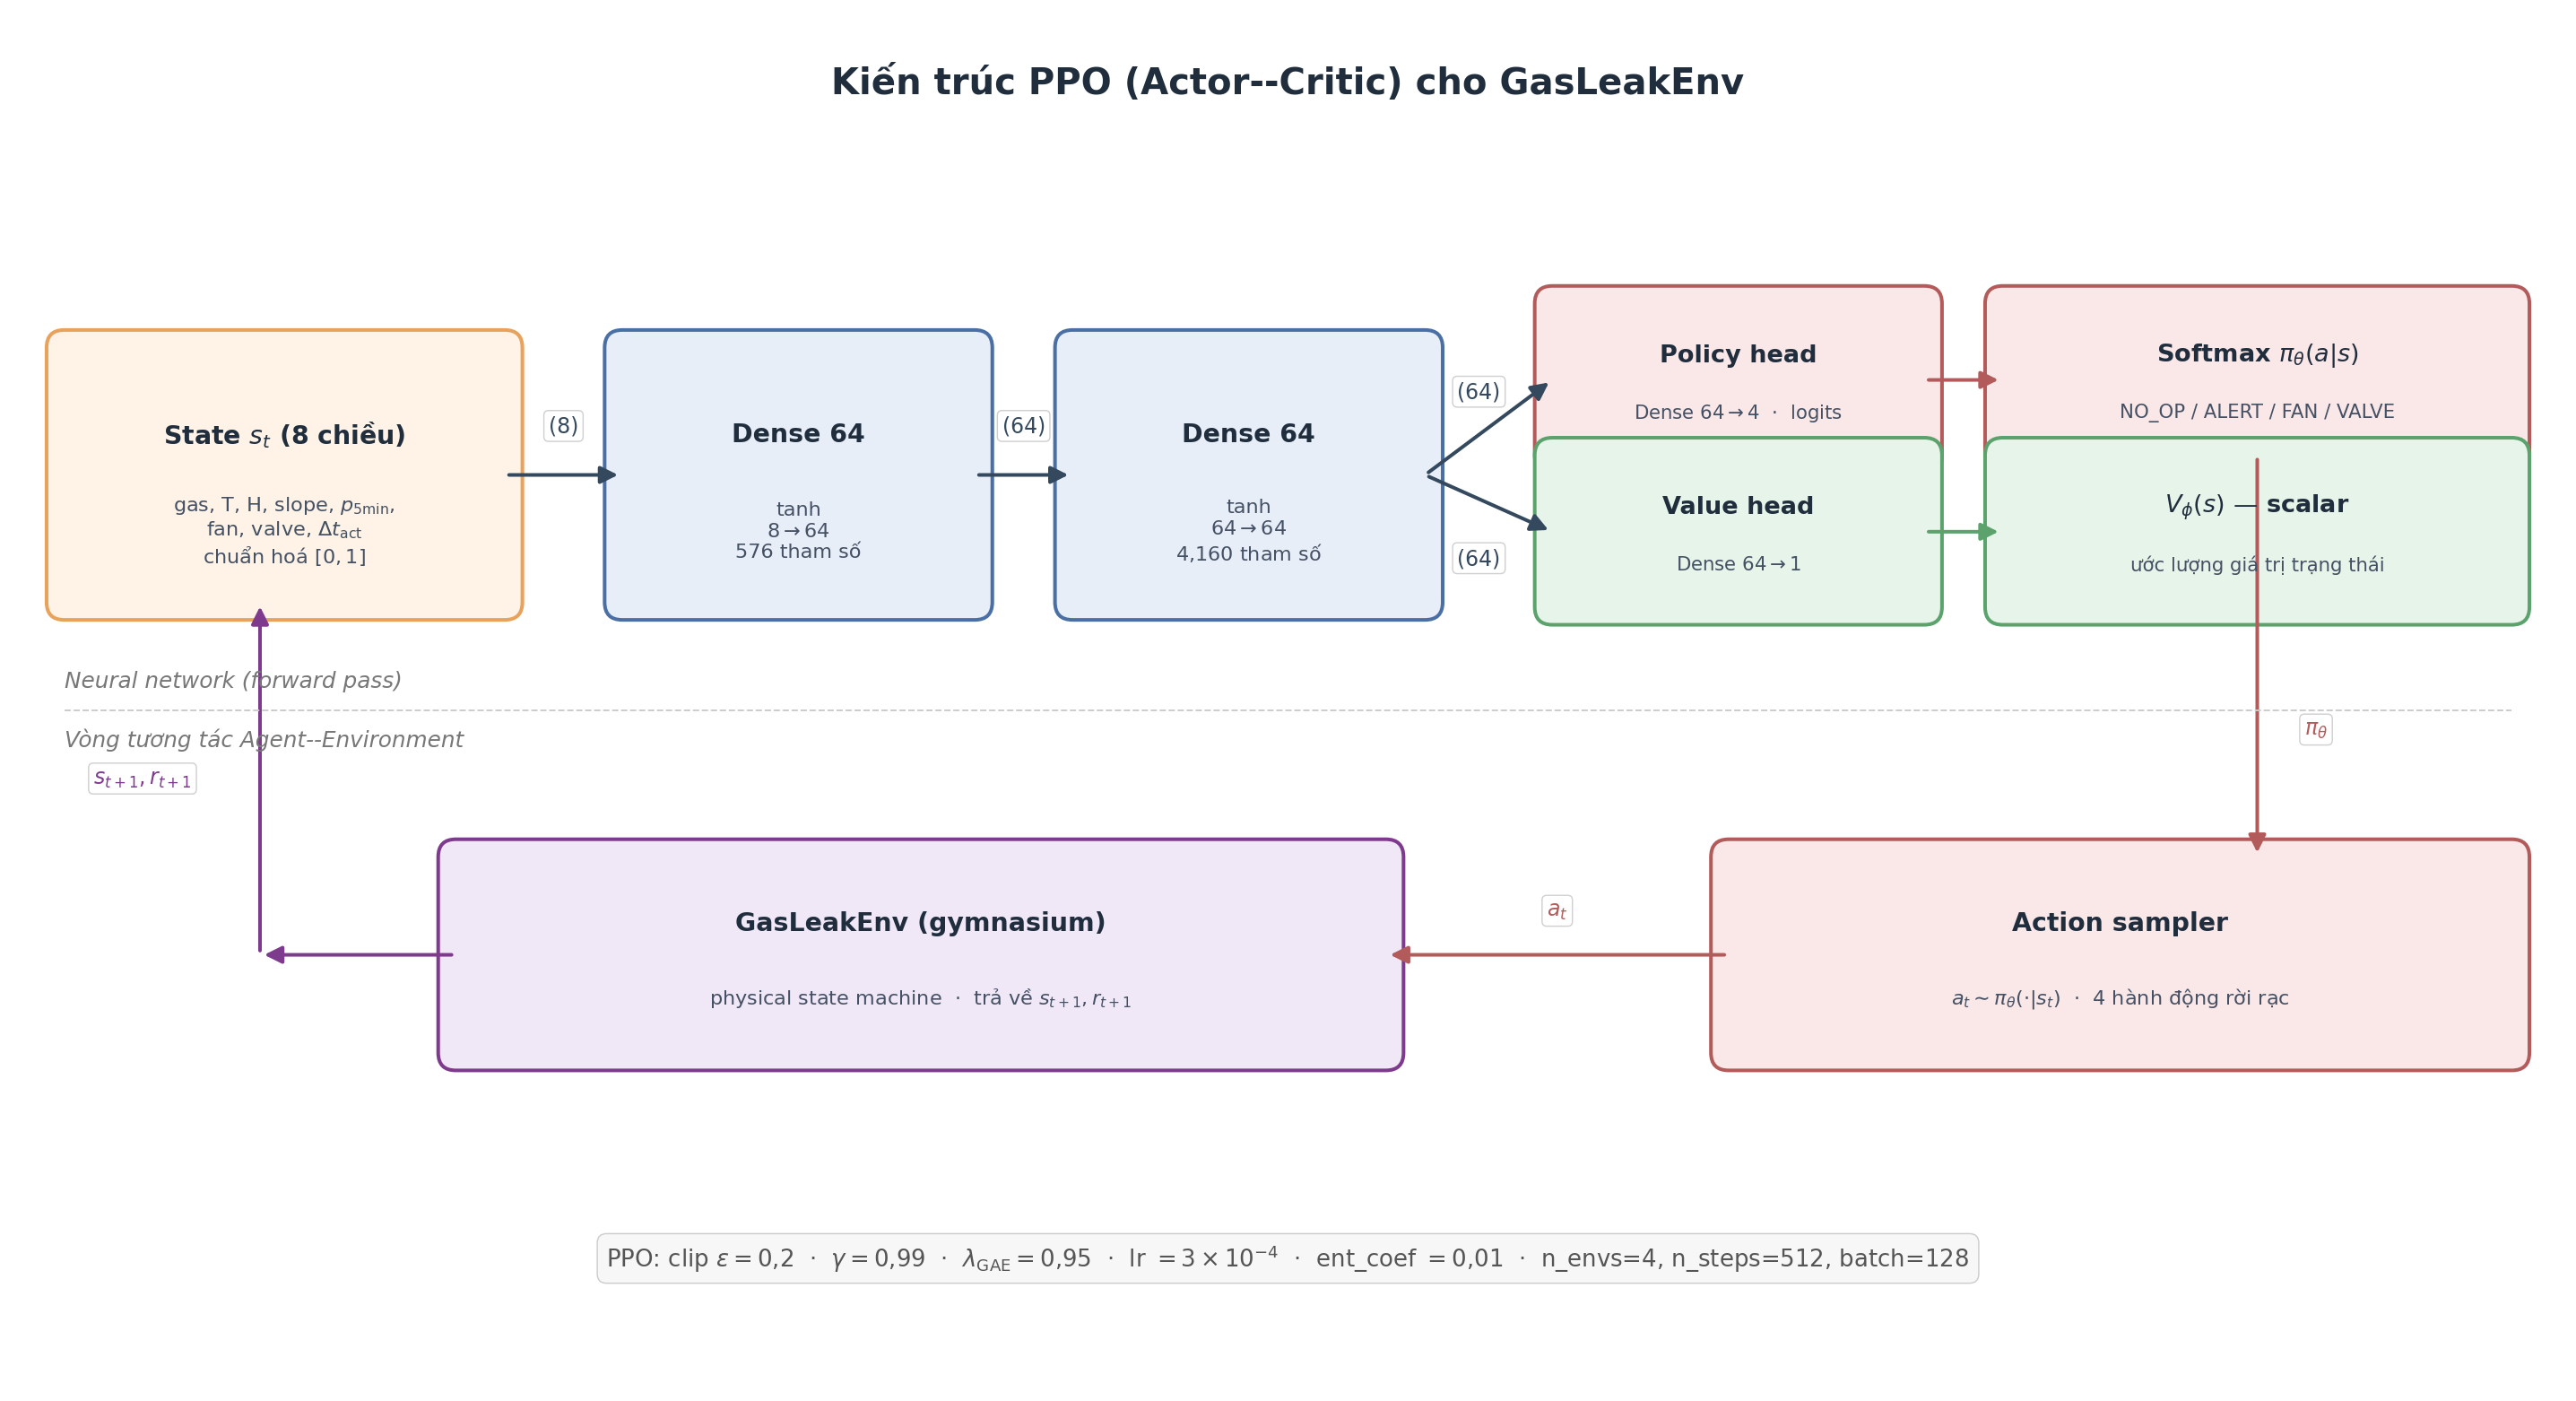
\includegraphics[width=1.18\linewidth]{ppo_arch.png}%
  }
  \captionof{figure}{Sơ đồ khối kiến trúc PPO actor-critic sử dụng Stable-Baselines3 \texttt{MlpPolicy}.}
  \label{fig:ppo_arch}
\end{center}

\subsubsection*{Cơ chế fallback}

Tương tự LSTM, tác nhân PPO có một cơ chế dự phòng theo luật, được kích hoạt khi file PPO chưa tồn tại hoặc tải lỗi. Cơ chế dự phòng bám sát triết lý của hàm thưởng (ưu tiên an toàn, thận trọng với hành động đắt), gồm năm luật được đánh giá theo thứ tự dừng-đầu-tiên:
\begin{enumerate}
  \item Nếu $gas > 800$\,ppm và van chưa đóng $\Rightarrow$ CLOSE\_VALVE.
  \item Nếu $p_{5\min} > 0{,}7$ và van chưa đóng $\Rightarrow$ CLOSE\_VALVE.
  \item Nếu $p_{5\min} > 0{,}4$ hoặc slope $> 1$\,ppm/s, và quạt chưa bật $\Rightarrow$ FAN\_ON.
  \item Nếu $p_{5\min} > 0{,}3$ $\Rightarrow$ ALERT\_USER.
  \item Ngược lại $\Rightarrow$ NO\_OP.
\end{enumerate}
Quy tắc này tham chiếu cả nồng độ tức thời \emph{và} tín hiệu dự báo từ LSTM, đảm bảo hệ thống vẫn có khả năng phản ứng đa cấp ngay cả khi PPO chưa sẵn sàng -- ví dụ ở giai đoạn đầu triển khai hoặc sau khi cập nhật model.

\section{Lớp ứng dụng}

\subsection{API Node.js/TypeScript}

Dịch vụ API được xây dựng bằng Node.js với TypeScript, sử dụng Express.js. Kiến trúc được chia lớp rõ ràng:

\begin{itemize}
  \item Lớp điều phối: xử lý yêu cầu/phản hồi HTTP (\texttt{dashboard.controller.ts}).
  \item Lớp dịch vụ: xử lý nghiệp vụ và kết nối cơ sở dữ liệu (\texttt{influx.service.ts}, \texttt{postgres.service.ts}).
  \item Lớp định tuyến: định nghĩa các điểm truy cập API.
\end{itemize}

Các điểm truy cập REST chính được tóm tắt trong Bảng~\ref{tab:backend_api}.

\begingroup
\small
\renewcommand{\arraystretch}{1.25}
\setlength{\tabcolsep}{4pt}

\begin{longtable}{
  >{\raggedright\arraybackslash}p{4.6cm}
  >{\centering\arraybackslash}p{1.7cm}
  >{\raggedright\arraybackslash}p{6.7cm}
}
\caption{Các điểm truy cập chính của API Node.js}
\label{tab:backend_api} \\
\toprule
\textbf{Điểm truy cập} 
& \textbf{Phương thức} 
& \textbf{Vai trò} \\
\midrule
\endfirsthead

% Không lặp lại header nếu bảng bị cắt sang trang mới
\endhead

% Không thêm dòng "Còn tiếp ở trang sau"
\endfoot

\bottomrule
\endlastfoot

\texttt{/api/dashboard/latest} 
& GET 
& Đọc bản ghi mới nhất từ InfluxDB. \\

\texttt{/api/dashboard/history} 
& GET 
& Đọc lịch sử nồng độ khí trong một khoảng thời gian. \\

\texttt{/api/dashboard/alerts} 
& GET 
& Đọc lịch sử cảnh báo từ PostgreSQL. \\

\texttt{/api/dashboard/actions} 
& GET 
& Đọc lịch sử hành động của bộ điều khiển PPO từ PostgreSQL. \\

\texttt{/api/events} 
& GET/SSE 
& Cung cấp luồng cập nhật thời gian thực cho bảng điều khiển web. \\

\end{longtable}
\endgroup

Dịch vụ API cũng đọc từ Kafka topic \texttt{gas.alert.events} để phát SSE đến trình duyệt và kích hoạt thông báo Telegram.

\subsection{Bảng điều khiển web}

Giao diện web được triển khai như một container riêng, hiển thị giao diện React tại cổng 8080. Thành phần này không xử lý nghiệp vụ trực tiếp mà gọi REST API từ dịch vụ API và nhận luồng cập nhật thời gian thực qua SSE:

\begin{itemize}
  \item Đồng hồ rủi ro: hiển thị xác suất rủi ro 5 phút (0–100\%) cập nhật gần thời gian thực qua SSE.
  \item Biểu đồ chuỗi thời gian: hiển thị nồng độ khí gas theo thời gian thực.
  \item Thẻ hành động PPO: hiển thị hành động hiện tại của bộ điều khiển PPO.
  \item Bảng lịch sử cảnh báo: hiển thị các cảnh báo gần nhất.
\end{itemize}

Mã JavaScript phía trình duyệt kết nối tới điểm SSE của dịch vụ API và cập nhật giao diện mà không cần tải lại trang. Cách tách giao diện web thành container riêng giúp màn hình giám sát có thể phát triển độc lập với API Node.js, đúng với bố trí trong sơ đồ triển khai ở Hình~\ref{fig:system_implementation}.

\subsection{Telegram Bot}

Telegram bot được tích hợp vào dịch vụ API. Khi nhận sự kiện cảnh báo từ tiến trình đọc Kafka:

\Needspace{12\baselineskip}
\begin{lstlisting}[language=Python, caption={Gửi cảnh báo qua Telegram}]
async def send_alert(gas_ppm, risk, action):
    message = (
        f"GAS LEAK ALERT\n"
        f"Concentration: {gas_ppm:.1f} ppm\n"
        f"Five-minute risk: {risk*100:.1f}%\n"
        f"Action: {action}"
    )
    await bot.send_message(chat_id=CHAT_ID, text=message)
\end{lstlisting}

Người dùng cũng có thể tương tác với bot qua các lệnh:
\begin{itemize}
  \item \texttt{/status}: Xem trạng thái hiện tại của hệ thống.
  \item \texttt{/history}: Xem 5 cảnh báo gần nhất.
  \item \texttt{/subscribe}/\texttt{/unsubscribe}: Đăng ký/hủy nhận cảnh báo tự động.
\end{itemize}

\subsection{Bảng điều khiển Grafana}

Grafana kết nối trực tiếp với InfluxDB để hiển thị các biểu đồ phân tích:
\begin{itemize}
  \item Biểu đồ nồng độ khí gas, nhiệt độ, độ ẩm theo thời gian.
  \item Biểu đồ xác suất rủi ro dự báo theo thời gian.
  \item Phân phối hành động PPO (histogram).
  \item Thống kê số cảnh báo theo giờ/ngày.
\end{itemize}

Bảng điều khiển được tạo cấu hình tự động khi khởi động thông qua thư mục \texttt{infrastructure/grafana/provisioning/}.


\section{Triển khai với Docker Compose}

Toàn bộ hệ thống được định nghĩa trong \texttt{docker-compose.yml} với mạng nội bộ \texttt{iot-network}. Thứ tự khởi động được kiểm soát qua \texttt{depends\_on} với \texttt{condition: service\_healthy}:

\begin{enumerate}
  \item Mosquitto, Zookeeper khởi động đầu tiên.
  \item Kafka khởi động sau Zookeeper healthy.
  \item InfluxDB, PostgreSQL khởi động song song.
  \item mqtt-kafka-bridge, device-simulator khởi động sau Mosquitto và Kafka healthy.
  \item processing-engine khởi động sau Kafka, InfluxDB, PostgreSQL healthy.
  \item Dịch vụ API khởi động sau lớp xử lý.
  \item Giao diện web và Grafana khởi động cuối.
\end{enumerate}

Tất cả biến cấu hình (broker URLs, credentials, topic names) được quản lý qua file \texttt{.env}, không hardcode trong code.

\subsection{Sơ đồ triển khai container}
Hình~\ref{fig:system_implementation} mô tả cách các thành phần trên được ánh xạ thành các container và luồng trao đổi dữ liệu trong môi trường Docker Compose. Dữ liệu cảm biến được gửi từ ESP32 hoặc bộ mô phỏng lên Mosquitto qua topic \texttt{sensors/gas}, sau đó dịch vụ MQTT-Kafka Bridge chuyển tiếp sang Kafka để Spark Streaming xử lý. Khối Spark đọc luồng dữ liệu, suy luận LSTM, gọi tác nhân PPO, rồi ghi kết quả dự báo, cảnh báo và hành động xuống InfluxDB/PostgreSQL. Ở lớp ứng dụng, bảng điều khiển React gọi REST API từ dịch vụ Node.js/Express, Grafana đọc trực tiếp InfluxDB, còn dịch vụ API gửi thông báo qua Telegram Bot API khi có sự kiện cảnh báo hoặc hành động. Đường điều khiển ngược về thiết bị được thể hiện bằng topic \texttt{home/control}.

\vspace{0.5em}
\begin{center}
  \hspace*{-0.8cm}%
  \makebox[\textwidth][l]{%
    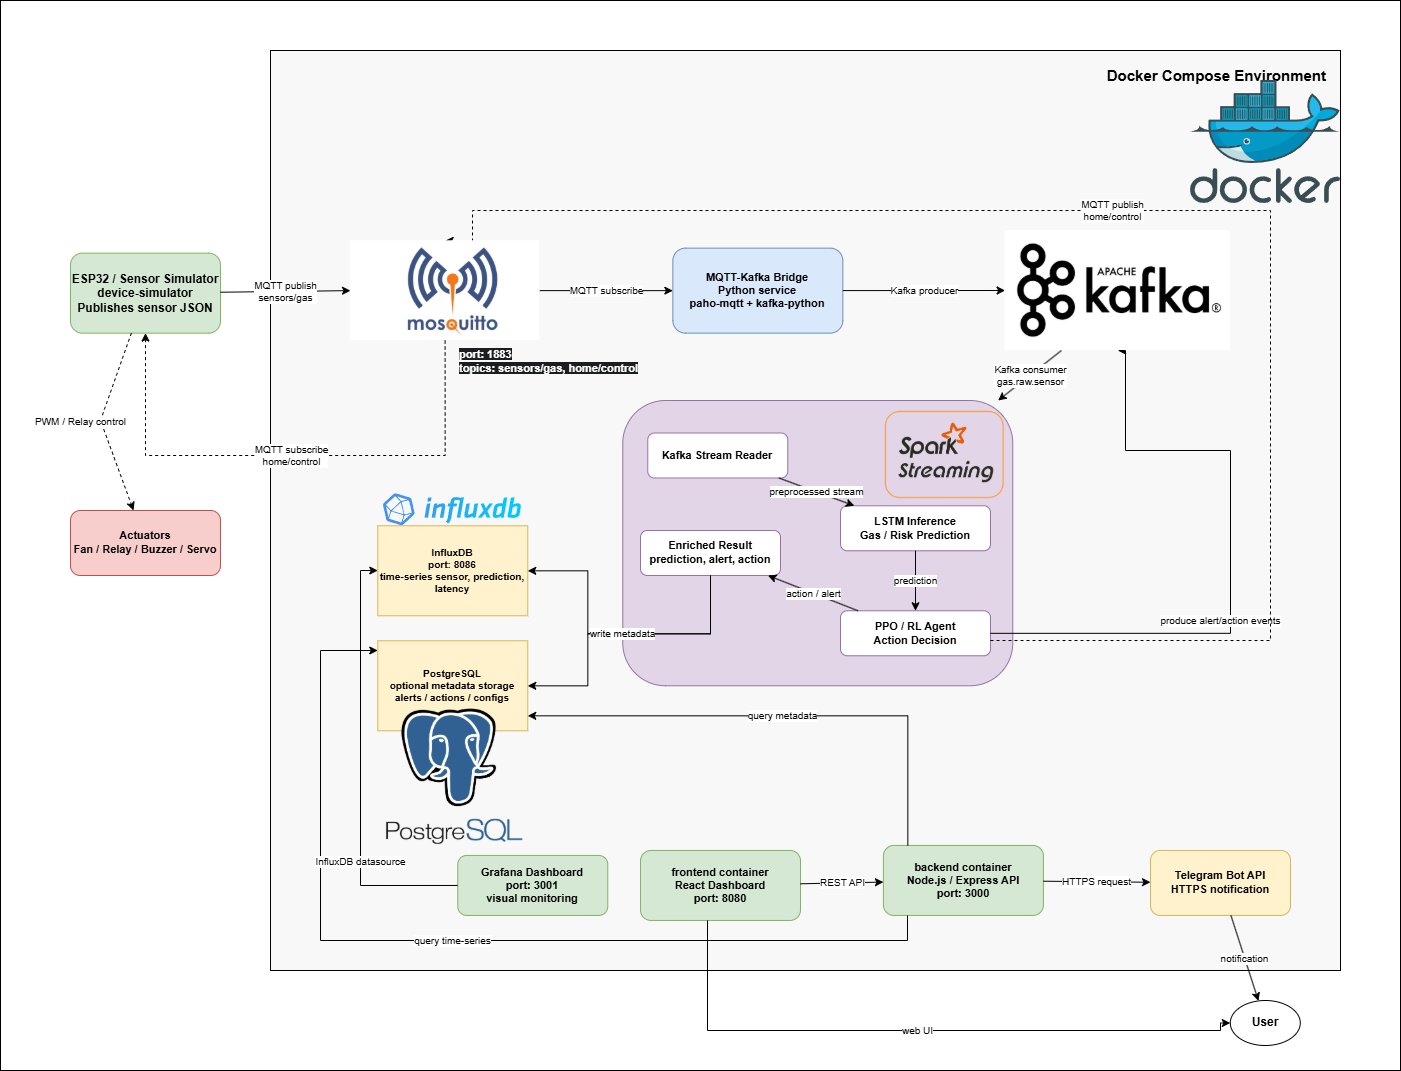
\includegraphics[
      width=1.15\textwidth,
      height=0.8\textheight,
      keepaspectratio
    ]{system implementation.png}%
  }

  \captionof{figure}{Mô hình triển khai hệ thống.}
  \label{fig:system_implementation}
\end{center}

\vspace{0.5em}
Tóm lại, chương này đã mô tả toàn bộ phương pháp hiện thực hệ thống, từ thiết bị, mô phỏng, truyền thông đến xử lý luồng dữ liệu, dự báo LSTM, điều khiển PPO và cuối cùng là lớp ứng dụng. Các cấu hình mô hình, cơ chế dự phòng và triển khai container được trình bày để làm rõ cách hệ thống có thể chạy lại trong môi trường thực nghiệm. Chương tiếp theo sử dụng các thành phần này để đánh giá dữ liệu, mô hình, bộ điều khiển và luồng triển khai.


\chapter{Thực nghiệm, đánh giá và thảo luận}
\label{c:thucnghiemdanhgia}
% ============================================================
%  Chương 4: Thực nghiệm, đánh giá và thảo luận
% ============================================================

Chương này trình bày kết quả thực nghiệm của hệ thống sau khi các thành phần đã được thiết kế và hiện thực ở Chương~\ref{c:phuongphapthuchien}. Nội dung chương được tổ chức theo hai nhóm chính. Nhóm thứ nhất trình bày kết quả huấn luyện và kiểm chứng các mô hình LSTM và PPO. Nhóm thứ hai trình bày các kịch bản đánh giá hệ thống, bao gồm benchmark bộ điều khiển, testcase vận hành LSTM/PPO, kiểm thử pipeline dữ liệu và đo độ trễ suy luận. Các kết quả được diễn giải trong phạm vi mô phỏng và kiểm thử phần mềm, không thay thế cho kiểm định an toàn trên phần cứng gas thực.

\section{Mục tiêu và phạm vi thực nghiệm}
Mục tiêu của phần thực nghiệm là đánh giá toàn bộ hệ thống khi các thành phần IoT, xử lý luồng dữ liệu, dự báo LSTM và điều khiển học tăng cường PPO phối hợp với nhau. Các nội dung đánh giá được tổ chức theo các nội dung sau:

\begin{enumerate}
  \item Đánh giá kết quả huấn luyện mô hình LSTM trong bài toán dự báo rủi ro nồng độ khí gas.
  \item Đánh giá quá trình học và chính sách điều khiển của PPO trong môi trường mô phỏng.
  \item Đánh giá hệ thống qua các kịch bản vận hành, benchmark bộ điều khiển, pipeline dữ liệu và độ trễ xử lý.
\end{enumerate}

Do chưa triển khai kiểm thử an toàn trên phần cứng gas thật, các kết quả trong chương này được hiểu là kết quả kiểm chứng trong môi trường phần mềm có kiểm soát. Dữ liệu công khai được dùng để tham chiếu và kiểm chứng bổ sung cho mô hình LSTM, còn bộ mô phỏng được dùng để tạo nhãn huấn luyện chính, tạo kịch bản vận hành và kiểm thử tích hợp hệ thống.

\section{Môi trường thực nghiệm}

\subsection{Cấu hình phần cứng và phần mềm}

Các thí nghiệm được thực hiện trên máy cá nhân có Docker, đồng thời một số quá trình huấn luyện mô hình được chạy trên Google Colab. Bảng~\ref{tab:env_hardware} mô tả môi trường thực nghiệm chính.

\begingroup
\small
\renewcommand{\arraystretch}{1.25}
\setlength{\LTleft}{0pt}
\setlength{\LTright}{0pt}

\begin{longtable}{
  >{\raggedright\arraybackslash}p{4cm}
  >{\raggedright\arraybackslash}p{\dimexpr\textwidth-4cm-4\tabcolsep\relax}
}
\caption{Cấu hình môi trường thực nghiệm}
\label{tab:env_hardware} \\
\toprule
\textbf{Thành phần} & \textbf{Mô tả} \\
\midrule
\endfirsthead
\toprule
\textbf{Thành phần} & \textbf{Mô tả} \\
\midrule
\endhead
\endfoot
\bottomrule
\endlastfoot

Máy thực nghiệm 
& Laptop/máy trạm cá nhân, Windows 11, Docker Desktop/WSL2 \\

CPU/RAM 
& CPU đa nhân, RAM 16GB \\

Huấn luyện mô hình 
& Môi trường Google Colab CPU và môi trường Python cục bộ \\

Môi trường container 
& Docker Compose \\

Ngôn ngữ 
& Python, TypeScript/JavaScript, PowerShell \\

Message protocol 
& MQTT \\

Message broker 
& Apache Kafka \\

Xử lý luồng dữ liệu 
& Apache Spark Structured Streaming \\

Database 
& InfluxDB cho dữ liệu chuỗi thời gian; PostgreSQL cho lịch sử cảnh báo và hành động \\

Giao diện 
& Bảng điều khiển web, Grafana, Telegram bot \\

\end{longtable}
\endgroup

\section{Dữ liệu thực nghiệm}
\label{sec:dataset_role}
\subsection{Tập dữ liệu kiểm chứng}
\label{ssec:validated_dataset}
Tập dữ liệu công khai đầu tiên được khảo sát là \textit{UCI Gas Sensor Array Under Dynamic Gas Mixtures}. Đây là tập dữ liệu chuỗi thời gian đa biến, được thu từ 16 cảm biến khi tiếp xúc với các hỗn hợp khí thay đổi động theo thời gian. Theo mô tả của UCI Machine Learning Repository, dữ liệu được thu liên tục với tần số 100\,Hz, gồm hai hỗn hợp khí chính: Ethylene--Methane và Ethylene--CO trong không khí~\cite{uci_gas_dynamic}.

UCI được dùng như nguồn tham chiếu về đặc tính chuỗi thời gian của cảm biến khí: tín hiệu có quán tính, nhiễu và thay đổi theo quá trình phơi nhiễm khí. Tuy nhiên, tập này không cùng cấu trúc dữ liệu với luồng triển khai, không chứa LPG dân dụng, nhiệt độ--độ ẩm theo cách hệ thống sử dụng và không có nhãn hành động điều khiển. Vì vậy, UCI không được dùng làm dữ liệu huấn luyện khi hệ thống vận hành, mà được dùng để củng cố cơ sở lựa chọn hướng dự báo chuỗi thời gian.

\begingroup
\footnotesize
\renewcommand{\arraystretch}{1.35}
\setlength{\tabcolsep}{3pt}
\setlength{\LTleft}{0pt}
\setlength{\LTright}{0pt}

\begin{longtable}{
  >{\raggedright\arraybackslash}p{3.0cm}
  >{\centering\arraybackslash}p{2.3cm}
  >{\centering\arraybackslash}p{1.8cm}
  >{\raggedright\arraybackslash}p{\dimexpr\textwidth-7.1cm-8\tabcolsep\relax}
}
\caption{Mô tả các file dữ liệu trong tập UCI Gas Sensor Array Under Dynamic Gas Mixtures}
\label{tab:uci_gas_dataset} \\
\toprule
\textbf{File dữ liệu} 
& \textbf{Số điểm dữ liệu} 
& \textbf{Số thuộc tính} 
& \textbf{Mô tả thuộc tính} \\
\midrule
\endfirsthead
\toprule
\textbf{File dữ liệu} 
& \textbf{Số điểm dữ liệu} 
& \textbf{Số thuộc tính} 
& \textbf{Mô tả thuộc tính} \\
\midrule
\endhead
\endfoot
\bottomrule
\endlastfoot

\makecell[l]{\texttt{ethylene\_}\\\texttt{methane.txt}}
& 4{,}208{,}261
& 19
& Thời gian, nồng độ Methane, nồng độ Ethylene và 16 kênh tín hiệu cảm biến. \\

\makecell[l]{\texttt{ethylene\_}\\\texttt{CO.txt}}
& 4{,}178{,}504
& 19
& Thời gian, nồng độ CO, nồng độ Ethylene và 16 kênh tín hiệu cảm biến. \\

\end{longtable}
\endgroup

Hình~\ref{fig:uci_dataset_histogram} bổ sung góc nhìn trực quan về quy mô hai file dữ liệu trong tập UCI. Hai file có số điểm dữ liệu xấp xỉ nhau, đều trên 4 triệu mẫu, cho thấy đây là tập dữ liệu chuỗi thời gian đủ dài để tham chiếu đặc tính động của cảm biến khí. Tuy nhiên, histogram này chỉ dùng để mô tả quy mô tập kiểm chứng, không hàm ý UCI được dùng trực tiếp làm dữ liệu huấn luyện vận hành.

\Needspace{0.45\textheight}
\begin{center}
  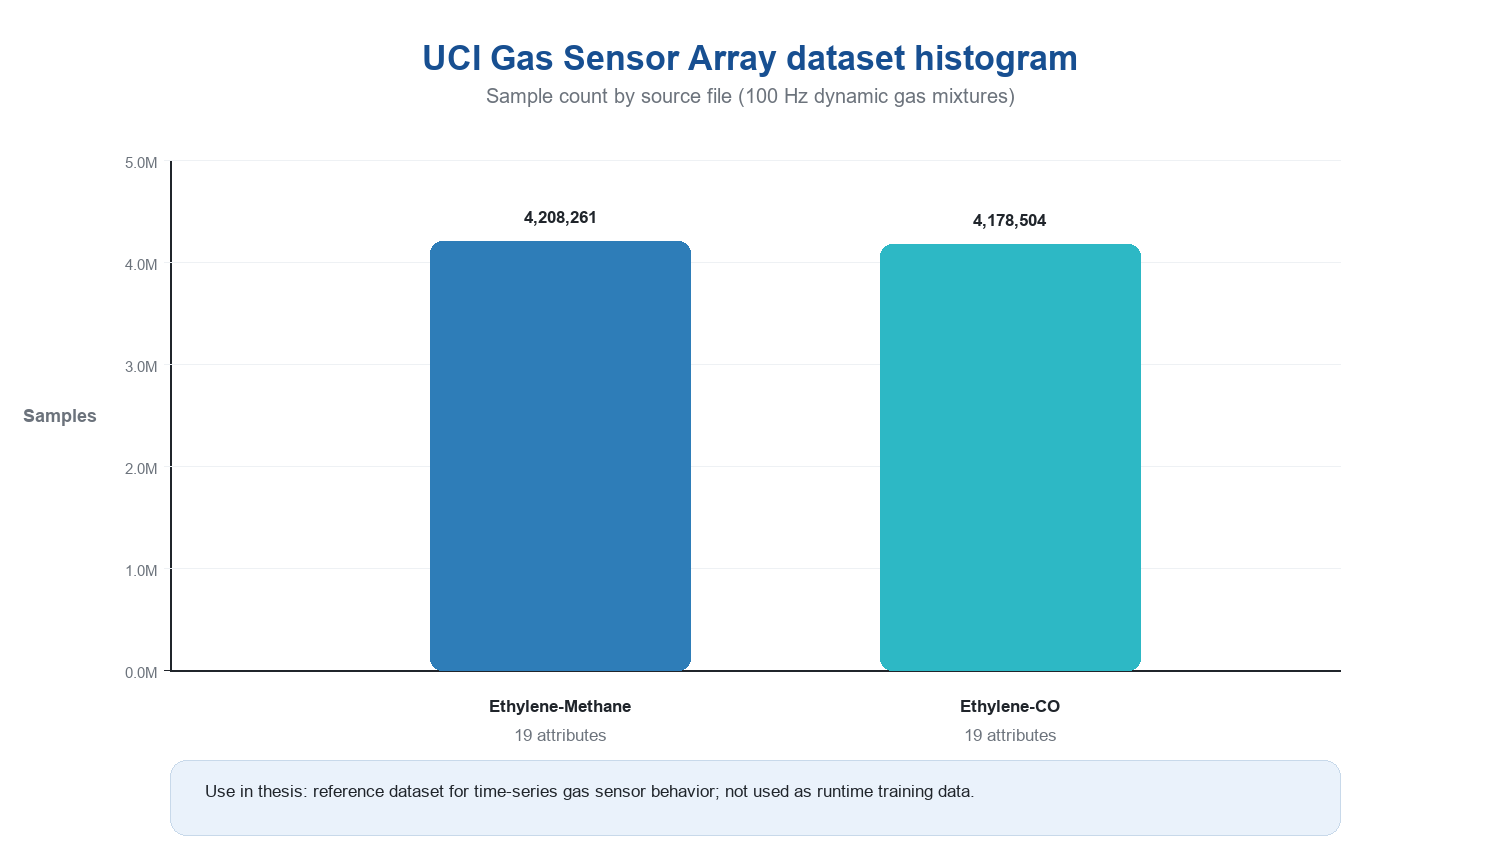
\includegraphics[width=0.92\linewidth]{exp/uci_dataset_histogram.png}
  \captionof{figure}{Histogram quy mô hai file dữ liệu trong tập UCI theo số điểm dữ liệu.}
  \label{fig:uci_dataset_histogram}
\end{center}

Về kết quả huấn luyện trên UCI, khóa luận không trình bày một bảng đánh giá riêng vì mô hình LSTM hiện tại không được huấn luyện trực tiếp trên tập này. UCI chứa Methane/Ethylene/CO và 16 kênh cảm biến, trong khi pipeline của hệ thống dùng \texttt{gas\_ppm}, temperature, humidity và nhãn sự kiện ``vượt ngưỡng trong 5 phút tới''. Nếu ép UCI thành bài toán dự báo nồng độ CO/Methane liên tục thì đó là một thí nghiệm hồi quy khác, cần đánh giá bằng MAE/RMSE/R\textsuperscript{2} theo đơn vị khí tương ứng, không so sánh trực tiếp với đầu ra \texttt{predicted\_risk\_5min}. Vì vậy, UCI chỉ được dùng làm dataset tham chiếu để giải thích đặc tính chuỗi thời gian của cảm biến khí.

Ngoài UCI dataset, đề tài sử dụng thêm tập \textit{Environmental Sensor Telemetry Data} từ Kaggle để kiểm chứng bổ sung trên dữ liệu cảm biến IoT thực~\cite{stafford2020envsensor}. Tập dữ liệu này chứa tín hiệu LPG, CO, smoke, nhiệt độ và độ ẩm từ các thiết bị IoT sử dụng Raspberry Pi, gần với cấu trúc đầu vào của LSTM hơn UCI. Tuy nhiên, dữ liệu không cung cấp nhãn rò rỉ LPG thật, do đó nhãn dương chỉ được xây dựng theo quy tắc proxy dựa trên phân vị cao của tín hiệu LPG. Vì vậy, kết quả trên Kaggle chỉ dùng để kiểm tra sơ bộ khả năng học xu hướng của kiến trúc LSTM trên dữ liệu cảm biến thực, không dùng để kết luận an toàn.

\begingroup
\footnotesize
\renewcommand{\arraystretch}{1.35}
\setlength{\tabcolsep}{4pt}
\setlength{\LTleft}{0pt}
\setlength{\LTright}{0pt}

\begin{longtable}{
  >{\raggedright\arraybackslash}p{3.2cm}
  >{\centering\arraybackslash}p{2.4cm}
  >{\centering\arraybackslash}p{2.0cm}
  >{\raggedright\arraybackslash}p{\dimexpr\textwidth-7.6cm-8\tabcolsep\relax}
}
\caption{Mô tả tập dữ liệu Environmental Sensor Telemetry Data từ Kaggle}
\label{tab:kaggle_env_sensor_dataset} \\
\toprule
\textbf{Tên tập dữ liệu} 
& \textbf{Số điểm dữ liệu} 
& \textbf{Số thuộc tính} 
& \textbf{Mô tả thuộc tính} \\
\midrule
\endfirsthead
\toprule
\textbf{Tên tập dữ liệu} 
& \textbf{Số điểm dữ liệu} 
& \textbf{Số thuộc tính} 
& \textbf{Mô tả thuộc tính} \\
\midrule
\endhead
\endfoot
\bottomrule
\endlastfoot

\makecell[l]{\textit{Environmental}\\\textit{Sensor Telemetry}\\\textit{Data}}
& 405{,}184
& 9
& Timestamp, \texttt{device\_id}, CO, humidity, light, LPG, motion, smoke, temperature. \\

\end{longtable}
\endgroup

Hình~\ref{fig:kaggle_dataset_histogram} mô tả số dòng thô của Kaggle dataset và phân bố các cửa sổ chuỗi thời gian sau khi gán nhãn sự kiện tương lai. Phần màu vàng biểu diễn các cửa sổ dương theo nhãn proxy, tức là cửa sổ hiện tại dẫn đến tín hiệu LPG cao trong chân trời dự báo. Tỷ lệ dương trên tập kiểm thử chỉ khoảng 1{,}31\%, vì vậy khi quan sát tầng cảnh báo sau ngưỡng trên Kaggle cần xem Recall, Precision và ma trận nhầm lẫn thay vì chỉ nhìn Accuracy.

\Needspace{0.45\textheight}
\begin{center}
  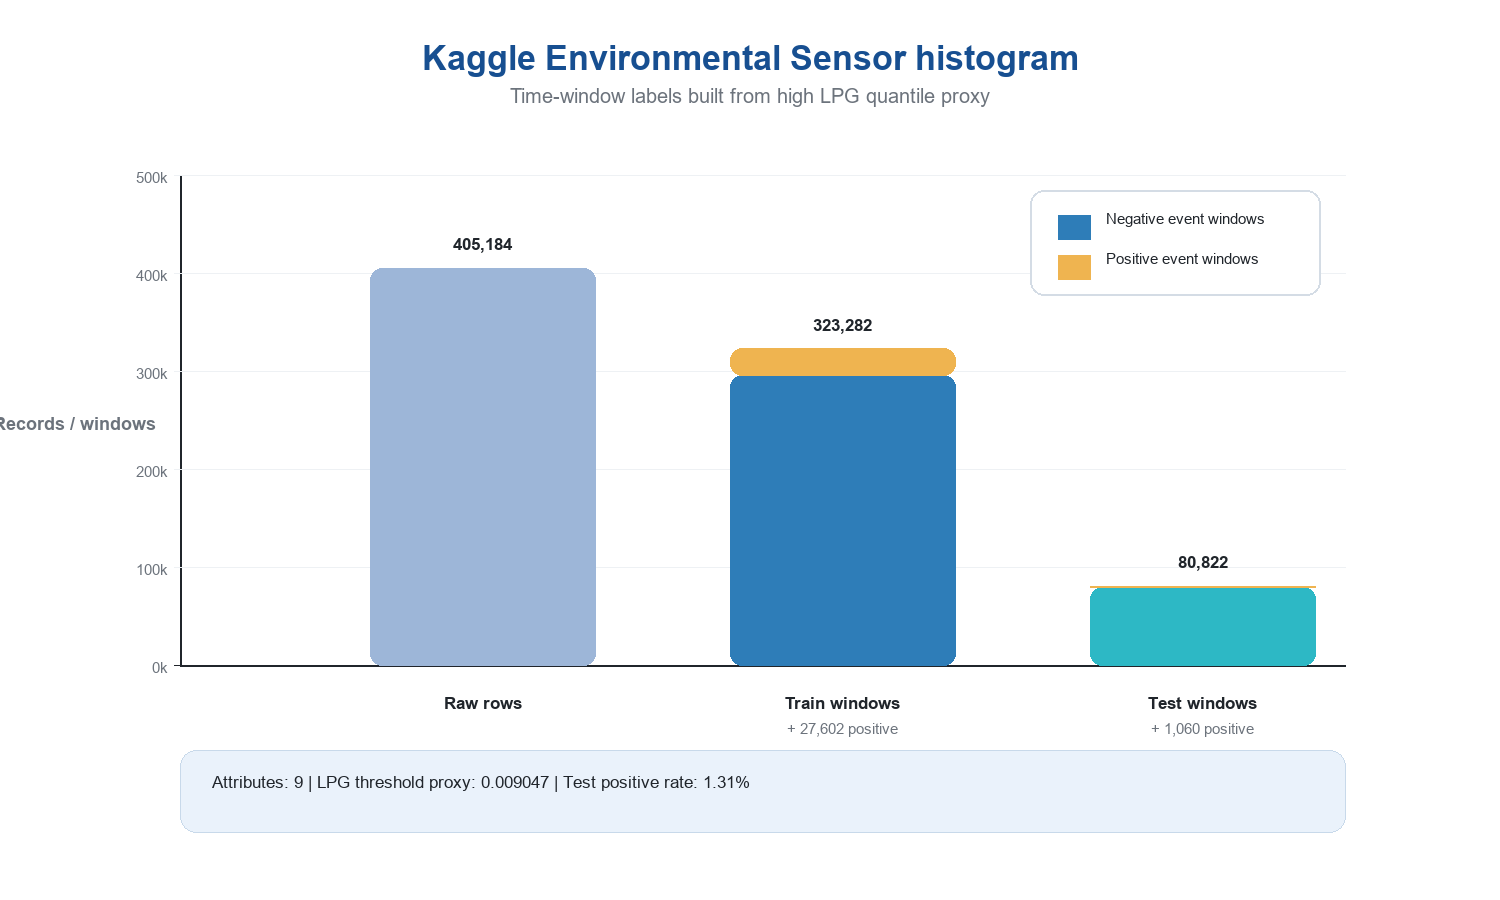
\includegraphics[width=0.95\linewidth]{exp/kaggle_dataset_histogram.png}
  \captionof{figure}{Histogram dữ liệu Kaggle sau khi chuyển thành cửa sổ chuỗi thời gian và nhãn sự kiện.}
  \label{fig:kaggle_dataset_histogram}
\end{center}

\subsection{Dữ liệu bộ mô phỏng}

Trong phạm vi đề tài, bộ mô phỏng được sử dụng để sinh dữ liệu mô phỏng và tạo môi trường thực nghiệm có kiểm soát. Dữ liệu mô phỏng không được xem là tập dữ liệu đã được chứng thực như các tập dữ liệu công khai UCI/Kaggle, mà là dữ liệu tổng hợp được sinh theo các quy tắc và kịch bản đã định nghĩa trước. Vai trò chính của bộ mô phỏng là:

\begin{itemize}
  \item Tạo dữ liệu huấn luyện có nhãn cho mô hình LSTM trong môi trường mô phỏng. Nhãn được sinh theo quy tắc dự báo, tức là kiểm tra xem nồng độ khí có vượt ngưỡng trong 5 phút tiếp theo hay không.
  
  \item Cung cấp môi trường tương tác cho bộ điều khiển PPO. Đây là vai trò quan trọng vì học tăng cường cần tác nhân thực hiện hành động và nhận phản hồi từ môi trường, trong khi các dataset log tĩnh như UCI/Kaggle không phản hồi lại hành động điều khiển.
  
  \item Tạo các testcase có kiểm soát như trạng thái bình thường, rò rỉ chậm, rò rỉ nhanh và thông gió để benchmark các bộ điều khiển.
  
  \item Kiểm thử luồng xử lý đầu cuối vì bộ mô phỏng gửi dữ liệu theo cùng cấu trúc JSON với thiết bị ESP32 dự kiến.
\end{itemize}

Nói cách khác, UCI/Kaggle nằm ở khối tham chiếu và kiểm chứng bổ sung trong giai đoạn phát triển mô hình, còn bộ mô phỏng nằm ở khối dữ liệu huấn luyện, bộ kiểm thử và môi trường tương tác cho PPO. Khi hệ thống vận hành, luồng xử lý không phân biệt dữ liệu đến từ ESP32 thật hay bộ mô phỏng, miễn là bản tin có cùng cấu trúc dữ liệu.

Hình~\ref{fig:sim_dataset_histogram} trực quan hóa phân bố dữ liệu mô phỏng được dùng để huấn luyện LSTM. Biểu đồ bên trái cho thấy phần lớn mẫu nằm ở vùng nền thấp, trong khi các mẫu vượt ngưỡng 1000\,ppm xuất hiện ít hơn và chủ yếu thuộc các pha rò rỉ. Biểu đồ bên phải cho thấy phân bố nhãn dự báo sự kiện: nhãn dương được gán khi cửa sổ hiện tại dẫn đến nguy cơ vượt ngưỡng trong 5 phút tiếp theo. Tỷ lệ mẫu dương khoảng 27{,}4\% cho thấy dữ liệu có mất cân bằng nhưng chưa đến mức cực đoan, vì vậy các chỉ số cảnh báo sau ngưỡng như Precision, Recall và F1-score cần được xem cùng Accuracy.

\Needspace{0.45\textheight}
\begin{center}
  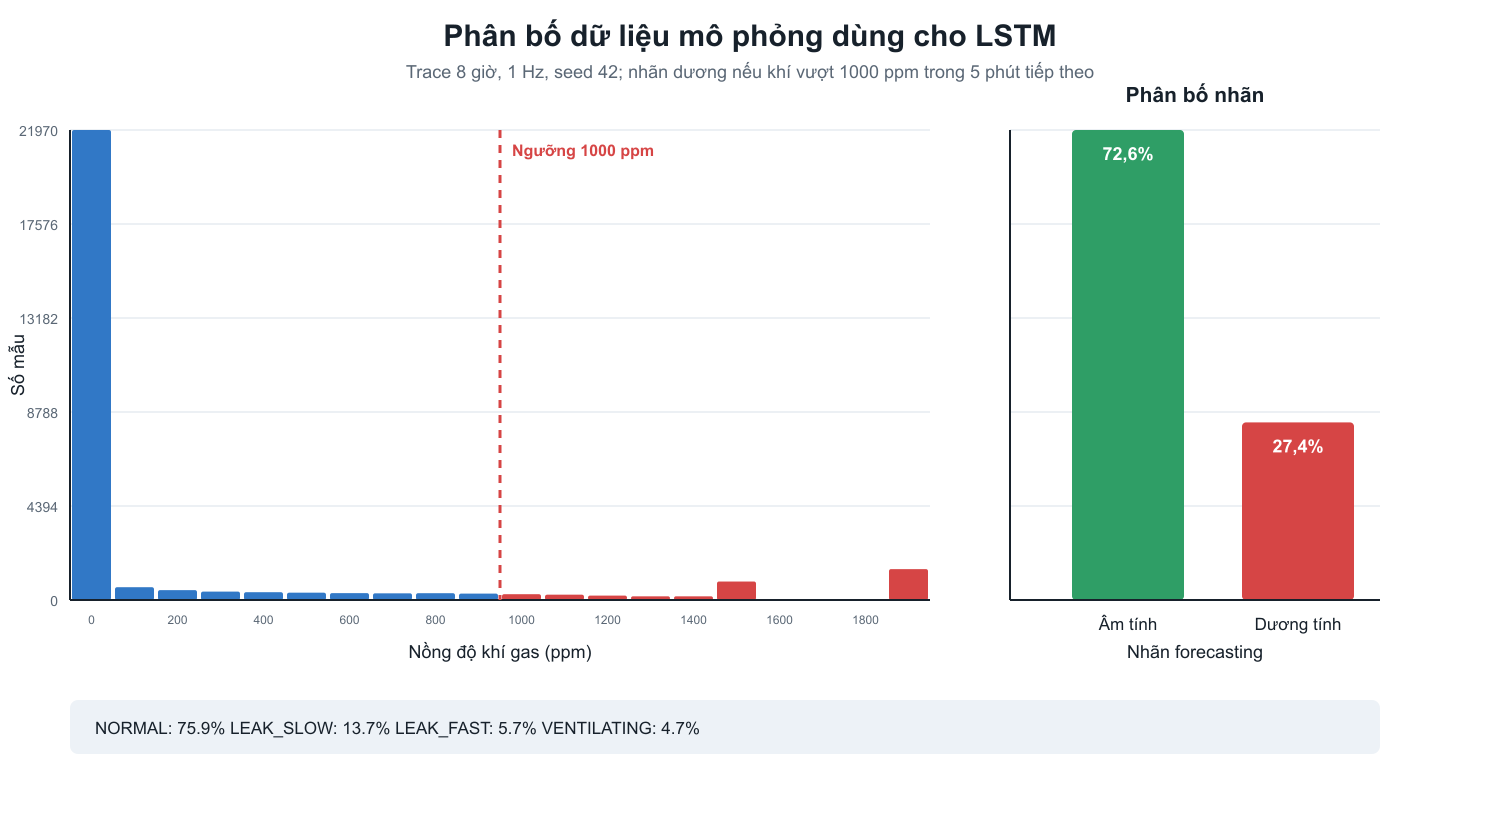
\includegraphics[width=1\linewidth]{exp/sim_dataset_histogram.png}
  \captionof{figure}{Histogram dữ liệu mô phỏng và phân bố nhãn dự báo sự kiện của LSTM.}
  \label{fig:sim_dataset_histogram}
\end{center}

\begingroup
\scriptsize
\renewcommand{\arraystretch}{1.18}
\setlength{\tabcolsep}{2.5pt}
\setlength{\LTleft}{0pt}
\setlength{\LTright}{0pt}

\begin{longtable}{
  >{\raggedright\arraybackslash}p{3.0cm}
  >{\raggedright\arraybackslash}p{3.5cm}
  >{\raggedright\arraybackslash}p{\dimexpr\textwidth-6.5cm-6\tabcolsep\relax}
}
\caption{Các trường dữ liệu chính trong thực nghiệm}
\label{tab:data_fields} \\
\toprule
\textbf{Trường dữ liệu} 
& \textbf{Ý nghĩa} 
& \textbf{Vai trò trong mô hình/hệ thống} \\
\midrule
\endfirsthead
\toprule
\textbf{Trường dữ liệu} 
& \textbf{Ý nghĩa} 
& \textbf{Vai trò trong mô hình/hệ thống} \\
\midrule
\endhead
\endfoot
\bottomrule
\endlastfoot

\texttt{device\_id} 
& Định danh thiết bị nguồn 
& Metadata, dùng để lọc dữ liệu theo thiết bị hoặc testcase. \\

\texttt{event\_ts} 
& Thời điểm phát sinh bản tin 
& Sắp xếp dữ liệu theo chuỗi thời gian và hỗ trợ tính độ trễ xử lý. \\

\texttt{gas\_ppm} 
& Nồng độ khí gas 
& Đầu vào của mô hình LSTM và là thành phần trạng thái của PPO. \\

\makecell[l]{\texttt{temperature\_}\\\texttt{c}}
& Nhiệt độ môi trường 
& Đầu vào cho LSTM và PPO để bổ sung ngữ cảnh môi trường. \\

\makecell[l]{\texttt{humidity\_}\\\texttt{percent}}
& Độ ẩm môi trường 
& Đầu vào cho LSTM và PPO để bổ sung ngữ cảnh môi trường. \\

\makecell[l]{\texttt{predicted\_risk}\\\texttt{\_5min}}
& Xác suất nguy hiểm trong 5 phút tiếp theo 
& Đầu ra của bộ dự báo LSTM và được dùng làm một thành phần đầu vào cho PPO. \\

\texttt{rl\_action} 
& Hành động điều khiển 
& Đầu ra của PPO, dùng để hiển thị trên bảng điều khiển và gửi sang Kafka action topic. \\

\end{longtable}
\endgroup

\section{Tiêu chí đánh giá}

Các tiêu chí đánh giá được lựa chọn nhằm phản ánh ba khía cạnh chính của hệ thống: khả năng dự báo của mô hình LSTM, hiệu quả điều khiển của PPO và độ tin cậy của pipeline dữ liệu. Bảng~\ref{tab:metrics} tổng hợp các tiêu chí được sử dụng trong quá trình thực nghiệm. Các công thức và ý nghĩa được trình bày tại đây để tránh lặp lại trong các phần đánh giá riêng phía sau.

\begingroup
\footnotesize
\renewcommand{\arraystretch}{1.28}
\setlength{\tabcolsep}{2pt}

% Kéo rộng bảng nhẹ sang hai bên để cột Ý nghĩa đỡ xuống dòng
\setlength{\LTleft}{-0.35cm}
\setlength{\LTright}{-0.35cm}

\begin{longtable}{
  >{\centering\arraybackslash}p{1.6cm}
  >{\raggedright\arraybackslash}p{3.0cm}
  >{\raggedright\arraybackslash}p{3.6cm}
  >{\raggedright\arraybackslash}p{\dimexpr\textwidth+0.7cm-1.6cm-3.0cm-3.6cm-8\tabcolsep\relax}
}
\caption{Tổng hợp các tiêu chí đánh giá}
\label{tab:metrics} \\
\toprule
\textbf{Nhóm} 
& \textbf{Tiêu chí} 
& \textbf{Công thức / cách tính} 
& \textbf{Ý nghĩa} \\
\midrule
\endfirsthead

% Không lặp lại header nếu bảng bị cắt sang trang mới
\endhead

% Không thêm dòng "Còn tiếp ở trang sau"
\endfoot

\bottomrule
\endlastfoot

\multirow{7}{*}{\textbf{LSTM}}
& \makecell[l]{\texttt{predicted\_risk}\\\texttt{\_5min}}
& $p_{5min} \in [0,1]$
& Chuỗi xác suất rủi ro do LSTM sinh ra theo từng cửa sổ trượt. Đây là đầu ra chính của bài toán time-series forecasting và được dùng làm đầu vào cho bộ điều khiển PPO. \\

& Binary cross-entropy
& $\displaystyle -\frac{1}{n}\sum_{i=1}^{n}\bigl[y_i\log(p_i)+(1-y_i)\log(1-p_i)\bigr]$
& Hàm mất mát huấn luyện cho bài toán dự báo sự kiện tương lai. Chỉ số này làm việc trực tiếp với xác suất $p_i$, chưa cần chuyển thành nhãn cứng. \\

& MAE sự kiện
& $\displaystyle \frac{1}{n}\sum_{i=1}^{n}|y_i-p_i|$
& Sai số tuyệt đối trung bình giữa nhãn sự kiện tương lai và xác suất dự báo. Tiêu chí này đo lỗi của sự kiện 0/1, không phải sai số nồng độ khí theo ppm. \\

& RMSE sự kiện
& $\displaystyle \sqrt{\frac{1}{n}\sum_{i=1}^{n}(y_i-p_i)^2}$
& Sai số bình phương trung bình trên xác suất dự báo sự kiện. Nếu mô hình đổi sang dự báo trực tiếp \texttt{gas\_ppm}, khi đó mới diễn giải RMSE theo đơn vị ppm. \\

& \makecell[l]{Confusion matrix\\(sau ngưỡng)}
& $\hat{y}_i=\mathbf{1}[p_i\geq\theta]$
& Chỉ dùng để kiểm tra tầng cảnh báo sau khi chuỗi xác suất được ngưỡng hóa, không phải metric chính của tầng time-series forecasting. \\

& \makecell[l]{Precision, Recall,\\F1-score}
& $\displaystyle P=\frac{TP}{TP+FP},\quad R=\frac{TP}{TP+FN}$
& Đánh giá chất lượng cảnh báo nhị phân sau ngưỡng. Recall quan trọng trong bài toán an toàn vì liên quan đến nguy cơ bỏ sót rò rỉ. \\

& Accuracy sau ngưỡng
& $\displaystyle \frac{TP+TN}{TP+TN+FP+FN}$
& Tỷ lệ quyết định cảnh báo đúng sau ngưỡng. Chỉ số này chỉ dùng kèm Precision/Recall vì dữ liệu có thể mất cân bằng. \\

\midrule

\multirow{5}{*}{\textbf{PPO}}
& \texttt{miss\_rate}
& $\displaystyle \frac{N_{\mathrm{miss}}}{N_{\mathrm{episode}}}$
& Tỷ lệ episode mà hệ thống để nồng độ khí chạm hoặc vượt ngưỡng nguy hiểm. Giá trị càng thấp cho thấy chính sách điều khiển càng an toàn. \\

& \texttt{peak\_gas}
& $\displaystyle \max_t gas_t$
& Nồng độ khí lớn nhất trong một episode. Chỉ số này phản ánh mức độ nghiêm trọng của tình huống sau khi bộ điều khiển can thiệp. \\

& Lead time
& $\displaystyle t_{\mathrm{threshold}} - t_{\mathrm{alert}}$
& Khoảng thời gian cảnh báo sớm trước khi nồng độ khí đạt ngưỡng nguy hiểm. Lead time càng lớn thì hệ thống càng có nhiều thời gian để phản ứng. \\

& \texttt{alarms/hour}
& $\displaystyle \frac{N_{\mathrm{alarm}}}{T_{\mathrm{hour}}}$
& Số cảnh báo trung bình trong một giờ. Chỉ số này dùng để đánh giá mức độ cảnh báo quá nhiều hoặc gây phiền nhiễu cho người dùng. \\

& Tỷ lệ can thiệp
& $\displaystyle \frac{N_{\mathrm{action}}}{N_{\mathrm{step}}}$
& Tỷ lệ bước thời gian mà bộ điều khiển chọn hành động can thiệp như cảnh báo, bật quạt hoặc đóng van. Chỉ số này phản ánh mức độ điều khiển quá mức. \\

\midrule

\multirow{4}{*}{\textbf{Pipeline}}
& Tỷ lệ truyền thành công
& $\displaystyle \frac{N_{\mathrm{received}}}{N_{\mathrm{sent}}}$
& Tỷ lệ bản tin được nhận và xử lý thành công so với số bản tin được gửi vào hệ thống. Tiêu chí này kiểm tra dữ liệu có đi qua đầy đủ các thành phần chính hay không. \\

& Throughput
& $\displaystyle \frac{N_{\mathrm{message}}}{T}$
& Số bản tin hệ thống xử lý được trong một đơn vị thời gian. Chỉ số này phản ánh khả năng đáp ứng khi dữ liệu tăng nhanh hoặc xuất hiện burst. \\

& Latency
& $\displaystyle t_{\mathrm{output}} - t_{\mathrm{input}}$
& Thời gian từ khi bản tin đi vào pipeline đến khi có kết quả xử lý hoặc hành động đầu ra. Độ trễ càng thấp thì hệ thống càng gần thời gian thực. \\

& Tỷ lệ phục hồi
& $\displaystyle \frac{N_{\mathrm{recovered}}}{N_{\mathrm{error}}}$
& Tỷ lệ trường hợp lỗi mà hệ thống vẫn tiếp tục chạy hoặc xử lý được sau khi gặp bản tin sai định dạng, lỗi tạm thời hoặc sự cố thành phần. \\

\end{longtable}
\endgroup

Trong đó, $p_i=p_{5min}(t_i)$ là xác suất rủi ro trong 5 phút tiếp theo tại cửa sổ thứ $i$, $y_i$ là nhãn sự kiện tương lai và $\hat{y}_i=\mathbf{1}[p_i\geq\theta]$ chỉ là quyết định cảnh báo sau ngưỡng. $TP$ là số mẫu nguy hiểm được cảnh báo đúng, $FP$ là số mẫu an toàn bị cảnh báo nhầm, $TN$ là số mẫu an toàn được dự đoán đúng và $FN$ là số mẫu nguy hiểm bị bỏ sót. Ký hiệu $N_{\mathrm{miss}}$ là số episode vượt ngưỡng nguy hiểm, $N_{\mathrm{episode}}$ là tổng số episode đánh giá, $N_{\mathrm{alarm}}$ là số lần cảnh báo, $T_{\mathrm{hour}}$ là thời gian đánh giá tính theo giờ, $N_{\mathrm{sent}}$ và $N_{\mathrm{received}}$ lần lượt là số bản tin gửi vào và nhận được ở đầu ra của pipeline.

\section{Kết quả huấn luyện mô hình}
\label{sec:model_training_results}

Phần này trình bày kết quả huấn luyện và kiểm chứng hai mô hình chính của hệ thống: bộ dự báo LSTM và bộ điều khiển PPO. LSTM được đánh giá theo khả năng dự báo sự kiện nguy hiểm trong tương lai gần, trong khi PPO được đánh giá thông qua quá trình học chính sách điều khiển trong môi trường mô phỏng.

\subsection{Kết quả huấn luyện và kiểm chứng LSTM}
\label{sec:lstm_eval}

\subsubsection{Bài toán và cấu hình mô hình}

Mô hình LSTM được sử dụng để dự báo nguy cơ nồng độ khí vượt ngưỡng trong tương lai gần. Đầu vào của mô hình là một cửa sổ chuỗi thời gian gồm 60 mẫu gần nhất, với ba đặc trưng cảm biến chính:

\[
X_t = [gas\_ppm, temperature\_c, humidity\_percent]_{t-59:t}.
\]

Đầu ra của mô hình là một giá trị xác suất trong khoảng $[0,1]$, ký hiệu là $p_{5min}$. Giá trị này biểu diễn khả năng nồng độ khí sẽ vượt ngưỡng 1000\,ppm trong 5 phút tiếp theo:

\[
p_{5min} = P\left(\max_{t < \tau \leq t+300} gas_\tau > 1000\,ppm\right).
\]

Khi hệ thống chạy liên tục, mỗi cửa sổ trượt sinh ra một giá trị $p_{5min}(t)$, tạo thành chuỗi \texttt{predicted\_risk\_5min} theo thời gian. Như vậy, LSTM không chỉ phân loại trạng thái hiện tại của môi trường, mà thực hiện bài toán \emph{dự báo nguy cơ trong tương lai}. Classification chỉ xuất hiện ở bước sau, khi chuỗi xác suất này được so với một ngưỡng để tạo cảnh báo nhị phân.

\subsubsection{Tiêu chí đánh giá LSTM}

Đầu ra của LSTM là xác suất của một sự kiện tương lai, không phải nhãn trạng thái hiện tại. Vì vậy, phần đánh giá được tách thành hai tầng. Ở tầng time-series forecasting, chuỗi $p_{5min}(t)$ thể hiện xu hướng rủi ro theo thời gian và được đánh giá bằng loss/MAE/RMSE trên biến sự kiện tương lai. Ở tầng alert/classification, sau khi chọn ngưỡng quyết định, xác suất này mới được chuyển thành cảnh báo nhị phân để tính Accuracy, Precision, Recall, F1-score và confusion matrix. Nói cách khác, confusion matrix không thay thế đánh giá time-series; nó chỉ trả lời câu hỏi nếu dùng ngưỡng $\theta$ thì hệ thống cảnh báo đúng/sai như thế nào. Nếu đổi mục tiêu thành dự báo trực tiếp giá trị nồng độ khí liên tục, khi đó mới cần MAE/RMSE theo đơn vị ppm.

\Needspace{0.42\textheight}
\begin{center}
  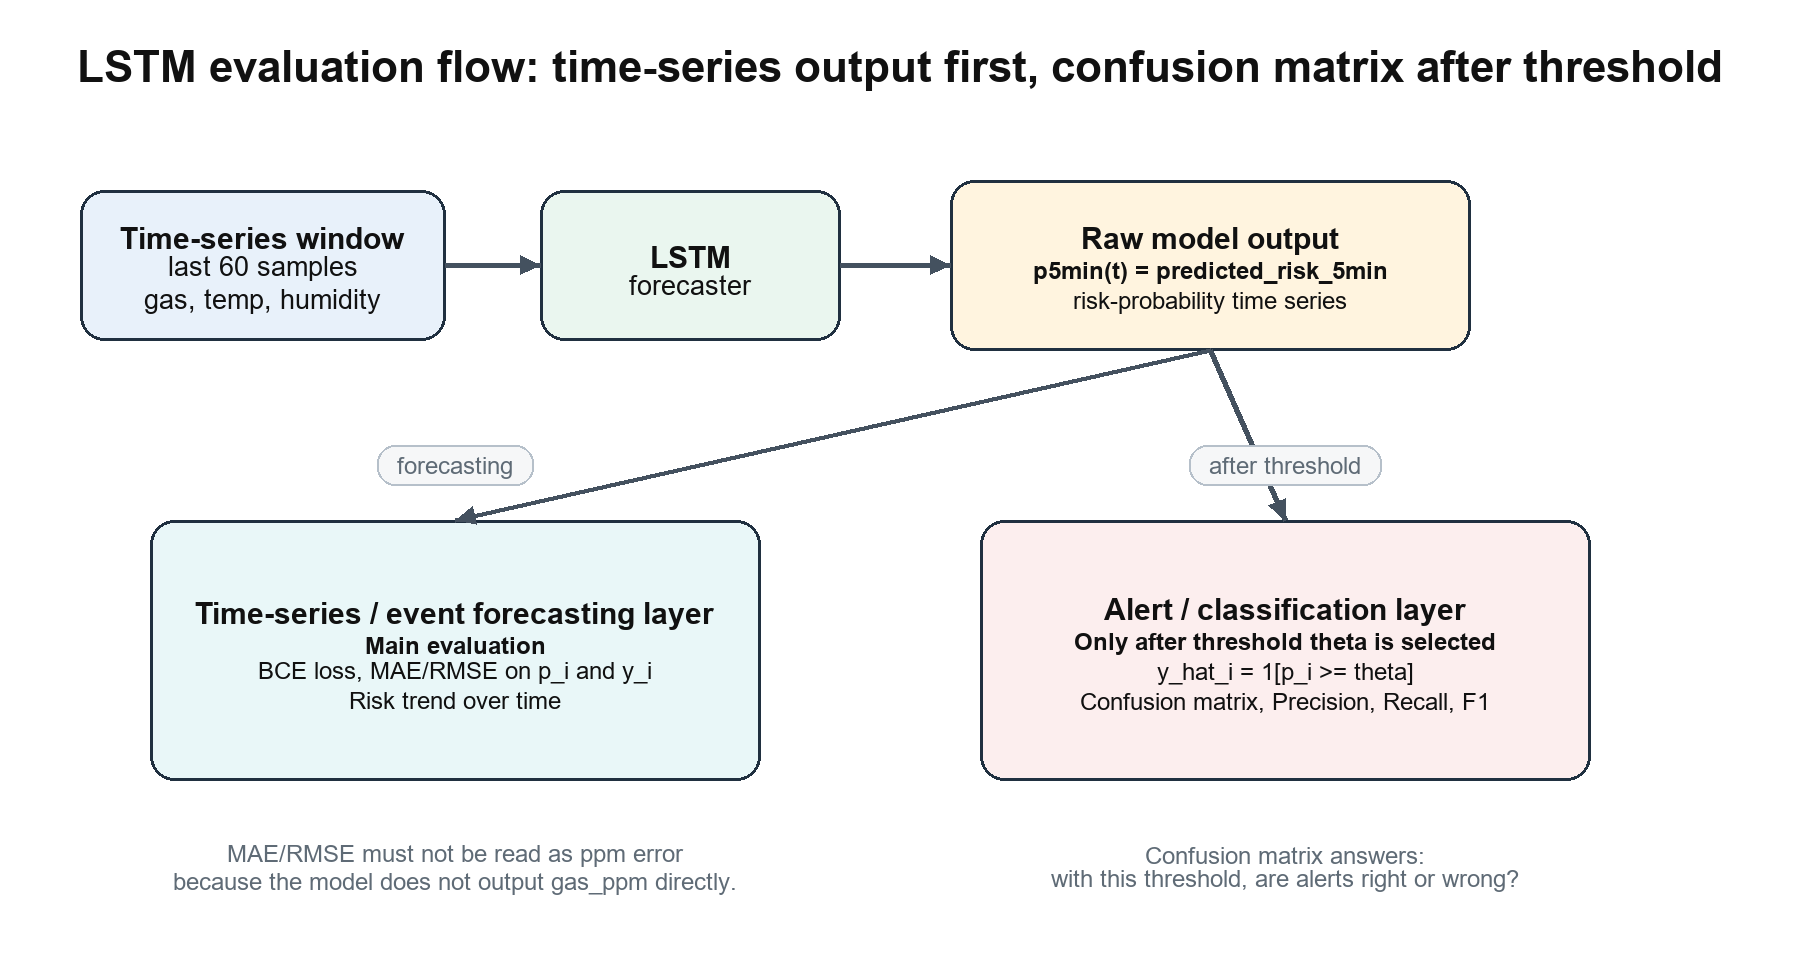
\includegraphics[width=0.95\linewidth]{exp/lstm_evaluation_flow.png}
  \captionof{figure}{Sơ đồ tách tầng đánh giá LSTM giữa time-series forecasting và alert/classification sau ngưỡng.}
  \label{fig:lstm_evaluation_flow}
\end{center}

\subsubsection{Kết quả trên trace mô phỏng}

Trace mô phỏng được sử dụng để đánh giá khả năng dự báo sự kiện trong môi trường có nhãn thật rõ ràng. Kết quả từ file \texttt{lstm\_metrics.json} được tổng hợp trong Bảng~\ref{tab:lstm_metrics}.

\begingroup
\small
\renewcommand{\arraystretch}{1.25}
\setlength{\tabcolsep}{5pt}
\setlength{\LTleft}{\fill}
\setlength{\LTright}{\fill}

\begin{longtable}{lc}
\caption{Kết quả đánh giá LSTM trên tập kiểm thử mô phỏng}
\label{tab:lstm_metrics} \\
\toprule
\textbf{Chỉ số} & \textbf{Giá trị} \\
\midrule
\endfirsthead
\toprule
\textbf{Chỉ số} & \textbf{Giá trị} \\
\midrule
\endhead
\endfoot
\bottomrule
\endlastfoot
Train windows & 22{,}752 \\
Test windows & 5{,}688 \\
Input window & 60 mẫu \\
Forecast horizon & 300\,s \\
Epochs & 20 \\
Positive rate toàn bộ & 27{,}43\% \\
Accuracy sau ngưỡng & 90{,}51\% \\
Precision sau ngưỡng & 100{,}00\% \\
Recall sau ngưỡng & 55{,}15\% \\
F1-score sau ngưỡng & 71{,}09\% \\
TP / FP / TN / FN & 664 / 0 / 4{,}484 / 540 \\
\end{longtable}
\endgroup

Trong huấn luyện LSTM, một \textit{epoch} là một lượt mô hình đi qua toàn bộ tập train một lần. Số epoch không phải đầu ra của hệ thống, mà là tham số huấn luyện dùng để theo dõi mô hình đã học đủ hay chưa, loss có hội tụ không và có dấu hiệu overfit trên validation hay không. Trong thí nghiệm này, mô hình được huấn luyện 20 epochs theo cấu hình trong script \texttt{train\_forecaster\_colab.py}; sau mỗi epoch, Keras ghi lại \texttt{loss}, \texttt{val\_loss}, \texttt{accuracy}, \texttt{precision} và \texttt{recall} vào biến \texttt{history.history}.

Hình~\ref{fig:lstm_epoch_metrics} là biểu đồ huấn luyện LSTM theo epoch. Loss huấn luyện giảm dần, cho thấy mô hình học được quy luật từ chuỗi cảm biến. Các đường accuracy, Precision và Recall trong hình là chỉ số theo dõi phụ sau ngưỡng 0{,}5 do Keras ghi lại trong lúc train; chúng giúp quan sát hành vi cảnh báo nhị phân, nhưng không thay thế đánh giá chuỗi xác suất $p_{5min}(t)$. Validation loss và validation Precision có dao động do dữ liệu được chia theo thứ tự thời gian và các pha rò rỉ không phân bố đều giữa các đoạn.

\Needspace{0.55\textheight}
\begin{center}
  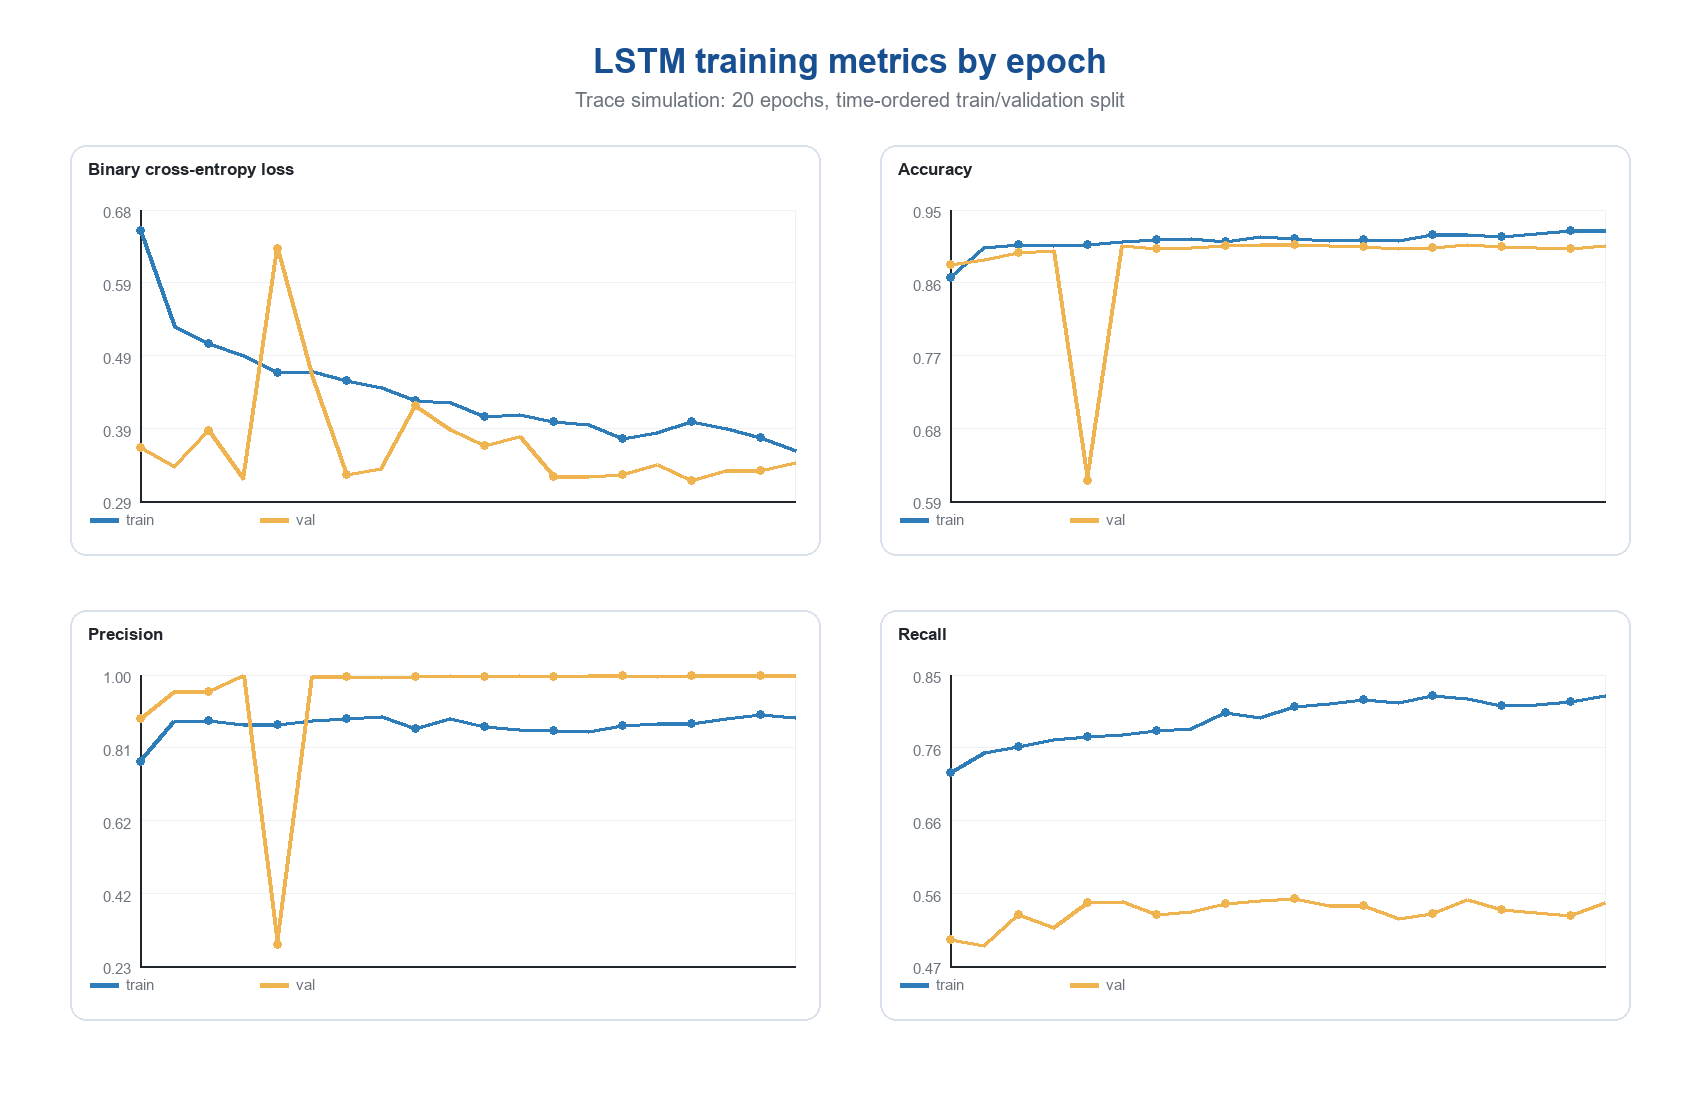
\includegraphics[width=1\linewidth]{exp/lstm_epoch_metrics.png}
  \captionof{figure}{Biểu đồ huấn luyện LSTM theo epoch: loss và các chỉ số cảnh báo sau ngưỡng.}
  \label{fig:lstm_epoch_metrics}
\end{center}

Kết quả cho thấy mô hình LSTM có xu hướng dự báo thận trọng. Precision đạt 100\%, nghĩa là trên tập kiểm thử mô phỏng, khi mô hình dự đoán nguy hiểm thì không có cảnh báo sai. Tuy nhiên, Recall chỉ đạt 55{,}15\%, cho thấy mô hình còn bỏ sót một phần các cửa sổ nguy hiểm. Nguyên nhân có thể đến từ các giai đoạn đầu của rò rỉ chậm, khi nồng độ khí chưa tăng đủ rõ trong cửa sổ 60 mẫu.

Trong bài toán an toàn, Recall có vai trò đặc biệt quan trọng vì bỏ sót nguy cơ rò rỉ có thể gây hậu quả nghiêm trọng. Do đó, ngưỡng quyết định của mô hình có thể được điều chỉnh thấp hơn để tăng Recall, sau đó tầng điều khiển PPO sẽ quyết định hành động phù hợp dựa trên xác suất rủi ro liên tục thay vì chỉ dựa vào nhãn nhị phân.

Ma trận nhầm lẫn ở Hình~\ref{fig:lstm_confusion} chỉ được dùng như kiểm tra phụ cho tầng cảnh báo sau ngưỡng. Phần này không xem confusion matrix là metric chính của LSTM, vì đầu ra gốc của mô hình vẫn là chuỗi xác suất \texttt{predicted\_risk\_5min}.

\Needspace{0.34\textheight}
\begin{center}
  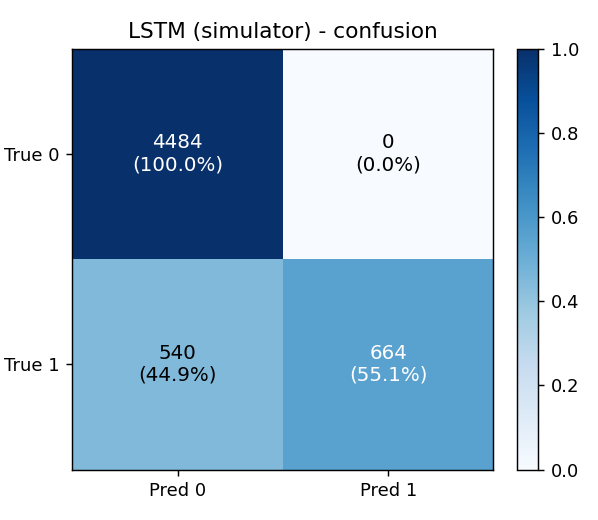
\includegraphics[width=0.62\linewidth]{exp/lstm_confusion_matrix.png}
  \captionof{figure}{Ma trận nhầm lẫn sau ngưỡng của LSTM trên tập kiểm thử mô phỏng.}
  \label{fig:lstm_confusion}
\end{center}

Hình~\ref{fig:lstm_threshold_tradeoff} cho thấy khi giảm ngưỡng quyết định từ 0{,}5 xuống 0{,}2, Recall tăng lên khoảng 82{,}9\% nhưng Precision giảm xuống khoảng 64{,}4\%. Trong bài toán an toàn, lựa chọn ngưỡng thấp hơn có thể hợp lý hơn vì chi phí bỏ sót nguy hiểm thường lớn hơn chi phí cảnh báo sớm. Tuy nhiên, ngưỡng này cần được hiệu chỉnh tiếp khi có dữ liệu cảm biến thực.

\Needspace{0.45\textheight}
\begin{center}
  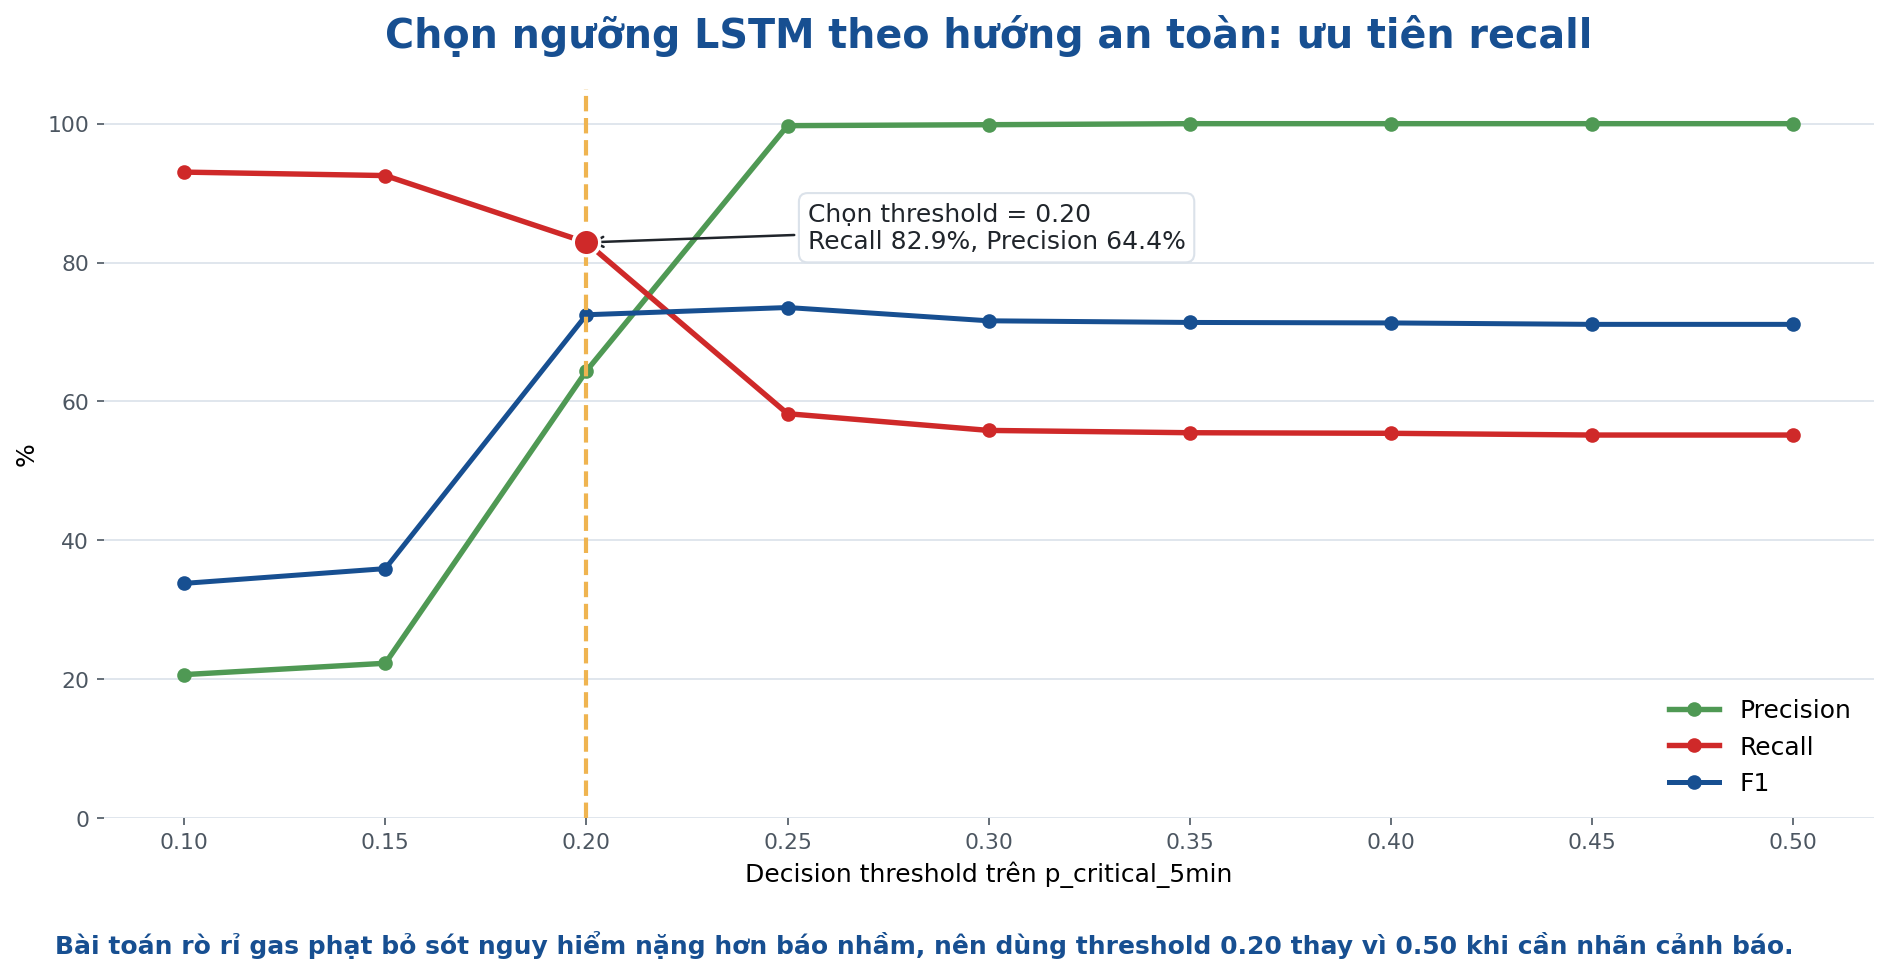
\includegraphics[width=0.95\linewidth]{exp/lstm_threshold_tradeoff.png}
  \captionof{figure}{Quan hệ giữa Precision, Recall và F1-score theo ngưỡng quyết định của LSTM.}
  \label{fig:lstm_threshold_tradeoff}
\end{center}

\subsubsection{Kiểm chứng trên dữ liệu cảm biến công khai}

Để tránh chỉ đánh giá trên dữ liệu mô phỏng, đề tài thực hiện kiểm chứng bổ sung trên tập dữ liệu cảm biến IoT công khai \texttt{environmental-sensor-data-132k} từ Kaggle~\cite{stafford2020envsensor}. Tập dữ liệu này chứa các tín hiệu LPG, CO, smoke, nhiệt độ và độ ẩm từ các thiết bị IoT. Tuy nhiên, tập dữ liệu không có nhãn rò rỉ LPG thật, vì vậy nhãn dương được xây dựng theo quy tắc gần đúng, dựa trên ngưỡng phân vị cao của tín hiệu LPG.

Do đó, kết quả trên tập Kaggle chỉ được dùng để đánh giá sơ bộ khả năng học xu hướng tín hiệu cảm biến của mô hình LSTM, không được dùng để khẳng định khả năng phát hiện rò rỉ LPG an toàn trong môi trường thực tế.

\begingroup
\small
\renewcommand{\arraystretch}{1.25}
\setlength{\tabcolsep}{5pt}

\begin{longtable}{
  >{\raggedright\arraybackslash}p{6.2cm}
  >{\centering\arraybackslash}p{5.0cm}
}
\caption{Kết quả LSTM trên tập dữ liệu cảm biến công khai Kaggle}
\label{tab:lstm_metrics_kaggle} \\
\toprule
\textbf{Chỉ số} 
& \textbf{Giá trị} \\
\midrule
\endfirsthead

% Không lặp lại header nếu bảng bị cắt sang trang mới
\endhead

% Không thêm dòng "Còn tiếp ở trang sau"
\endfoot

\bottomrule
\endlastfoot

Train windows 
& 323{,}282 \\

Test windows 
& 80{,}822 \\

Positive rate test 
& 1{,}31\% \\

Accuracy sau ngưỡng
& 96{,}36\% \\

Precision sau ngưỡng
& 25{,}54\% \\

Recall sau ngưỡng
& 92{,}83\% \\

F1-score sau ngưỡng
& 40{,}06\% \\

TP / FP / TN / FN 
& 984 / 2{,}869 / 76{,}893 / 76 \\

\end{longtable}
\endgroup

Kết quả trên Kaggle cho thấy Recall đạt 92{,}83\%, tức là mô hình phát hiện được phần lớn các trường hợp tín hiệu LPG cao trong tương lai theo nhãn proxy. Tuy nhiên, Precision chỉ đạt 25{,}54\%, phản ánh số cảnh báo nhầm còn cao. Điều này là hợp lý vì nhãn trên tập Kaggle không phải nhãn rò rỉ thật, mà chỉ là nhãn gần đúng được xây dựng từ phân vị của tín hiệu LPG. Ngoài ra, dữ liệu cảm biến thực thường có nhiễu, dao động ngắn hạn và sự khác biệt giữa các thiết bị.

Tương tự trace mô phỏng, ma trận nhầm lẫn trên Kaggle chỉ mô tả kết quả sau khi ngưỡng hóa xác suất dự báo. Do nhãn Kaggle là nhãn proxy, hình này được dùng để quan sát xu hướng lỗi cảnh báo, không dùng để kết luận rằng mô hình đã được chứng nhận phát hiện rò rỉ thật.

\Needspace{0.4\textheight}
\begin{center}
  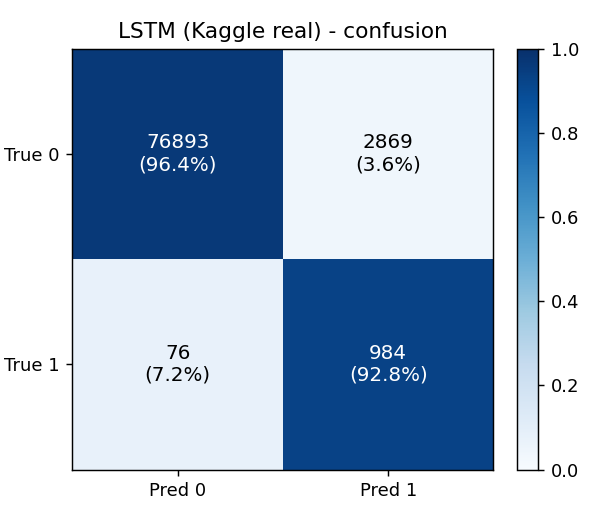
\includegraphics[width=0.62\linewidth]{exp/lstm_confusion_matrix_kaggle.png}
  \captionof{figure}{Ma trận nhầm lẫn sau ngưỡng của LSTM trên dữ liệu cảm biến công khai.}
  \label{fig:lstm_confusion_kaggle}
\end{center}

\subsubsection{So sánh kết quả giữa dữ liệu mô phỏng và dữ liệu công khai}

Bảng~\ref{tab:lstm_compare_results} tổng hợp kết quả LSTM trên hai nguồn dữ liệu. Mục tiêu của bảng này là làm rõ sự khác biệt giữa dữ liệu mô phỏng có ground-truth rõ ràng và dữ liệu cảm biến công khai có nhãn proxy.

\begingroup
\small
\renewcommand{\arraystretch}{1.25}
\setlength{\tabcolsep}{5pt}
\setlength{\LTleft}{0pt}
\setlength{\LTright}{0pt}

\begin{longtable}{
  >{\raggedright\arraybackslash}p{3.2cm}
  >{\centering\arraybackslash}p{3.2cm}
  >{\centering\arraybackslash}p{3.2cm}
  >{\raggedright\arraybackslash}p{\dimexpr\textwidth-9.6cm-8\tabcolsep\relax}
}
\caption{So sánh kết quả LSTM trên dữ liệu mô phỏng và dữ liệu công khai}
\label{tab:lstm_compare_results} \\
\toprule
\textbf{Chỉ số} 
& \textbf{Trace mô phỏng} 
& \textbf{Kaggle} 
& \textbf{Nhận xét} \\
\midrule
\endfirsthead
\toprule
\textbf{Chỉ số} 
& \textbf{Trace mô phỏng} 
& \textbf{Kaggle} 
& \textbf{Nhận xét} \\
\midrule
\endhead
\endfoot
\bottomrule
\endlastfoot

Accuracy sau ngưỡng
& 90{,}51\% 
& 96{,}36\% 
& Kaggle có Accuracy cao, nhưng cần lưu ý tập test có tỷ lệ mẫu dương thấp. \\

Precision sau ngưỡng
& 100{,}00\% 
& 25{,}54\% 
& Mô phỏng có ít cảnh báo sai hơn; Kaggle có nhiều cảnh báo nhầm do nhãn proxy và nhiễu cảm biến. \\

Recall sau ngưỡng
& 55{,}15\% 
& 92{,}83\% 
& Kaggle đạt Recall cao, cho thấy mô hình bắt được nhiều trường hợp tín hiệu LPG cao trong tương lai. \\

F1-score sau ngưỡng
& 71{,}09\% 
& 40{,}06\% 
& F1 trên Kaggle thấp hơn do Precision thấp. \\

TP / FP / TN / FN 
& 664 / 0 / 4{,}484 / 540 
& 984 / 2{,}869 / 76{,}893 / 76 
& Phân bố lỗi khác nhau giữa dữ liệu mô phỏng và dữ liệu cảm biến công khai. \\

\end{longtable}
\endgroup

Hình~\ref{fig:lstm_mae_rmse} bổ sung MAE/RMSE cho lỗi sự kiện. Về nguyên tắc, MAE/RMSE nên được tính trực tiếp trên xác suất $p_{5min}(t)$ và nhãn sự kiện tương lai $y_t$. Với các kết quả đã lưu chỉ gồm TP/FP/TN/FN, hình này dùng cách xấp xỉ sau ngưỡng để minh họa mức lỗi sự kiện của hai tập dữ liệu; do đó không được diễn giải là sai số dự báo nồng độ khí theo ppm vì mô hình hiện tại không xuất trực tiếp $\hat{gas}_{t+h}$.

\Needspace{0.45\textheight}
\begin{center}
  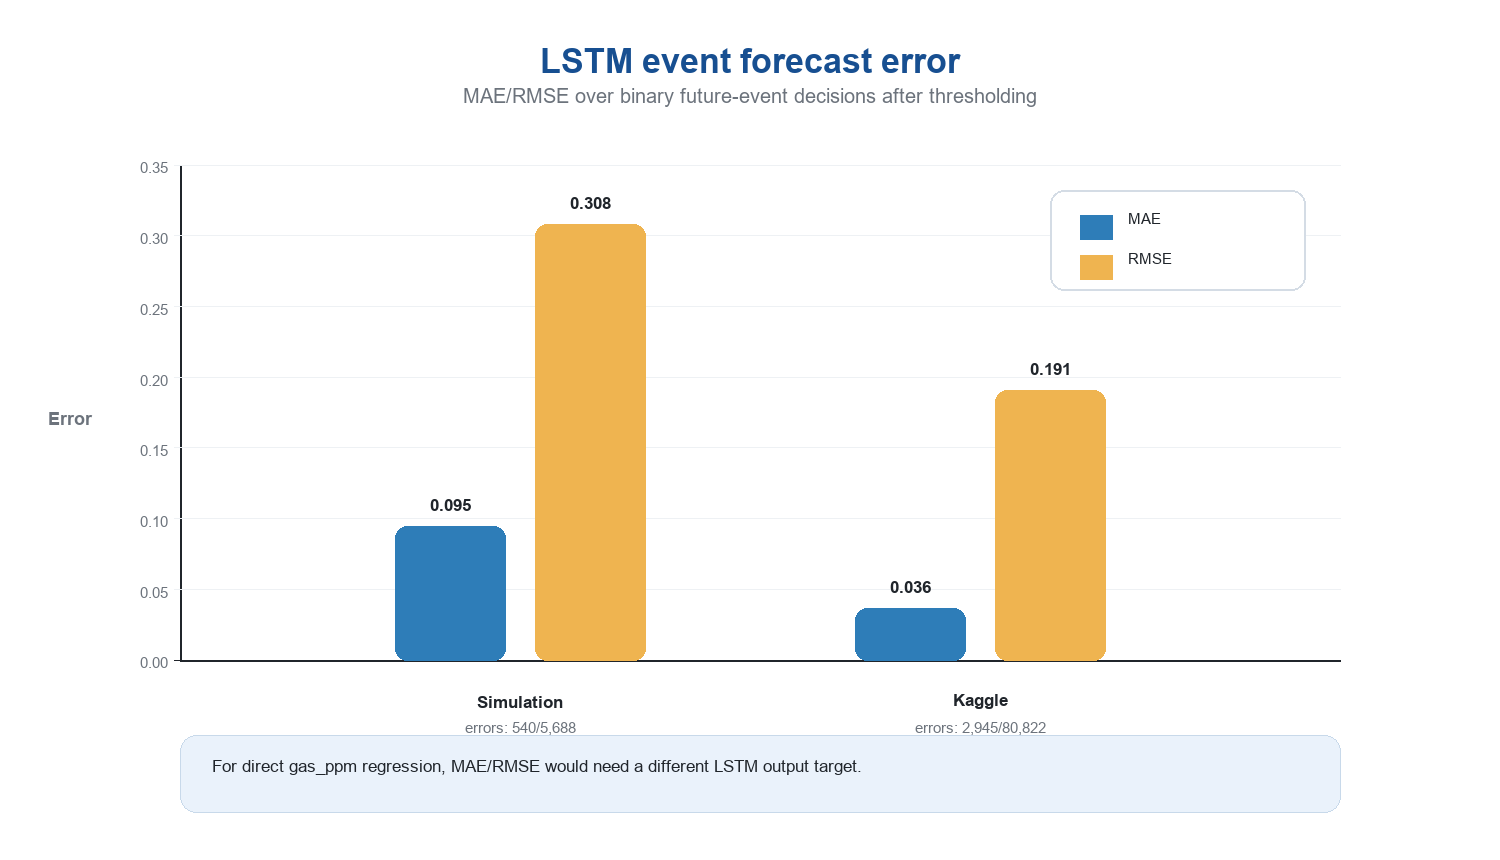
\includegraphics[width=0.92\linewidth]{exp/lstm_mae_rmse.png}
  \captionof{figure}{MAE/RMSE xấp xỉ của LSTM trên lỗi sự kiện ở dữ liệu mô phỏng và Kaggle.}
  \label{fig:lstm_mae_rmse}
\end{center}

\subsubsection{Nhận xét về mô hình LSTM}

Từ các kết quả trên, LSTM cho thấy vai trò phù hợp trong việc dự báo xu hướng rủi ro của nồng độ khí. Mô hình không thay thế các ngưỡng an toàn vật lý, mà đóng vai trò cung cấp thêm tín hiệu cảnh báo sớm cho bộ điều khiển.

Trong hệ thống triển khai, đầu ra của LSTM được biểu diễn bằng trường \texttt{predicted\_risk\_5min} và được đưa vào PPO như một phần của trạng thái quan sát. Nhờ đó, PPO có thể cân nhắc cả nồng độ khí hiện tại lẫn khả năng rủi ro trong vài phút tiếp theo trước khi lựa chọn hành động điều khiển.

\subsection{Kết quả huấn luyện PPO}
\label{sec:ppo_training_results}

\subsubsection{Thiết lập huấn luyện PPO}

Bộ điều khiển PPO được đánh giá trong môi trường \texttt{GasLeakEnv} đã được mô tả ở Chương~3. Phần này sẽ tập trung vào kết quả sau huấn luyện của chính sách PPO.

Mục tiêu đánh giá là kiểm tra liệu PPO có giữ nồng độ khí dưới ngưỡng nguy hiểm, phản ứng đủ sớm trong các kịch bản rò rỉ và hạn chế cảnh báo hoặc can thiệp không cần thiết hay không. Các tiêu chí sử dụng gồm \texttt{miss\_rate}, \texttt{peak\_gas}, lead time, \texttt{alarms/hour} và tỷ lệ can thiệp; ý nghĩa và công thức đã được trình bày trong Bảng~\ref{tab:metrics}.

Reward của \texttt{GasLeakEnv} được sử dụng theo cấu hình đã trình bày ở Chương~3. Trong Chương~4, reward chỉ được dùng để quan sát quá trình học và mức độ hội tụ của tác nhân. Việc kết luận hiệu quả điều khiển vẫn dựa chủ yếu trên các chỉ số đánh giá trực tiếp như \texttt{miss\_rate}, \texttt{peak\_gas} và \texttt{alarms/hour}.

\subsubsection{Hội tụ trong quá trình huấn luyện}

Đường cong phần thưởng huấn luyện được trình bày ở Hình~\ref{fig:ppo_reward}. Ở giai đoạn đầu, phần thưởng trung bình rất thấp do tác nhân còn khám phá ngẫu nhiên và thường để khí vượt ngưỡng. Sau khoảng vài chục nghìn bước thời gian, phần thưởng trung bình tăng nhanh về gần vùng ổn định. Về cuối quá trình huấn luyện, phần thưởng dao động quanh vùng gần 0 với một số episode âm sâu do môi trường vẫn có các pha rò rỉ nhanh khó kiểm soát hoặc do hành động khám phá. Như vậy, PPO có dấu hiệu hội tụ về một chính sách ổn định trong môi trường mô phỏng, nhưng kết luận này vẫn cần được kiểm chứng thêm bằng nhiều seed và nhiều kịch bản khi triển khai phần cứng.

\Needspace{0.45\textheight}
\begin{center}
  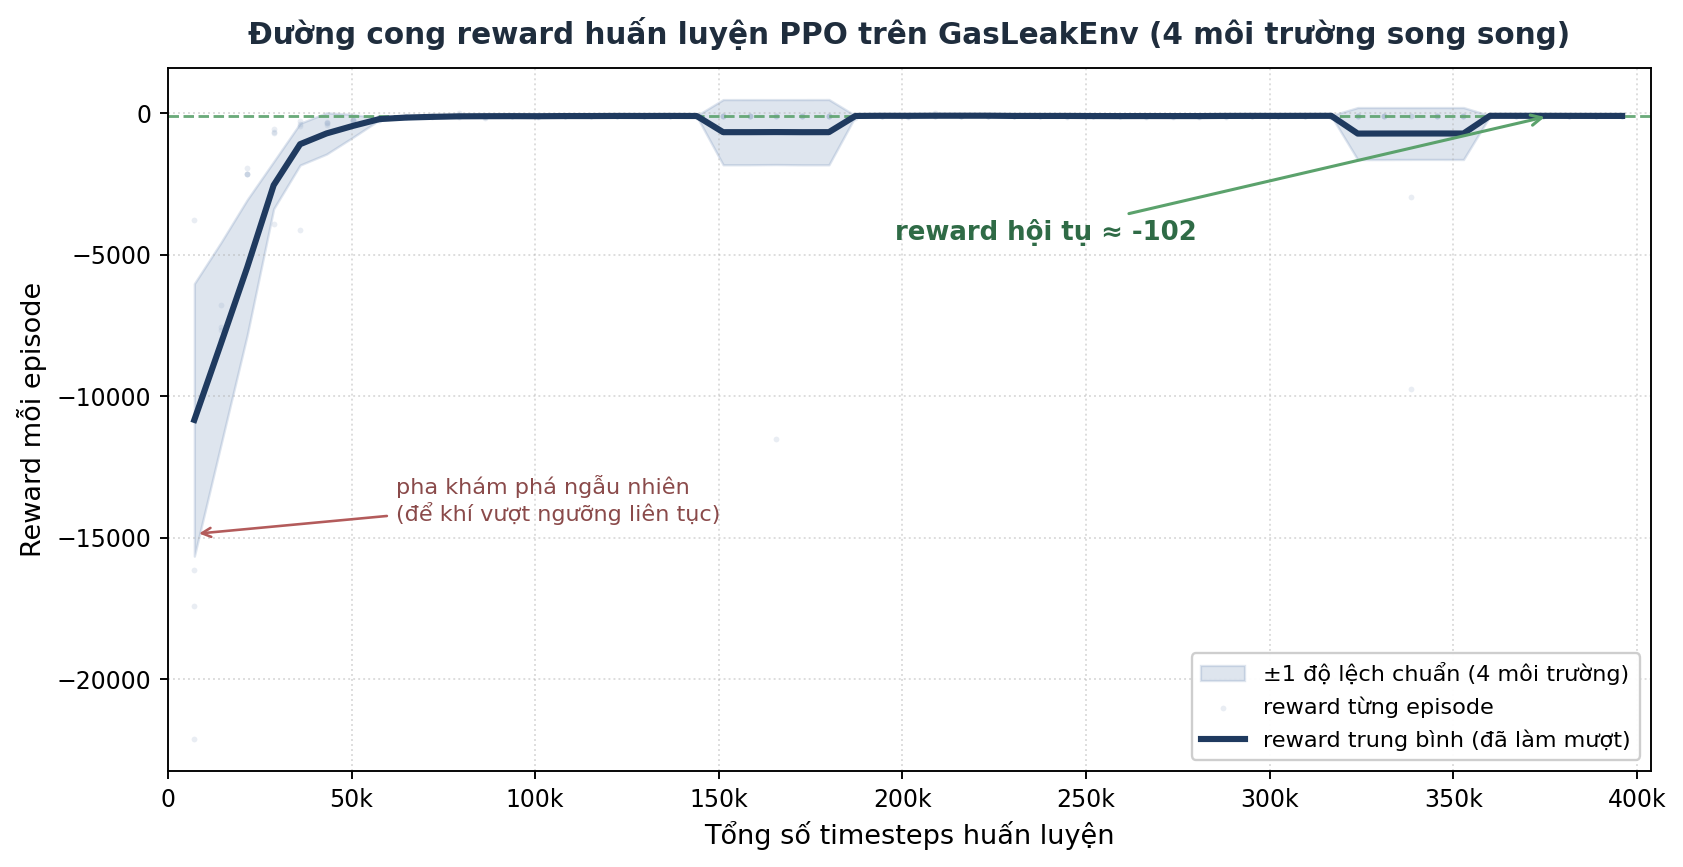
\includegraphics[width=0.95\linewidth]{exp/ppo_reward.png}
  \captionof{figure}{Đường cong reward trong quá trình huấn luyện PPO.}
  \label{fig:ppo_reward}
\end{center}

\section{Các kịch bản đánh giá}
\label{sec:evaluation_scenarios}

Sau khi huấn luyện mô hình, hệ thống được đánh giá qua nhiều nhóm kịch bản nhằm kiểm tra khả năng vận hành trong các điều kiện khác nhau. Các kịch bản được chia thành năm nhóm: benchmark bộ điều khiển, kịch bản rò rỉ chậm/rò rỉ nhanh, testcase vận hành LSTM/PPO, testcase pipeline dữ liệu và độ trễ suy luận.

\subsection{Tổng quan các nhóm kịch bản}

\begingroup
\small
\renewcommand{\arraystretch}{1.25}
\setlength{\tabcolsep}{3pt}

% Kéo rộng bảng nhẹ sang hai bên để nội dung ít bị xuống dòng
\setlength{\LTleft}{-0.25cm}
\setlength{\LTright}{-0.25cm}

\begin{longtable}{
  >{\raggedright\arraybackslash}p{3.0cm}
  >{\raggedright\arraybackslash}p{4.0cm}
  >{\raggedright\arraybackslash}p{\dimexpr\textwidth+0.5cm-3.0cm-4.0cm-6\tabcolsep\relax}
}
\caption{Tổng quan các nhóm kịch bản đánh giá}
\label{tab:evaluation_scenario_groups} \\
\toprule
\textbf{Nhóm kịch bản} 
& \textbf{Mục tiêu} 
& \textbf{Nội dung đánh giá} \\
\midrule
\endfirsthead

% Không lặp lại header nếu bảng bị cắt sang trang mới
\endhead

% Không thêm dòng "Còn tiếp ở trang sau"
\endfoot

\bottomrule
\endlastfoot

Benchmark bộ điều khiển
& So sánh PPO với các phương pháp cơ sở.
& Đánh giá \textbf{THRESHOLD}, \textbf{FORECASTER}, \textbf{RULE}, \textbf{PPO} và thí nghiệm ablation \textbf{PPO-only}/\textbf{LSTM+PPO} theo \texttt{miss\_rate}, \texttt{alarms/hour} và \texttt{peak\_gas}. \\

Kịch bản rò rỉ đơn
& Quan sát phản ứng trong hai tình huống rò rỉ đặc trưng.
& Đánh giá rò rỉ chậm và rò rỉ nhanh thông qua lead time, peak gas và khả năng giữ khí dưới ngưỡng nguy hiểm. \\

Testcase vận hành LSTM/PPO
& Kiểm tra hành vi hệ thống trên dashboard và kênh cảnh báo.
& Đánh giá các testcase TC1--TC4 gồm trạng thái bình thường, nấu ăn/phòng kín, rò rỉ nguy hiểm và phục hồi sau điều khiển. \\

Testcase pipeline dữ liệu
& Kiểm tra luồng dữ liệu đầu cuối.
& Đánh giá MQTT--Kafka--Spark--database với dữ liệu bình thường, tải trung bình, burst, nhiều topic và dữ liệu lỗi. \\

Độ trễ suy luận
& Đánh giá khả năng đáp ứng của mô hình.
& Đo thời gian suy luận của LSTM và PPO để xác định thành phần có khả năng ảnh hưởng đến xử lý gần thời gian thực. \\

\end{longtable}
\endgroup

\subsection{Benchmark bộ điều khiển}

Để đánh giá hiệu quả của PPO, đề tài so sánh bốn bộ điều khiển gồm \textbf{THRESHOLD}, \textbf{FORECASTER}, \textbf{RULE} và \textbf{PPO}. Các bộ điều khiển này được chọn nhằm thể hiện các mức độ xử lý khác nhau: từ cảnh báo theo ngưỡng tĩnh, cảnh báo sớm bằng mô hình dự báo, luật điều khiển thủ công, đến chính sách điều khiển học được bằng PPO.

Bảng~\ref{tab:controller_description} mô tả vai trò, đầu vào sử dụng và khả năng can thiệp của từng bộ điều khiển trong benchmark.

\begingroup
\scriptsize
\renewcommand{\arraystretch}{1.35}
\setlength{\tabcolsep}{4pt}

% Kéo rộng bảng sang hai bên
\setlength{\LTleft}{-1.0cm}
\setlength{\LTright}{-1.0cm}

\begin{longtable}{
  >{\raggedright\arraybackslash}p{3.0cm}
  >{\raggedright\arraybackslash}p{4.2cm}
  >{\raggedright\arraybackslash}p{3.4cm}
  >{\raggedright\arraybackslash}p{\dimexpr\textwidth+2.0cm-3.0cm-4.2cm-3.4cm-8\tabcolsep\relax}
}
\caption{Mô tả bốn bộ điều khiển dùng trong benchmark}
\label{tab:controller_description} \\
\toprule
\textbf{Controller} 
& \textbf{Nguyên lý hoạt động} 
& \textbf{Khả năng can thiệp} 
& \textbf{Ý nghĩa trong benchmark} \\
\midrule
\endfirsthead

\endhead
\endfoot

\bottomrule
\endlastfoot

\makecell[l]{\textbf{THRESHOLD}}
& Sử dụng ngưỡng cố định của nồng độ khí để phát hiện nguy hiểm. Khi gas vượt ngưỡng, hệ thống sinh cảnh báo.
& Chỉ cảnh báo, không bật quạt và không đóng van.
& Là đường cơ sở đơn giản nhất, đại diện cho các hệ thống cảnh báo truyền thống dựa trên ngưỡng tĩnh. \\

\makecell[l]{\textbf{FORECASTER}}
& Sử dụng xác suất rủi ro do LSTM dự báo để cảnh báo sớm trước khi khí chạm ngưỡng nguy hiểm.
& Chỉ cảnh báo, không can thiệp vật lý vào môi trường.
& Cho thấy tác dụng của LSTM trong việc tăng khả năng cảnh báo sớm, nhưng chưa đánh giá được hiệu quả điều khiển vì không có hành động vật lý. \\

\makecell[l]{\textbf{RULE}}
& Sử dụng luật tay dựa trên nồng độ khí, độ dốc tín hiệu và xác suất rủi ro $p_{5min}$ để chọn hành động.
& Có thể cảnh báo, bật quạt hoặc đóng van theo điều kiện định trước.
& Là baseline điều khiển có can thiệp vật lý, dùng để so sánh với PPO xem chính sách học được có tốt hơn luật thủ công hay không. \\

\makecell[l]{\textbf{PPO}}
& Sử dụng tác nhân PPO đã huấn luyện để chọn hành động dựa trên trạng thái môi trường và tín hiệu dự báo từ LSTM.
& Có thể chọn \texttt{NO\_OP}, cảnh báo, bật quạt hoặc đóng van.
& Là phương pháp chính của đề tài, được kỳ vọng cân bằng tốt hơn giữa an toàn, cảnh báo sớm và hạn chế can thiệp thừa. \\

\end{longtable}
\endgroup

Từ Bảng~\ref{tab:controller_description}, có thể thấy THRESHOLD và FORECASTER chỉ có vai trò cảnh báo nên không trực tiếp làm giảm nồng độ khí. Ngược lại, RULE và PPO có quyền thực hiện hành động vật lý như bật quạt hoặc đóng van, do đó có thể thay đổi quỹ đạo nồng độ khí trong môi trường mô phỏng. Vì vậy, benchmark không chỉ xét số lần cảnh báo, mà còn cần đánh giá các chỉ số an toàn như \texttt{miss\_rate} và \texttt{mean peak gas}.

\begingroup
\small
\renewcommand{\arraystretch}{1.25}
\setlength{\tabcolsep}{4pt}

\begin{longtable}{
  >{\raggedright\arraybackslash}p{2.8cm}
  >{\centering\arraybackslash}p{2.6cm}
  >{\centering\arraybackslash}p{2.8cm}
  >{\centering\arraybackslash}p{3.2cm}
}
\caption{Kết quả benchmark bốn bộ điều khiển}
\label{tab:benchmark_results} \\
\toprule
\textbf{Controller} 
& \textbf{\texttt{miss\_rate}} 
& \textbf{\texttt{alarms/hour}} 
& \textbf{\texttt{mean peak gas}} \\
\midrule
\endfirsthead

\endhead
\endfoot

\bottomrule
\endlastfoot

THRESHOLD  
& $96 \pm 5$\%  
& $2{,}77 \pm 0{,}96$ 
& $1{,}508 \pm 88$\,ppm \\

FORECASTER 
& $96 \pm 5$\%  
& $6{,}17 \pm 1{,}95$ 
& $1{,}508 \pm 88$\,ppm \\

RULE       
& $27 \pm 14$\% 
& $4{,}90 \pm 1{,}17$ 
& $767 \pm 217$\,ppm \\

PPO        
& $5 \pm 4$\%   
& $1{,}11 \pm 0{,}43$ 
& $222 \pm 11$\,ppm \\

\end{longtable}
\endgroup

Bảng~\ref{tab:benchmark_results} cho thấy THRESHOLD có số cảnh báo không quá cao, nhưng \texttt{miss\_rate} đạt $96 \pm 5$\% và \texttt{mean peak gas} khoảng $1{,}508$\,ppm. Điều này cho thấy cảnh báo theo ngưỡng tĩnh chỉ phản ứng khi khí đã cao, đồng thời không có cơ chế can thiệp để giảm nồng độ khí.

FORECASTER sử dụng LSTM nên có khả năng cảnh báo sớm hơn so với THRESHOLD. Tuy nhiên, do controller này cũng chỉ sinh cảnh báo mà không bật quạt hoặc đóng van, \texttt{miss\_rate} và \texttt{mean peak gas} vẫn tương đương THRESHOLD. Số cảnh báo mỗi giờ cao hơn, cho thấy LSTM làm hệ thống nhạy hơn với xu hướng rủi ro, nhưng nếu không có hành động điều khiển thì chưa đủ để cải thiện trạng thái vật lý của môi trường.

RULE giảm \texttt{miss\_rate} xuống $27 \pm 14$\% và giảm \texttt{mean peak gas} xuống $767 \pm 217$\,ppm nhờ có các hành động vật lý như bật quạt và đóng van. Tuy nhiên, do luật được thiết kế thủ công, controller này vẫn có số cảnh báo và mức dao động kết quả tương đối cao.

PPO đạt kết quả tốt nhất trong bốn bộ điều khiển. \texttt{miss\_rate} chỉ còn $5 \pm 4$\%, \texttt{mean peak gas} giảm xuống $222 \pm 11$\,ppm và \texttt{alarms/hour} cũng thấp nhất. Kết quả này cho thấy PPO không chỉ phản ứng với trạng thái nguy hiểm, mà còn học được cách lựa chọn hành động phù hợp để giảm nồng độ khí và hạn chế cảnh báo hoặc can thiệp dư thừa.

\begin{center}
\begin{minipage}{0.92\linewidth}
\centering
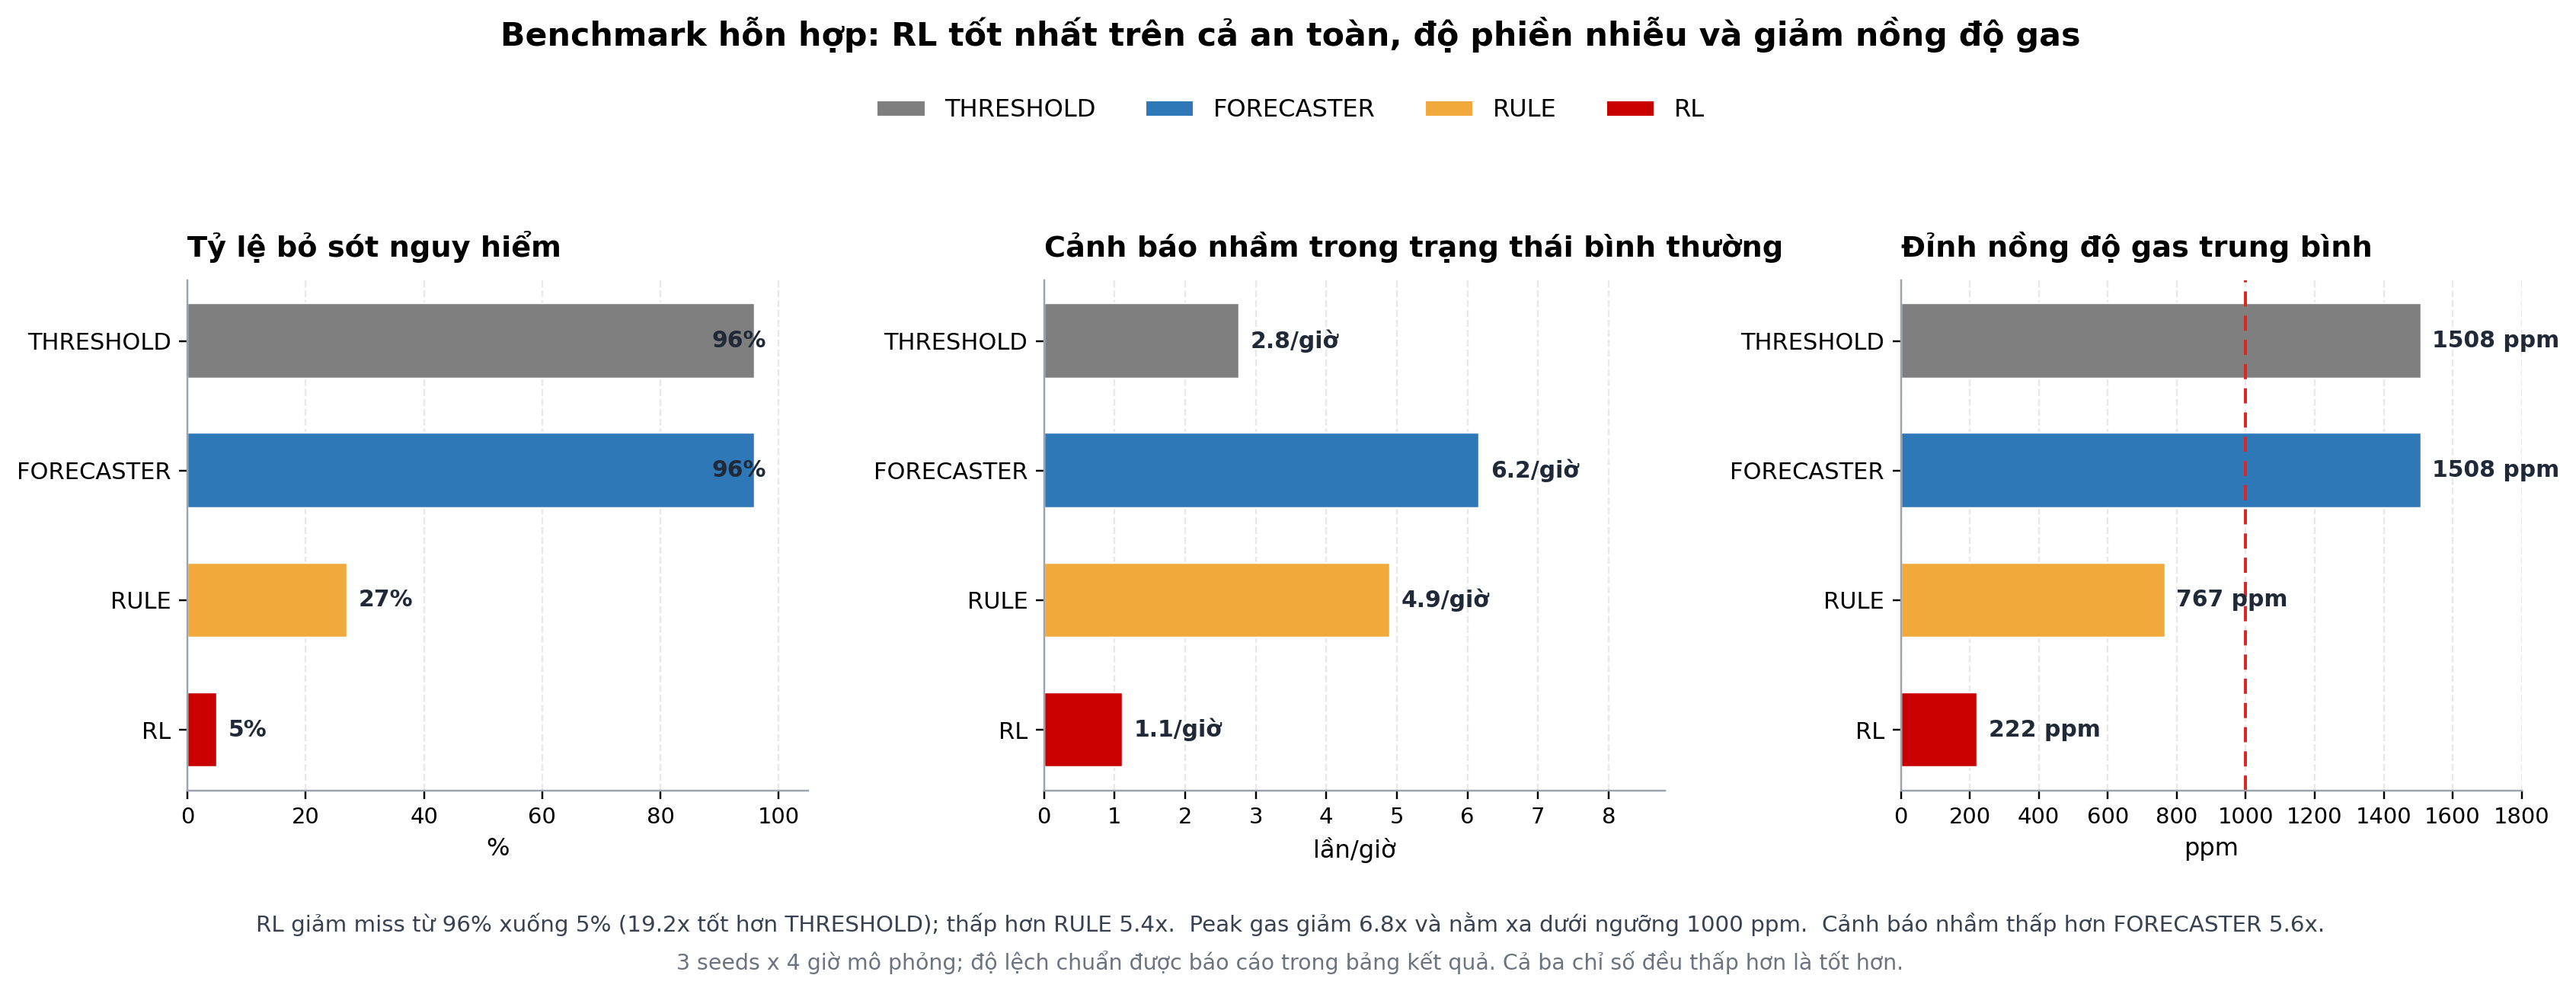
\includegraphics[width=\linewidth]{exp/benchmark_chart.png}
\captionof{figure}{So sánh bốn bộ điều khiển theo tỷ lệ bỏ sót, số cảnh báo mỗi giờ và nồng độ khí đỉnh.}
\label{fig:benchmark_chart}
\end{minipage}
\end{center}

\subsection{Đánh giá ablation trong benchmark: PPO-only và LSTM+PPO}

Để làm rõ vai trò của LSTM trong bộ điều khiển, đề tài bổ sung một thí nghiệm ablation giữa hai cấu hình \textbf{PPO-only} và \textbf{LSTM+PPO}. Ở cấu hình \textbf{LSTM+PPO}, hệ thống vận hành đúng pipeline hiện tại: LSTM sinh \texttt{predicted\_risk\_5min} và giá trị này được đưa vào PPO như chiều thứ năm của vector trạng thái 8 chiều. Ở cấu hình \textbf{PPO-only}, một tác nhân PPO riêng được huấn luyện lại với vector trạng thái 7 chiều, gồm \texttt{gas\_ppm}, nhiệt độ, độ ẩm, độ dốc nồng độ khí, trạng thái quạt, trạng thái van và thời gian từ hành động gần nhất; trường \texttt{predicted\_risk\_5min} không tồn tại trong đầu vào của mô hình. Như vậy, PPO-only không còn xét LSTM ở mức kiến trúc đầu vào, thay vì chỉ đặt giá trị LSTM bằng 0. Kết quả được so sánh nội bộ giữa hai cấu hình trên cùng seed và cùng kịch bản mô phỏng.

\begingroup
\small
\renewcommand{\arraystretch}{1.25}
\setlength{\tabcolsep}{5pt}
\setlength{\LTleft}{\fill}
\setlength{\LTright}{\fill}

\begin{longtable}{llcccc}
\caption{So sánh ablation giữa PPO-only và LSTM+PPO}
\label{tab:ppo_lstm_ablation} \\
\toprule
\textbf{Kịch bản} & \textbf{Cấu hình} & \textbf{Lead time} & \textbf{Miss rate} & \textbf{Peak gas} & \textbf{Chạm ngưỡng} \\
\midrule
\endfirsthead
\toprule
\textbf{Kịch bản} & \textbf{Cấu hình} & \textbf{Lead time} & \textbf{Miss rate} & \textbf{Peak gas} & \textbf{Chạm ngưỡng} \\
\midrule
\endhead
\endfoot
\bottomrule
\endlastfoot
TC-Slow & PPO-only  & $0{,}0 \pm 0{,}0$\,s     & $100{,}0$\% & $1{,}269 \pm 38$\,ppm & Có \\
        & LSTM+PPO  & $186{,}7 \pm 2{,}5$\,s   & $0{,}0$\%   & $74 \pm 20$\,ppm      & Không \\
\addlinespace
TC-Fast & PPO-only  & $0{,}0 \pm 0{,}0$\,s     & $100{,}0$\% & $2{,}000 \pm 0$\,ppm  & Có \\
        & LSTM+PPO  & $38{,}7 \pm 0{,}5$\,s    & $0{,}0$\%   & $97 \pm 53$\,ppm      & Không \\
\end{longtable}
\endgroup

Kết quả trong Bảng~\ref{tab:ppo_lstm_ablation} cho thấy khi không có tín hiệu \texttt{predicted\_risk\_5min} trong đầu vào, PPO-only không tạo được hành động kịp thời trong hai kịch bản rò rỉ được kiểm thử. \texttt{miss\_rate} đạt 100\%, nồng độ khí đỉnh vượt ngưỡng nguy hiểm ở cả TC-Slow và TC-Fast. Ngược lại, cấu hình LSTM+PPO phát hiện sớm hơn ngưỡng tới khoảng 187\,s trong rò rỉ chậm và khoảng 39\,s trong rò rỉ nhanh, đồng thời giữ nồng độ khí đỉnh dưới 100\,ppm trong trung bình ba seed. Điều này cho thấy các tín hiệu hiện tại như nồng độ khí và độ dốc có thể chưa đủ để PPO phản ứng sớm trong các kịch bản tăng nhanh; đầu ra dự báo của LSTM đóng vai trò cung cấp thông tin nhìn trước, giúp PPO chọn hành động trước khi khí vượt ngưỡng.

\begin{center}
\begin{minipage}{0.96\linewidth}
\centering
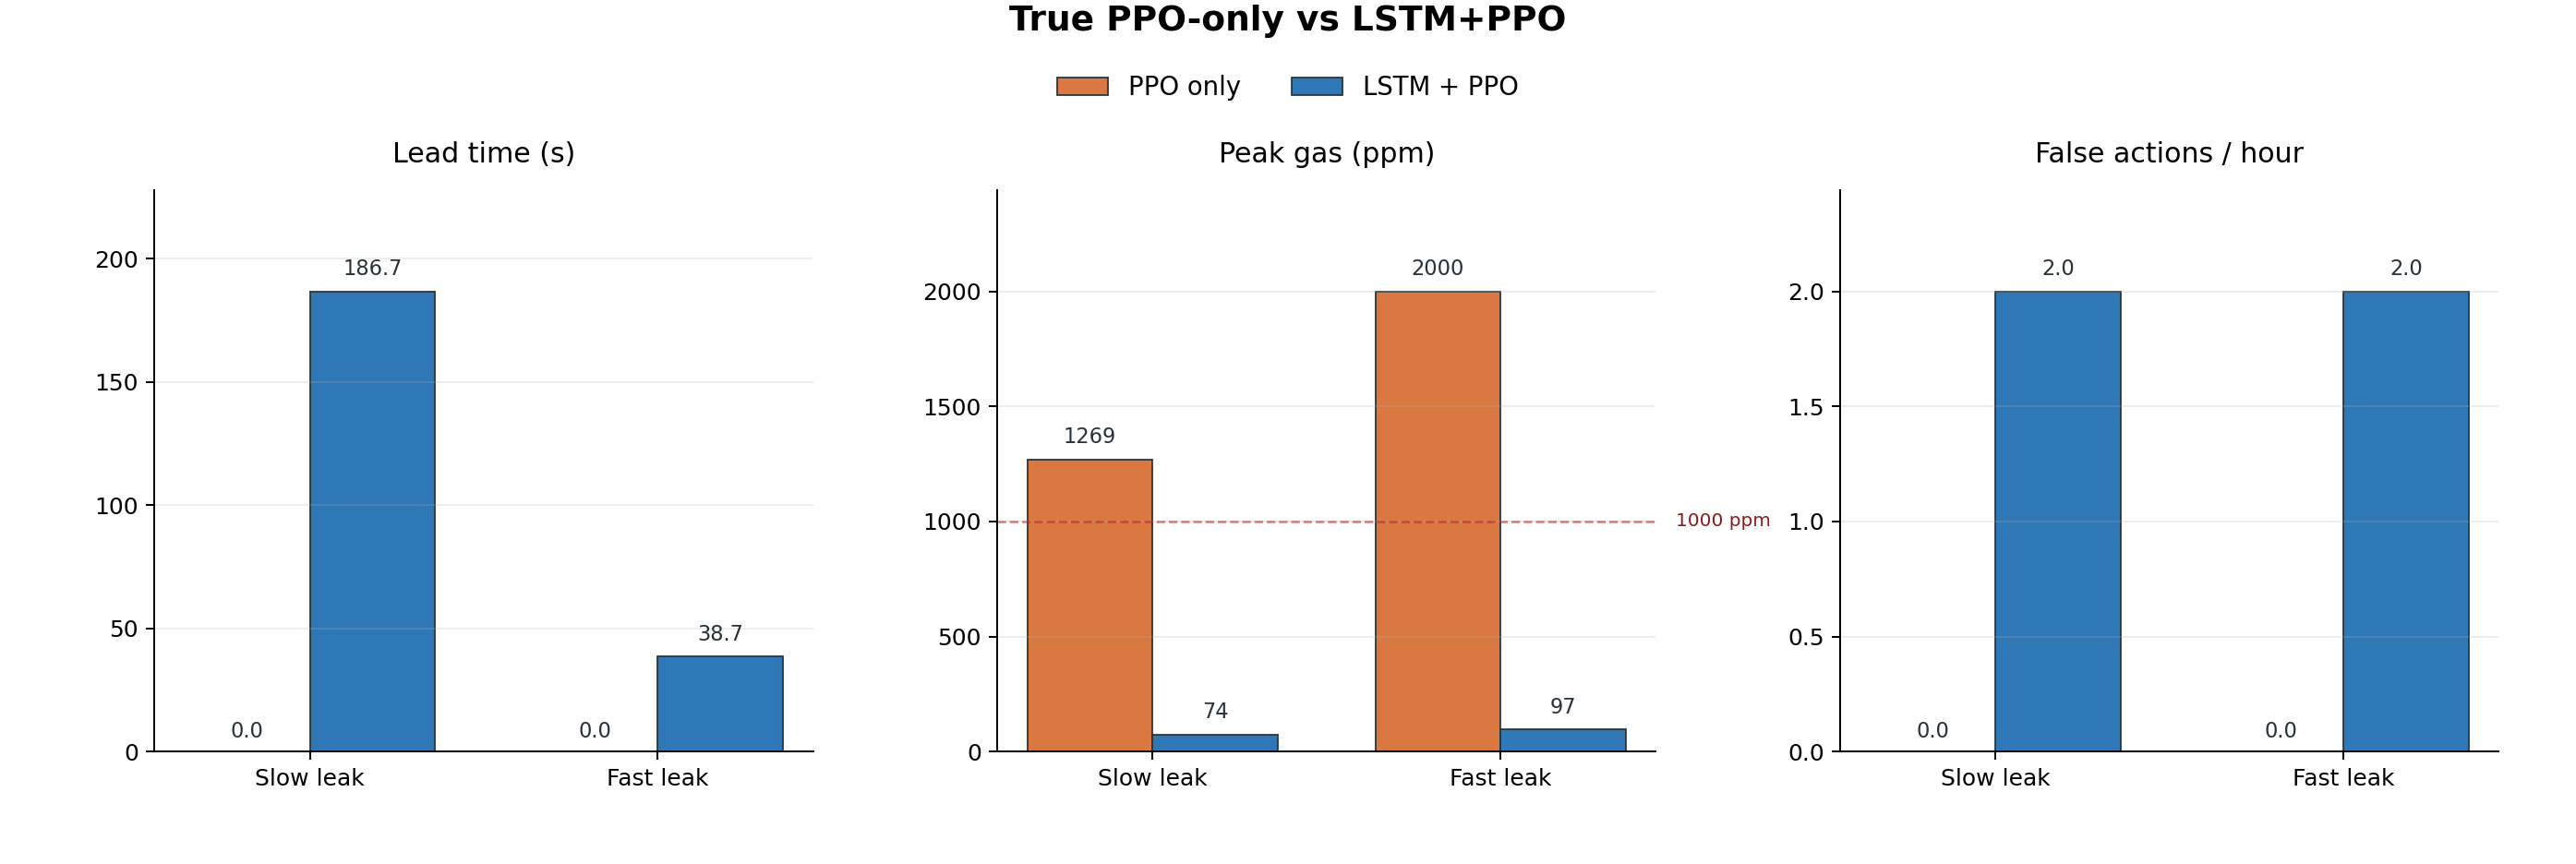
\includegraphics[width=\linewidth]{exp/ppo_lstm_ablation_chart.png}
\captionof{figure}{So sánh PPO-only 7 chiều và LSTM+PPO 8 chiều.}
\label{fig:ppo_lstm_ablation_chart}
\end{minipage}
\end{center}

\subsection{Kịch bản rò rỉ chậm và rò rỉ nhanh}

Để quan sát rõ hơn hành vi của từng bộ điều khiển, đề tài kiểm thử thêm hai kịch bản đơn: rò rỉ chậm và rò rỉ nhanh. TC-Slow là kịch bản rò rỉ chậm, trong đó khí tăng tuyến tính khoảng 5\,ppm/s và hệ thống có nhiều thời gian hơn để cảnh báo sớm. TC-Fast là kịch bản rò rỉ nhanh, trong đó khí tăng theo hàm mũ và yêu cầu hành động mạnh hơn. 

\begingroup
\small
\renewcommand{\arraystretch}{1.25}
\setlength{\tabcolsep}{6pt}
\setlength{\LTleft}{\fill}
\setlength{\LTright}{\fill}

\begin{longtable}{llccc}
\caption{Kết quả theo kịch bản rò rỉ chậm và rò rỉ nhanh}
\label{tab:scenarios_results} \\
\toprule
\textbf{Kịch bản} & \textbf{Controller} & \textbf{Lead time} & \textbf{Peak gas} & \textbf{Chạm ngưỡng} \\
\midrule
\endfirsthead
\toprule
\textbf{Kịch bản} & \textbf{Controller} & \textbf{Lead time} & \textbf{Peak gas} & \textbf{Chạm ngưỡng} \\
\midrule
\endhead
\endfoot
\bottomrule
\endlastfoot
TC-Slow & THRESHOLD  & 42\,s  & 1{,}500\,ppm & Có \\
        & FORECASTER & 182\,s & 1{,}500\,ppm & Có \\
        & RULE       & 185\,s & 142\,ppm     & Không \\
        & PPO        & 185\,s & 207\,ppm     & Không \\
\addlinespace
TC-Fast & THRESHOLD  & 4\,s   & 2{,}000\,ppm & Có \\
        & FORECASTER & 36\,s  & 2{,}000\,ppm & Có \\
        & RULE       & 38\,s  & 240\,ppm     & Không \\
        & PPO        & 38\,s  & 331\,ppm     & Không \\
\end{longtable}
\endgroup

Trong cả hai kịch bản, LSTM giúp tăng thời gian cảnh báo trước so với ngưỡng tĩnh. Tuy nhiên, nếu chỉ dùng FORECASTER thì hệ thống chỉ cảnh báo sớm, không làm giảm nồng độ khí. RULE và PPO giữ được khí dưới ngưỡng nhờ có hành động vật lý. Điều này cho thấy LSTM và PPO có vai trò bổ sung cho nhau: LSTM cung cấp tín hiệu dự báo, còn PPO quyết định hành động điều khiển.

\subsection{Testcase vận hành LSTM/PPO}
\label{sec:four_scenarios}

Hệ thống được kiểm thử qua bốn testcase thể hiện trên bảng điều khiển.

\begingroup
\footnotesize
\renewcommand{\arraystretch}{1.35}
\setlength{\tabcolsep}{5pt}
\setlength{\LTleft}{0pt}
\setlength{\LTright}{0pt}

\begin{longtable}{
  >{\raggedright\arraybackslash}p{2.8cm}
  >{\raggedright\arraybackslash}p{3.4cm}
  >{\raggedright\arraybackslash}p{\dimexpr\textwidth-6.2cm-6\tabcolsep\relax}
}
\caption{Bốn testcase vận hành dùng để kiểm chứng LSTM và PPO}
\label{tab:runtime_scenarios} \\
\toprule
\textbf{Testcase} 
& \textbf{Ngữ cảnh} 
& \textbf{Tiêu chí kiểm chứng} \\
\midrule
\endfirsthead
\toprule
\textbf{Testcase} 
& \textbf{Ngữ cảnh} 
& \textbf{Tiêu chí kiểm chứng} \\
\midrule
\endhead
\endfoot
\bottomrule
\endlastfoot

\makecell[l]{\texttt{TC1\_}\\\texttt{NORMAL}}
& Môi trường bình thường
& Không phát sinh cảnh báo sai; PPO giữ hành động \texttt{NO\_OP}; bảng điều khiển hiển thị ổn định. \\

\makecell[l]{\texttt{TC2\_}\\\texttt{COOKING}}
& Nấu ăn trong phòng kín
& Gas tăng có kiểm soát; LSTM phản ánh xu hướng tăng rủi ro; PPO cảnh báo hoặc bật quạt khi cần. \\

\makecell[l]{\texttt{TC3\_}\\\texttt{LEAK}}
& Rò rỉ tại dây dẫn hoặc khớp nối
& Risk tăng cao; PPO phản ứng bằng \texttt{FAN\_ON} hoặc \texttt{CLOSE\_VALVE}; cảnh báo được gửi đến người dùng. \\

\makecell[l]{\texttt{TC4\_}\\\texttt{RECOVERY}}
& Môi trường phục hồi sau điều khiển
& Gas giảm; hành động điều khiển giảm dần; tránh giữ quạt hoặc van ở trạng thái kích hoạt không cần thiết. \\

\end{longtable}
\endgroup

Các testcase được chạy bằng script \texttt{scripts/test/run-scenario.ps1}. Script thiết lập kịch bản mô phỏng, gán \texttt{device\_id} riêng cho từng testcase và gửi dữ liệu qua cùng luồng MQTT--Kafka--Spark như khi dùng thiết bị thật.

\begingroup
\footnotesize
\renewcommand{\arraystretch}{1.25}
\setlength{\tabcolsep}{5pt}
\setlength{\LTleft}{0pt}
\setlength{\LTright}{0pt}

\begin{longtable}{
  >{\raggedright\arraybackslash}p{1.7cm}
  >{\raggedright\arraybackslash}p{3.2cm}
  >{\raggedright\arraybackslash}p{\dimexpr\textwidth-6.9cm-8\tabcolsep\relax}
  >{\centering\arraybackslash}p{2.0cm}
}
\caption{Phân tích kết quả bốn testcase vận hành}
\label{tab:runtime_scenario_results} \\
\toprule
\textbf{Testcase} & \textbf{Kết quả kỳ vọng} & \textbf{Kết quả quan sát và ý nghĩa} & \textbf{Đánh giá} \\
\midrule
\endfirsthead
\toprule
\textbf{Testcase} & \textbf{Kết quả kỳ vọng} & \textbf{Kết quả quan sát và ý nghĩa} & \textbf{Đánh giá} \\
\midrule
\endhead
\endfoot
\bottomrule
\endlastfoot
TC1 & Gas thấp, risk thấp, không alert & Không có cảnh báo theo \texttt{device\_id}; gas dao động trong vùng bình thường; PPO không điều khiển thừa. & Đạt \\
TC2 & Gas tăng do nấu ăn/phòng kín & LSTM phản ánh xu hướng tăng qua \texttt{predicted\_risk\_5min}; PPO có thể cảnh báo hoặc bật quạt tùy mức gas. & Đạt có điều kiện \\
TC3 & Rò rỉ nguy hiểm, cần phản ứng mạnh & Khi gas/risk cao, PPO chuyển sang \texttt{FAN\_ON} hoặc \texttt{CLOSE\_VALVE}; alert feed và Telegram được kích hoạt. & Đạt \\
TC4 & Gas giảm sau điều khiển & Khi gas quay về vùng an toàn, PPO giảm hành động điều khiển, hạn chế giữ quạt/van không cần thiết. & Đạt \\
\end{longtable}
\endgroup

Bốn testcase này kiểm chứng hệ thống ở mức chức năng. TC1 cho thấy hệ thống không phản ứng bừa trong trạng thái bình thường. TC2 và TC3 cho thấy LSTM/PPO phản ứng theo xu hướng tăng và mức nguy hiểm của khí. TC4 cho thấy bộ điều khiển có xu hướng giảm can thiệp khi môi trường phục hồi.

\begin{center}
\begin{minipage}{0.92\linewidth}
\centering
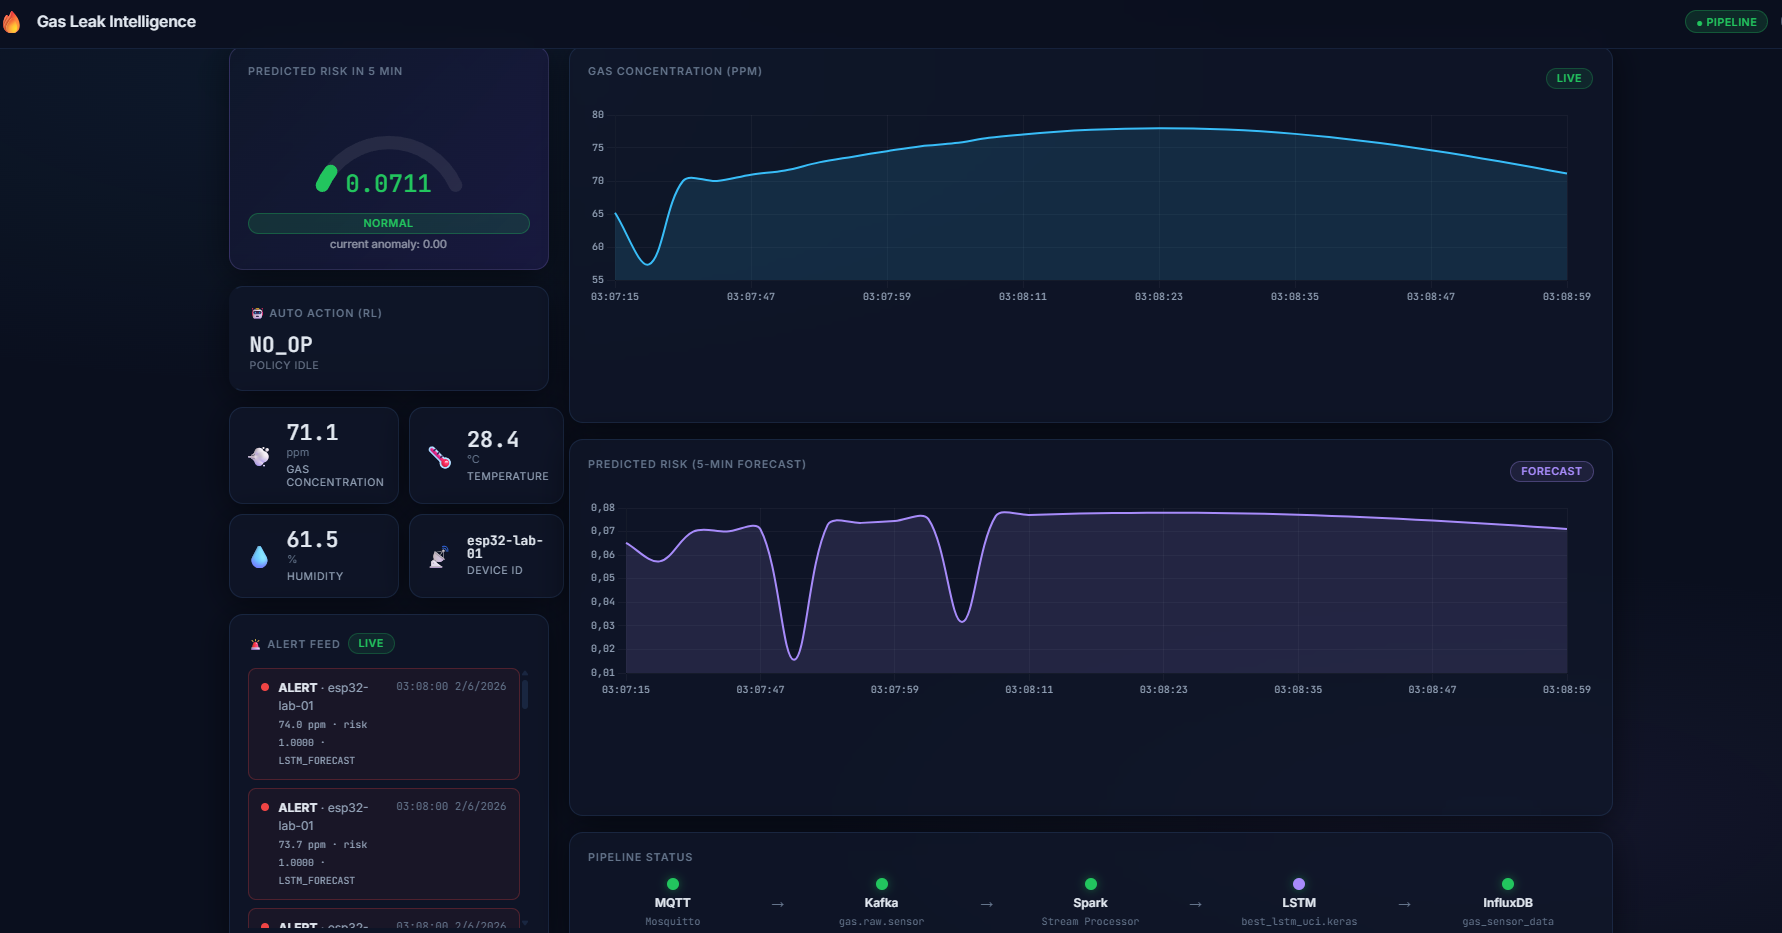
\includegraphics[width=\linewidth]{img/TC1.png}
\captionof{figure}{Kết quả bảng điều khiển của testcase TC1.}
\label{fig:tc1}
\end{minipage}
\end{center}

\begin{center}
\begin{minipage}{0.96\linewidth}
\centering
  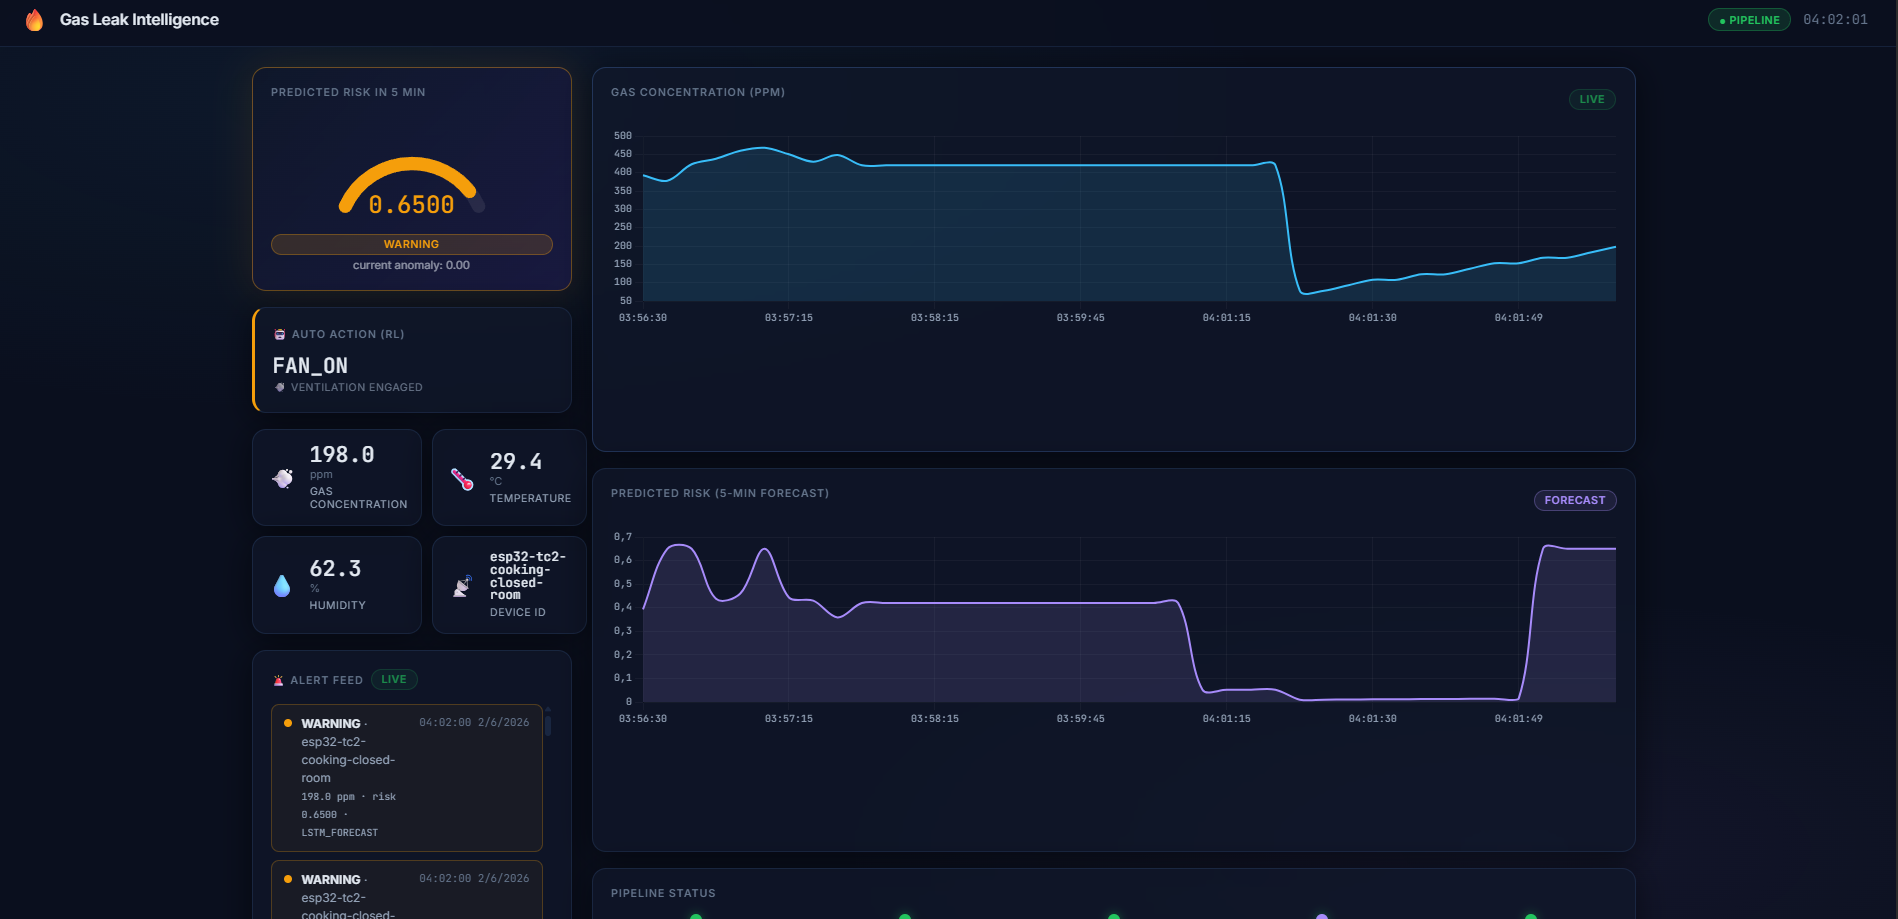
\includegraphics[width=0.48\linewidth]{img/TC2-1.png}
  \hfill
  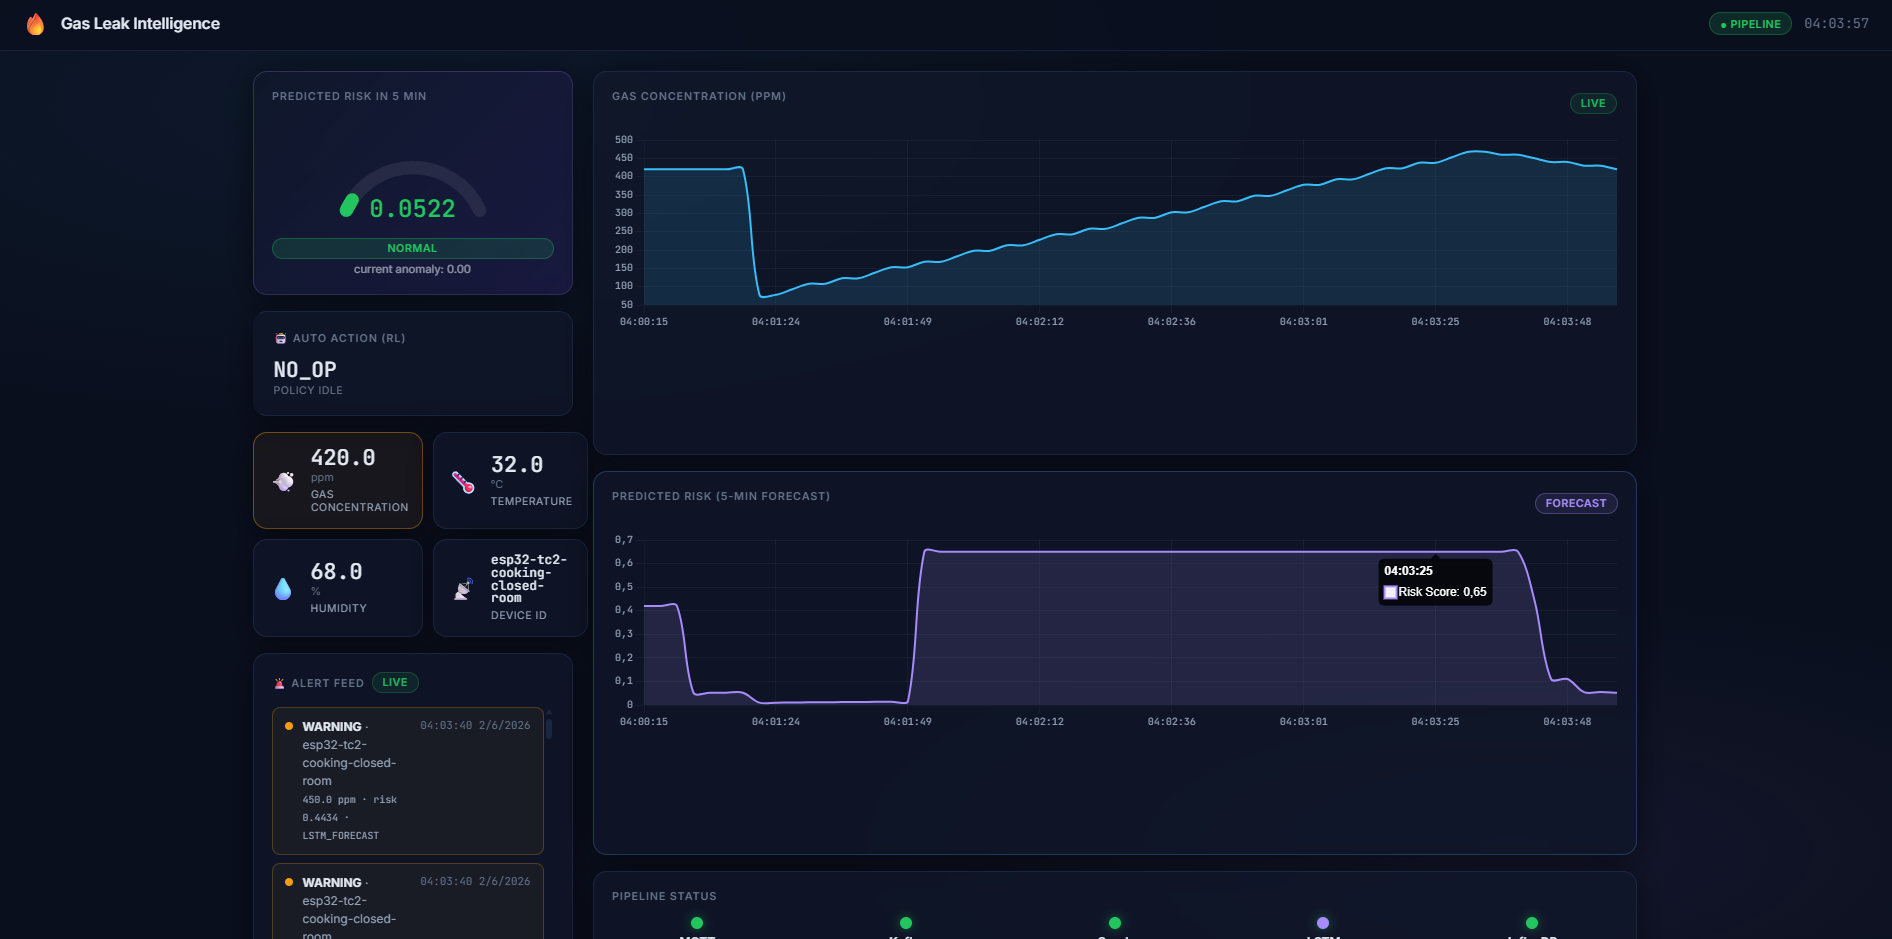
\includegraphics[width=0.48\linewidth]{img/TC2-2.png}

  \captionof{figure}{Kết quả bảng điều khiển của testcase TC2.}
  \label{fig:tc2_result}
\end{minipage}
\end{center}

\begin{center}
\begin{minipage}{0.96\linewidth}
\centering
  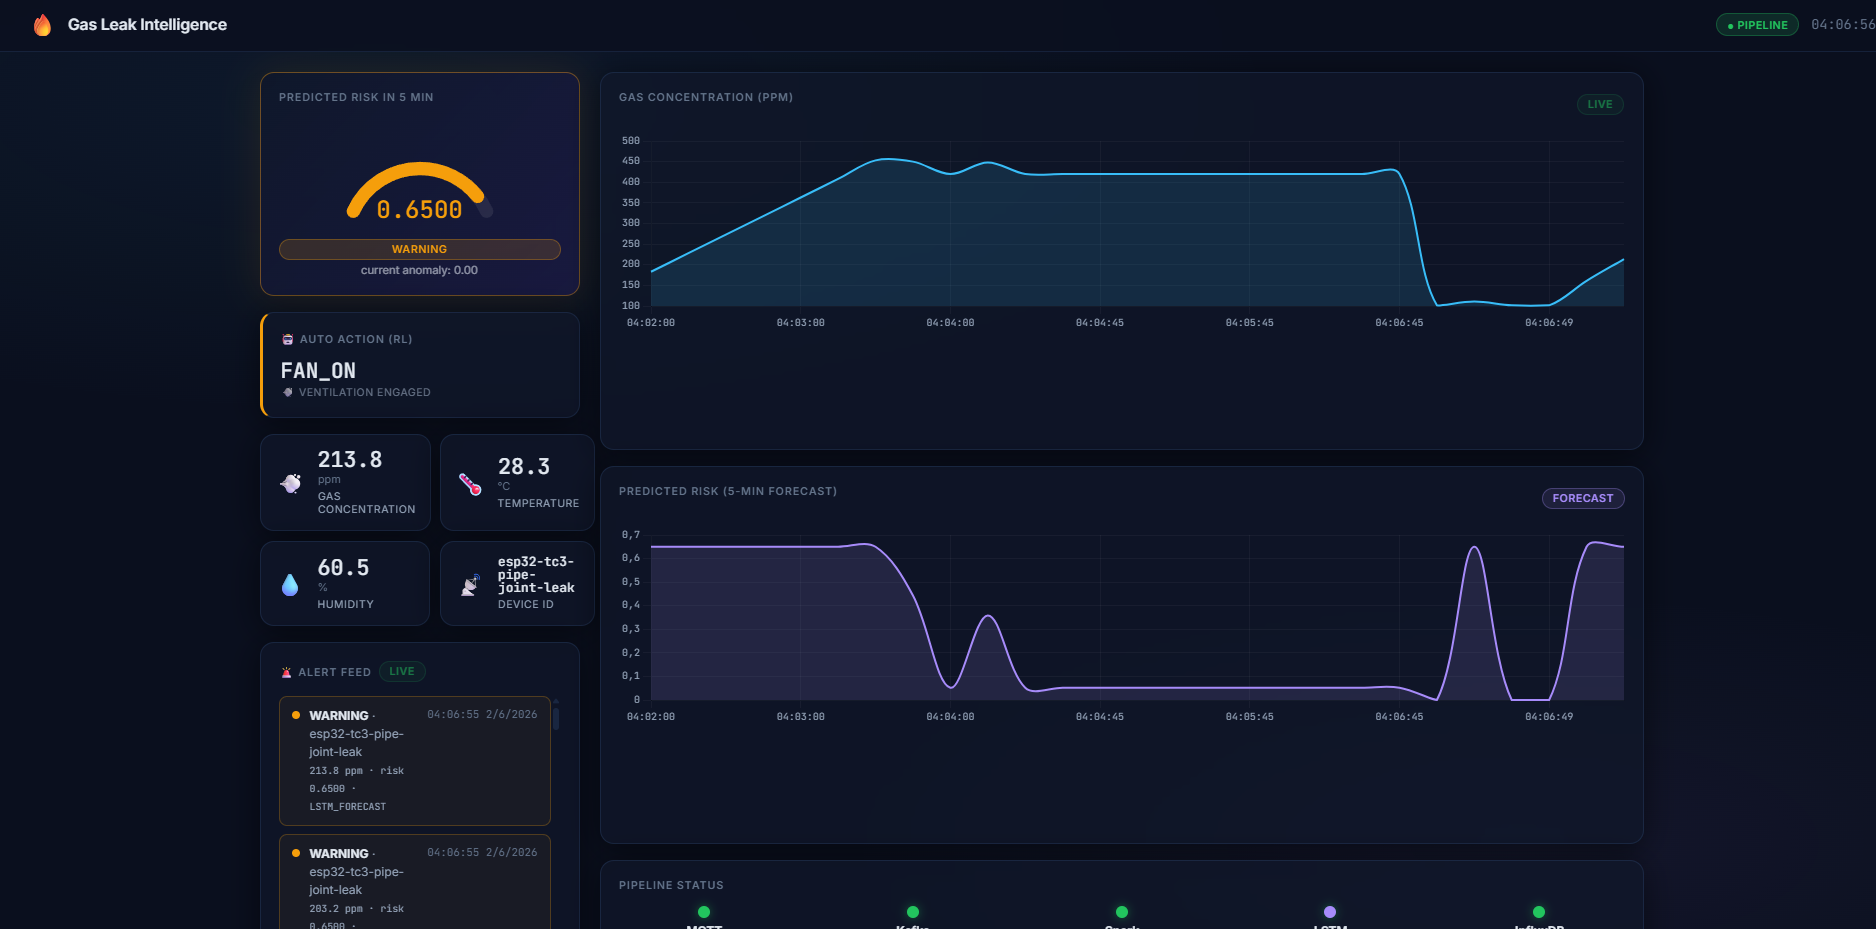
\includegraphics[width=0.48\linewidth]{img/TC3-1.png}
  \hfill
  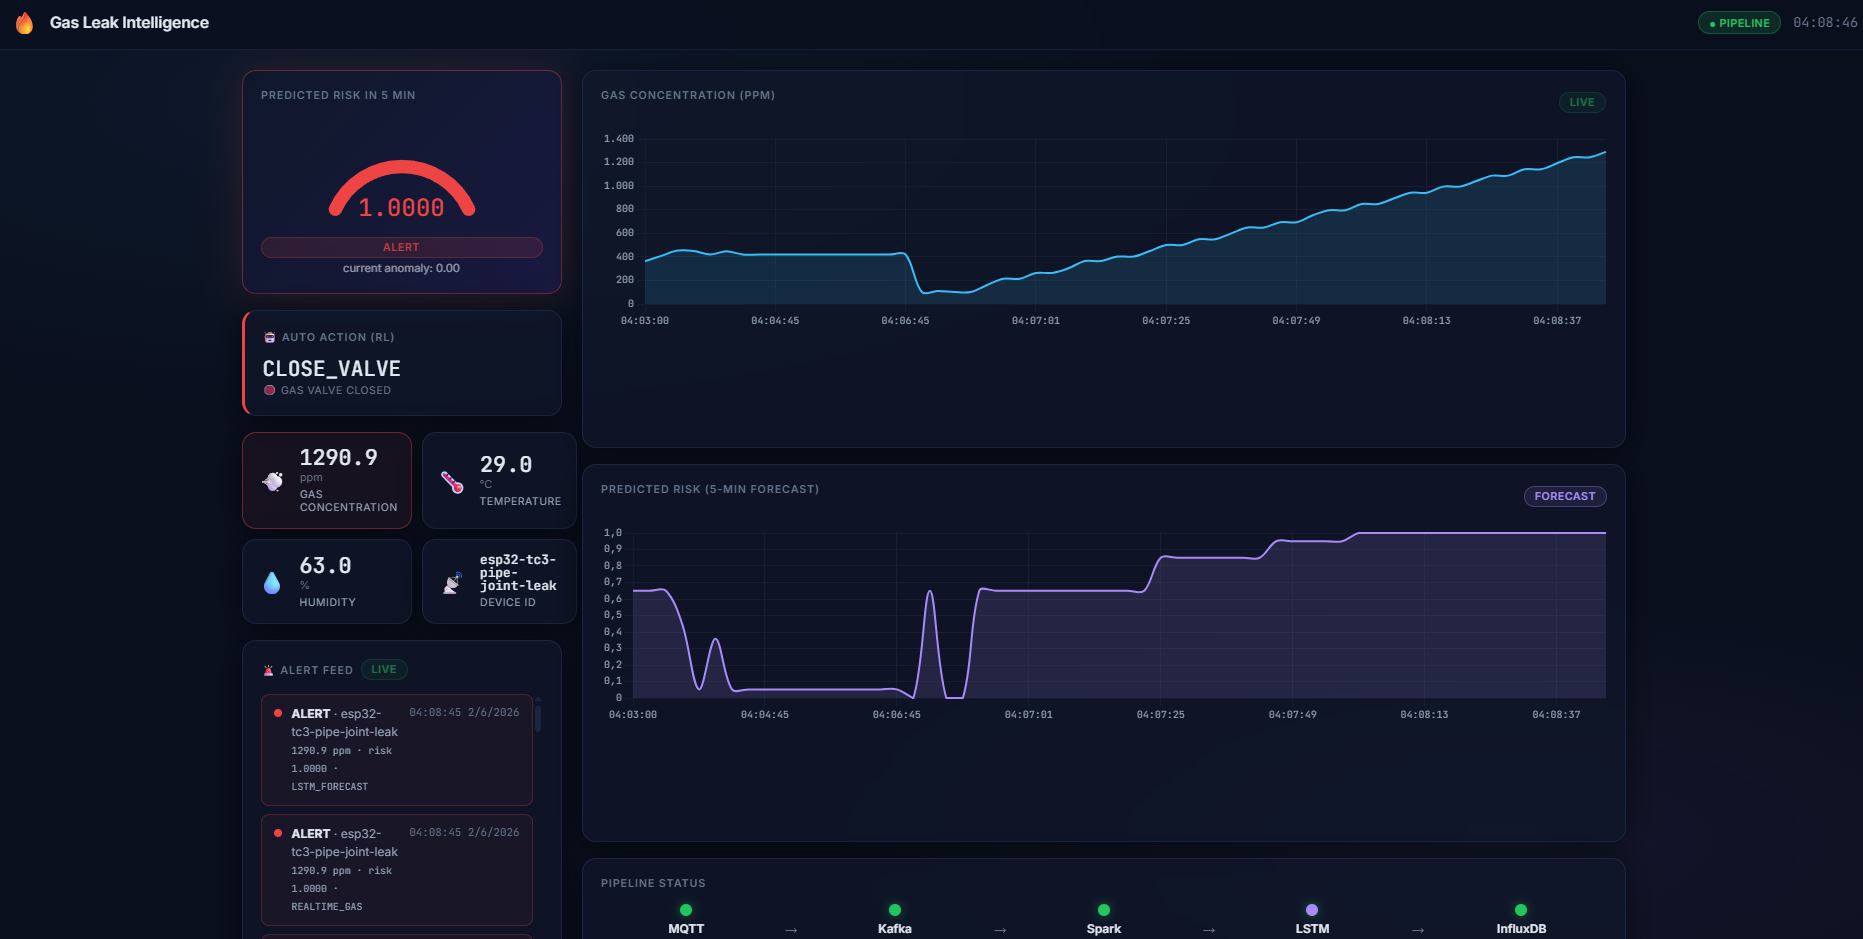
\includegraphics[width=0.48\linewidth]{img/TC3-2.png}

  \captionof{figure}{Kết quả bảng điều khiển của testcase TC3.}
  \label{fig:tc3_result}
\end{minipage}
\end{center}

\begin{center}
\begin{minipage}{0.42\linewidth}
\centering
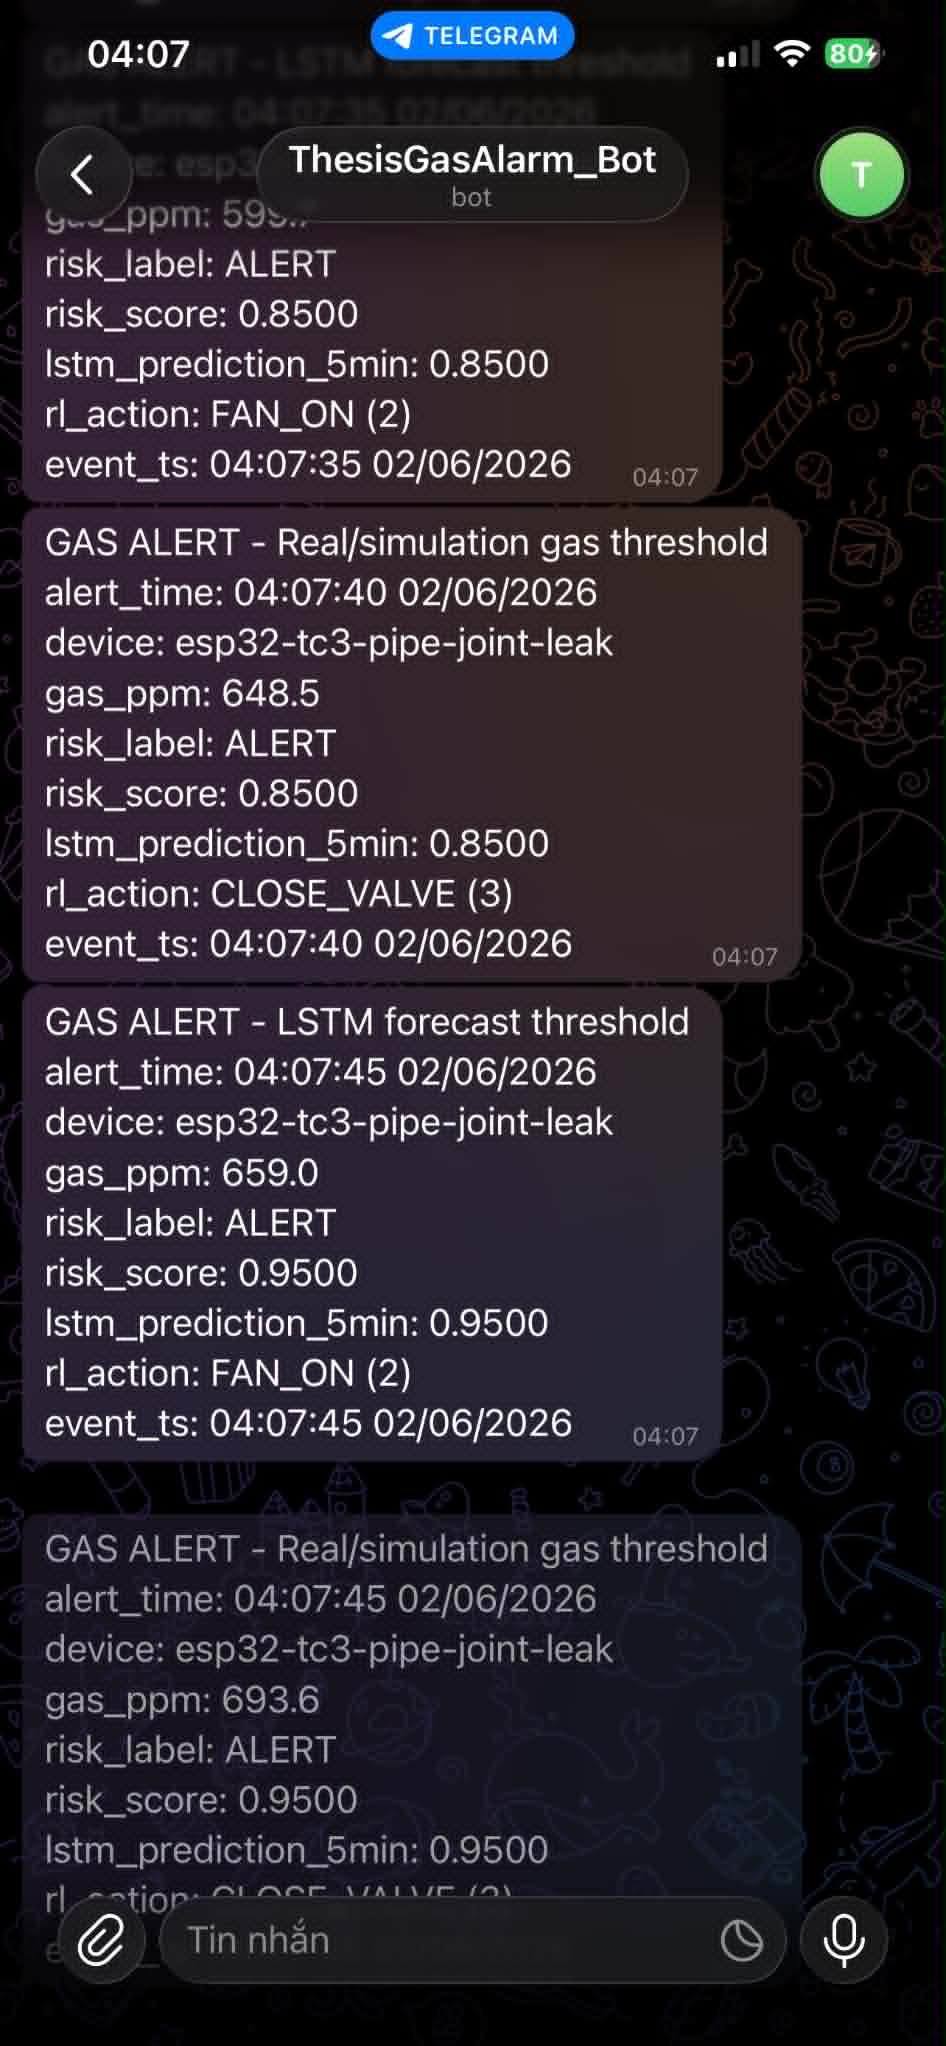
\includegraphics[width=0.82\linewidth]{img/tele_TC3.jpg}
\captionof{figure}{Thông báo Telegram trong testcase TC3.}
\label{fig:tele-tc3}
\end{minipage}
\end{center}

\begin{center}
\begin{minipage}{0.96\linewidth}
\centering
  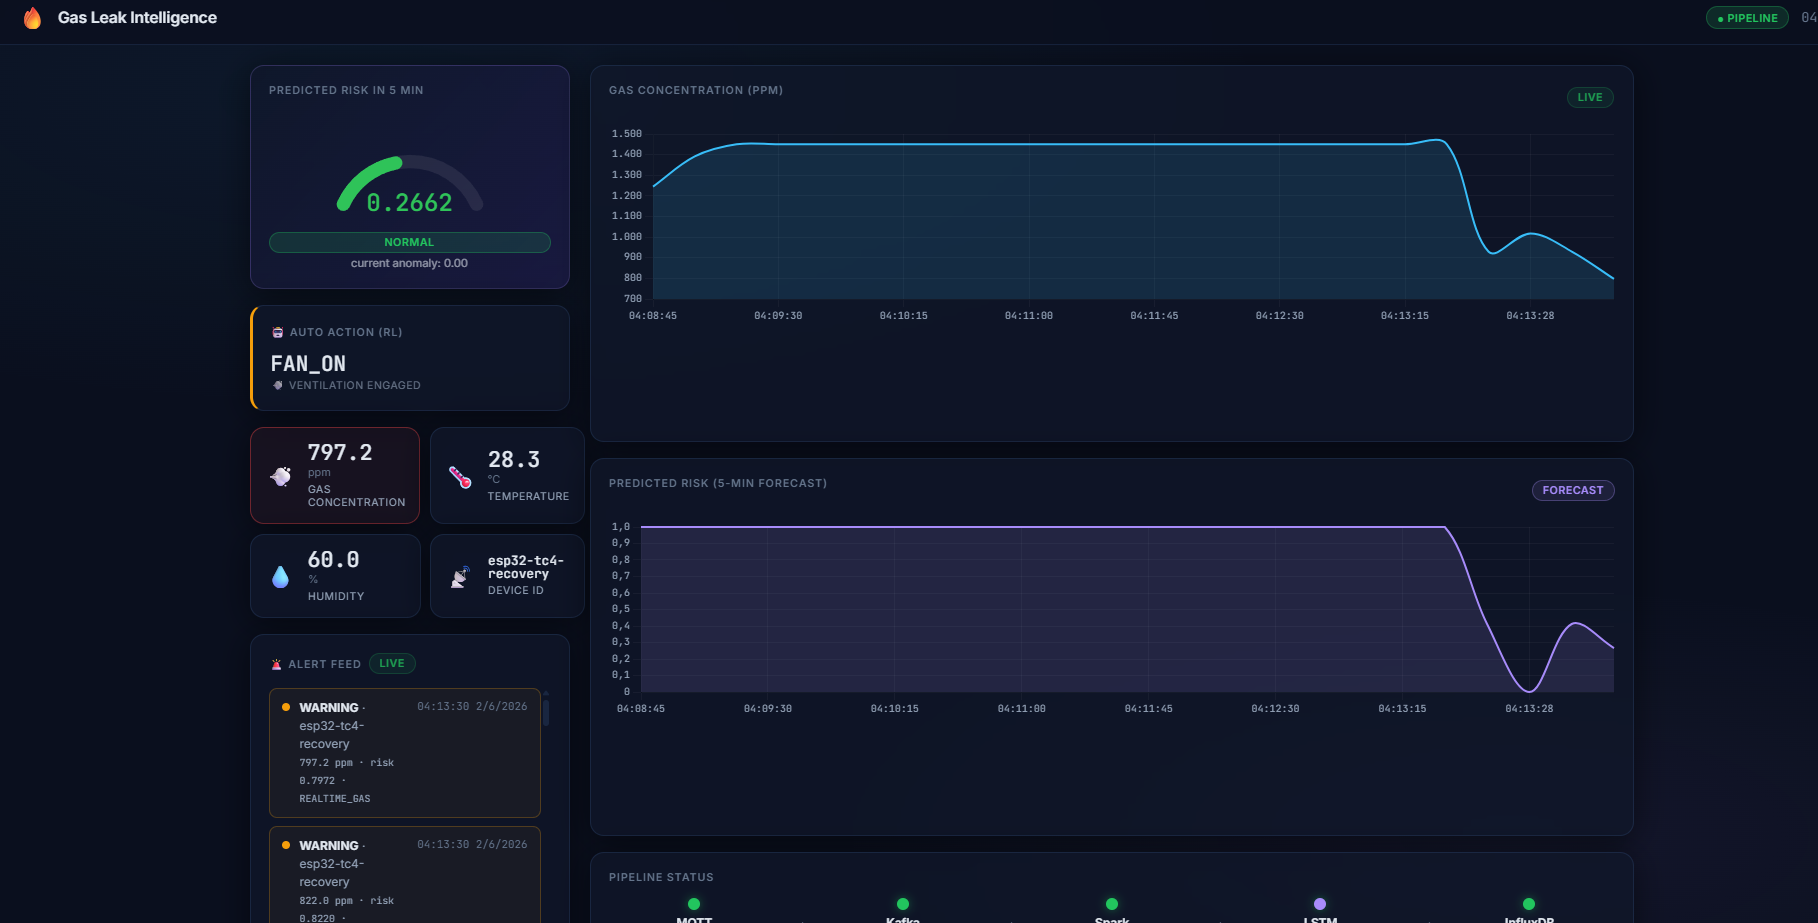
\includegraphics[width=0.48\linewidth]{img/TC4-1.png}
  \hfill
  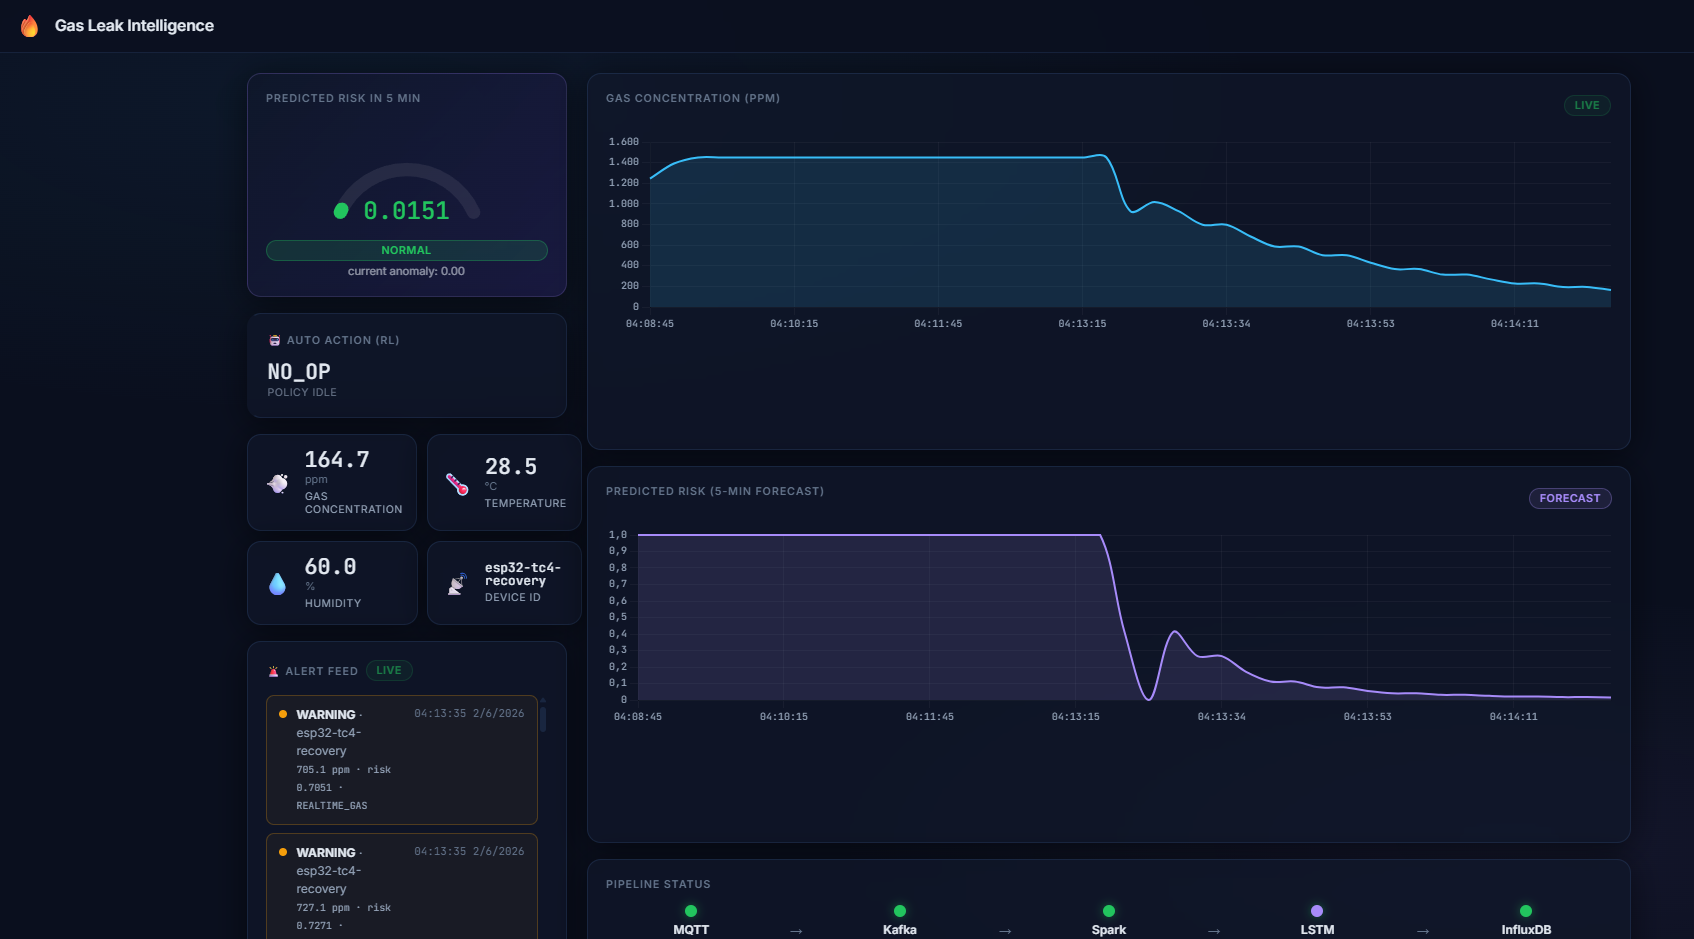
\includegraphics[width=0.48\linewidth]{img/TC4-2.png}

  \captionof{figure}{Kết quả bảng điều khiển của testcase TC4.}
  \label{fig:tc4_result}
\end{minipage}
\end{center}

\begin{center}
\begin{minipage}{0.42\linewidth}
\centering
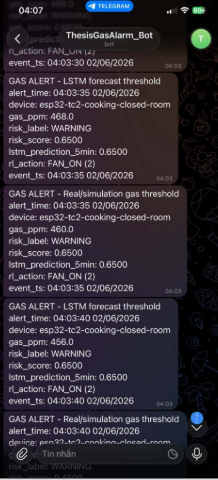
\includegraphics[width=0.82\linewidth]{img/tele-tc4.png}
\captionof{figure}{Thông báo Telegram trong testcase TC4.}
\label{fig:tele-tc4}
\end{minipage}
\end{center}

\subsection{Testcase luồng MQTT--Kafka--Spark}
\label{sec:kafka_pipeline_eval}

\noindent\textbf{a) Mục tiêu đánh giá}

Nhóm testcase luồng xử lý được xây dựng để kiểm tra việc dữ liệu có đi qua đầy đủ các thành phần MQTT, Kafka, Spark và InfluxDB hay không. Đồng thời, phần này cũng làm rõ vai trò của Kafka trong kiến trúc. Khi dữ liệu tăng nhanh hoặc xuất hiện đợt tăng đột biến, Kafka đóng vai trò bộ đệm, giúp tách tốc độ gửi dữ liệu của nguồn phát khỏi tốc độ xử lý của thành phần đọc.

\noindent\textbf{b) Kết quả testcase luồng xử lý}

Kết quả chạy script \texttt{scripts/test/run-kafka-pipeline-tests.ps1} được tổng hợp trong Bảng~\ref{tab:kafka_pipeline_results}.

\begingroup
\small
\renewcommand{\arraystretch}{1.25}
\setlength{\tabcolsep}{4pt}
\setlength{\LTleft}{0pt}
\setlength{\LTright}{0pt}

\begin{longtable}{
  >{\raggedright\arraybackslash}p{2.8cm}
  >{\raggedright\arraybackslash}p{3cm}
  >{\raggedright\arraybackslash}p{3cm}
  >{\raggedright\arraybackslash}p{\dimexpr\textwidth-8.8cm-8\tabcolsep\relax}
}
\caption{Kết quả testcase luồng MQTT--Kafka--Spark}
\label{tab:kafka_pipeline_results} \\
\toprule
\textbf{Testcase} & \textbf{Kafka} & \textbf{Spark/DB} & \textbf{Kết luận} \\
\midrule
\endfirsthead
\toprule
\textbf{Testcase} & \textbf{Kafka} & \textbf{Spark/DB} & \textbf{Kết luận} \\
\midrule
\endhead
\endfoot
\bottomrule
\endlastfoot
TC-P1 Basic & 60/60, 100\% & 60/60, 100\% & Pipeline cơ bản hoạt động đúng. \\
TC-P2 Tải trung bình & 500/500, 100\% & 500/500, 100\% & Ổn định ở tải trung bình, tốc độ gửi khoảng 41 msg/s. \\
TC-P3 Dữ liệu tăng đột biến & 1000/1000, 100\% & 1000/1000, 100\% & Kafka tiếp nhận đủ dữ liệu khi bản tin được gửi nhanh, tốc độ gửi khoảng 646 msg/s. \\
TC-P4 Multi-topic & Raw +5, Alert +6, Action +5 & 5/5 & Các topic raw, alert và action đều có dữ liệu. \\
TC-P5 Invalid data & Recovery 5/5 & Recovery 5/5 & Dữ liệu lỗi không làm bridge/Spark crash; hệ thống tiếp tục xử lý dữ liệu hợp lệ sau đó. \\
\end{longtable}
\endgroup

TC-P1 chứng minh luồng dữ liệu cơ bản hoạt động. TC-P2 cho thấy luồng xử lý vẫn ổn định ở tải trung bình. TC-P3 là testcase quan trọng để chứng minh vai trò bộ đệm của Kafka: dữ liệu được gửi nhanh nhưng Kafka vẫn tiếp nhận đủ bản tin và Spark xử lý dần theo micro-batch. TC-P5 cho thấy hệ thống có khả năng phục hồi khi gặp dữ liệu lỗi.

\begin{center}
\begin{minipage}{0.86\linewidth}
\centering
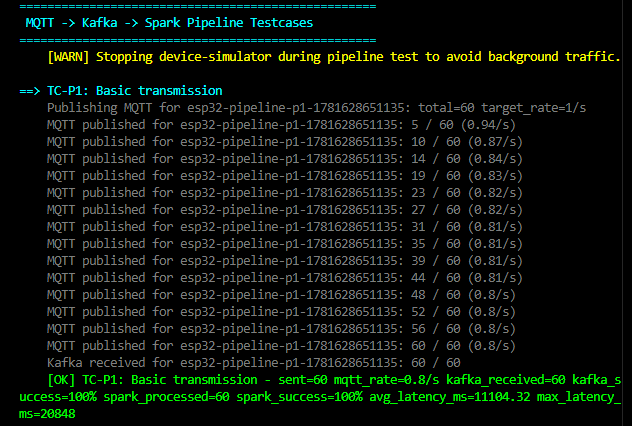
\includegraphics[width=\linewidth]{img/TC-P1.png}
\captionof{figure}{Kết quả kiểm thử luồng xử lý TC-P1.}
\label{fig:TC-P1}
\end{minipage}
\end{center}

\begin{center}
\begin{minipage}{0.86\linewidth}
\centering
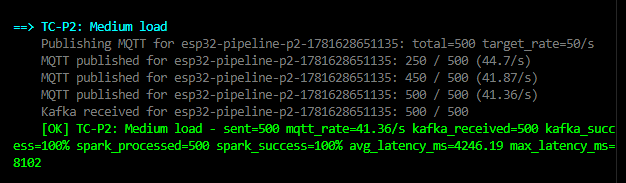
\includegraphics[width=\linewidth]{img/TC-P2.png}
\captionof{figure}{Kết quả kiểm thử luồng xử lý TC-P2.}
\label{fig:TC-P2}
\end{minipage}
\end{center}

\begin{center}
\begin{minipage}{0.86\linewidth}
\centering
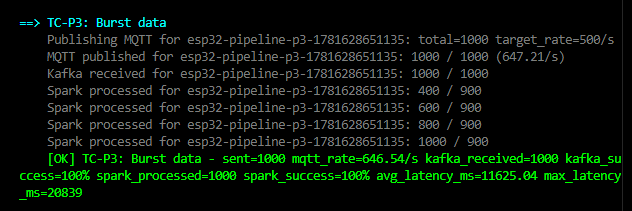
\includegraphics[width=\linewidth]{img/TC-P3.png}
\captionof{figure}{Kết quả kiểm thử luồng xử lý TC-P3.}
\label{fig:TC-P3}
\end{minipage}
\end{center}

\begin{center}
\begin{minipage}{0.86\linewidth}
\centering
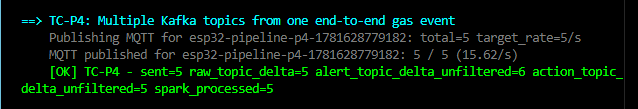
\includegraphics[width=\linewidth]{img/TC-P4.png}
\captionof{figure}{Kết quả kiểm thử luồng xử lý TC-P4.}
\label{fig:TC-P4}
\end{minipage}
\end{center}

\begin{center}
\begin{minipage}{0.86\linewidth}
\centering
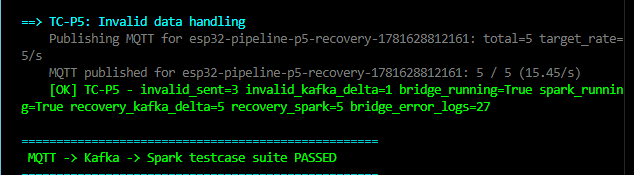
\includegraphics[width=\linewidth]{img/TC-P5.png}
\captionof{figure}{Kết quả kiểm thử luồng xử lý TC-P5.}
\label{fig:TC-P5}
\end{minipage}
\end{center}

\subsection{Độ trễ suy luận LSTM/PPO}
\label{sec:model_latency_eval}

Ngoài độ trễ của luồng xử lý, đề tài đo riêng thời gian suy luận của bộ dự báo LSTM và tác nhân PPO. Kết quả được trình bày trong Bảng~\ref{tab:latency_model}. Trong đó, Mean là độ trễ trung bình, Median là trung vị, P95 là mức mà 95\% mẫu đo nhỏ hơn hoặc bằng giá trị này, và P99 là mức mà 99\% mẫu đo nhỏ hơn hoặc bằng giá trị này. P95/P99 giúp quan sát độ trễ ở phần đuôi phân phối, quan trọng hơn trung bình khi đánh giá hệ thống thời gian thực mềm.

\begingroup
\small
\renewcommand{\arraystretch}{1.25}
\setlength{\tabcolsep}{4pt}
\setlength{\LTleft}{\fill}
\setlength{\LTright}{\fill}

\begin{longtable}{lcccc}
\caption{Độ trễ suy luận mô hình}
\label{tab:latency_model} \\
\toprule
\textbf{Thành phần} & \textbf{Mean} & \textbf{Median} & \textbf{P95} & \textbf{P99} \\
\midrule
\endfirsthead
\toprule
\textbf{Thành phần} & \textbf{Mean} & \textbf{Median} & \textbf{P95} & \textbf{P99} \\
\midrule
\endhead
\endfoot
\bottomrule
\endlastfoot
LSTM bộ dự báo & 76{,}333 ms & 71{,}113 ms & 113{,}650 ms & 136{,}310 ms \\
PPO choose action & 0{,}703 ms & 0{,}690 ms & 0{,}813 ms & 0{,}943 ms \\
\end{longtable}
\endgroup

Kết quả cho thấy LSTM là thành phần tốn thời gian hơn, nhưng độ trễ vài chục mili-giây vẫn nhỏ so với chu kỳ lấy mẫu ở mức giây. PPO gần như không phải nút thắt vì thời gian chọn hành động dưới 1 ms. Vì vậy, độ trễ đầu cuối chủ yếu đến từ micro-batch, I/O và quá trình ghi/đọc cơ sở dữ liệu, không phải từ bộ điều khiển PPO.

\vspace{0.5em}
\noindent\textbf{Kết chương.}

Kết quả đánh giá hệ thống thể hiện qua: mô hình LSTM, bộ điều khiển PPO và luồng triển khai. Kết quả LSTM cho thấy mô hình có khả năng học xu hướng rủi ro từ chuỗi cảm biến theo dạng dự báo sự kiện trong tương lai. Kết quả PPO cho thấy bộ điều khiển có thể giảm \texttt{miss\_rate}, giảm \texttt{peak\_gas} và hạn chế cảnh báo sai tốt hơn các đường cơ sở trong môi trường mô phỏng.

Nhóm testcase kiểm tra kết quả LSTM và PPO TC1--TC4 cho thấy hệ thống phản ứng hợp lý trong các trạng thái bình thường, tăng rủi ro, rò rỉ nguy hiểm và phục hồi. Nhóm testcase luồng xử lý TC-P1--TC-P5 cho thấy Kafka có vai trò rõ ràng trong việc tiếp nhận, đệm và chuyển tiếp dữ liệu cho Spark xử lý. Tóm lại, hệ thống đáp ứng mục tiêu của khóa luận ở mức mô phỏng và tích hợp phần mềm: dữ liệu được xử lý theo thời gian thực, LSTM cung cấp tín hiệu dự báo, PPO lựa chọn hành động điều khiển, còn bảng điều khiển và Telegram hỗ trợ hiển thị/cảnh báo cho người dùng.


\chapter{Kết luận và hướng phát triển}
\label{c:ketluanvaphattrien}
% ============================================================
%  Chương 5: Kết luận và hướng phát triển
% ============================================================

Chương này tổng hợp các kết quả đã đạt được, chỉ ra những hạn chế còn tồn tại và đề xuất hướng phát triển tiếp theo. Các kết luận được đặt trong phạm vi mô phỏng và kiểm thử phần mềm đã trình bày ở Chương~\ref{c:thucnghiemdanhgia}; hệ thống chưa được xem là một sản phẩm an toàn hoàn chỉnh nếu chưa kiểm thử với phần cứng và điều kiện khí gas thực tế.

\section{Kết luận}

Khóa luận này đã trình bày việc thiết kế, triển khai và đánh giá một nền tảng IoT 4 lớp cho phát hiện và ứng phó rò rỉ khí gas. So với hướng cảnh báo bằng ngưỡng tĩnh, đề tài đạt được một số kết quả chính sau:

\subsection{Những kết quả đạt được}

\begin{enumerate}
  \item Mô hình LSTM dự báo: Chuyển từ bài toán gán nhãn trạng thái hiện tại sang bài toán dự báo xác suất rủi ro trong 5 phút tới. Mô hình được huấn luyện trên dữ liệu tổng hợp từ bộ mô phỏng và được kiểm chứng bổ sung trên dữ liệu cảm biến IoT công khai từ Kaggle (Accuracy 96{,}4\%, Recall 92{,}8\%). Kết quả này mới dừng ở mức tham khảo vì nhãn trên dữ liệu thực là nhãn proxy, nhưng giúp nhóm có thêm cơ sở để đánh giá khả năng học xu hướng tín hiệu của kiến trúc LSTM ngoài dữ liệu mô phỏng. Cơ chế dự phòng bằng ngoại suy xu hướng cũng được thêm vào để hệ thống vẫn có dự báo cơ bản khi chưa tải được mô hình.

  \item Bộ điều khiển PPO: Học chính sách trong môi trường Gymnasium tích hợp bộ mô phỏng, với khả năng lựa chọn bốn hành động (NO\_OP/ALERT/FAN\_ON/CLOSE\_VALVE). Với hàm thưởng dựa trên kết quả kiềm chế khí (đã loại bỏ hiện tượng khai thác sai hàm thưởng của phiên bản đầu), bộ điều khiển PPO cho kết quả tốt trong đánh giá so sánh mô phỏng: tỷ lệ bỏ sót 5\% (luật tay 27\%, ngưỡng tĩnh 96\%), nồng độ đỉnh trung bình 222\,ppm (đường cơ sở 1{,}508\,ppm), và số cảnh báo sai 1{,}1/giờ. Điểm đáng chú ý là chính sách được học từ tương tác với môi trường thay vì viết sẵn toàn bộ bằng các ngưỡng if--else.

  \item Luồng xử lý dữ liệu: Kiến trúc MQTT $\rightarrow$ Kafka $\rightarrow$ Spark cho phép xử lý dữ liệu cảm biến gần thời gian thực với độ trễ đầu cuối dưới 350 ms trong cấu hình thử nghiệm, đồng thời vẫn có hướng mở rộng khi số thiết bị tăng.

  \item Tích hợp Telegram chatbot: Cung cấp kênh cảnh báo đẩy, truy vấn trạng thái và quản lý đăng ký nhận thông báo mà không cần cài ứng dụng riêng.

  \item Phương pháp đánh giá: Định nghĩa \texttt{miss} theo \emph{kết quả} (khí có thực sự chạm 1000\,ppm hay không), phù hợp cho cả bộ điều khiển chỉ cảnh báo và bộ điều khiển có làm thay đổi quỹ đạo vật lý. Ngoài ra, đề tài bổ sung đường cơ sở luật tay (\texttt{RULE}) để so sánh với PPO trên các chỉ số thời gian cảnh báo trước, tỷ lệ bỏ sót, nồng độ khí đỉnh và cảnh báo sai.

  \item Triển khai Docker Compose: Toàn bộ hệ thống 10 dịch vụ có thể khởi động bằng một lệnh duy nhất, giúp việc demo và kiểm tra lại kết quả thuận tiện hơn.
\end{enumerate}

\subsection{Hạn chế}

\begin{itemize}
  \item Kết quả chính vẫn dựa trên dữ liệu mô phỏng: Khi chưa có phần cứng và dữ liệu thực đầy đủ, dữ liệu mô phỏng là nguồn dữ liệu chính. Vì vậy, nếu mô phỏng còn đơn giản thì mô hình học được cũng khó phản ánh đầy đủ các đặc tính như nhiễu cảm biến, trôi tín hiệu, vị trí đặt cảm biến và điều kiện thông gió thật.

  \item Dữ liệu Kaggle chỉ có nhãn proxy: Tập dữ liệu cảm biến IoT công khai không cung cấp nhãn rò rỉ LPG thật, nên nhãn dương được xây dựng theo phân vị cao của tín hiệu LPG. Vì vậy, kết quả trên Kaggle chỉ chứng minh sơ bộ khả năng học xu hướng tín hiệu, chưa chứng minh độ an toàn trong môi trường gas thực.

  \item Bộ điều khiển PPO chưa được kiểm thử trên phần cứng: Agent hiện học trong môi trường mô phỏng, nơi hành động đóng van hoặc bật quạt có tác động lý tưởng hóa. Khi triển khai thực, cần kiểm tra độ trễ cơ cấu chấp hành, sai số cảm biến và các ràng buộc an toàn vật lý.

  \item Số seed và kịch bản benchmark còn hạn chế: Benchmark hiện đã so sánh bốn bộ điều khiển và hai kịch bản rò rỉ chậm/rò rỉ nhanh, nhưng vẫn cần nhiều seed, nhiều cấu hình phòng và nhiều kiểu nhiễu hơn để kết luận chắc hơn về độ ổn định của chính sách.

\end{itemize}

\section{Hướng phát triển}

Đề tài có thể được phát triển theo các hướng sau:

\begin{itemize}
  \item \textbf{Triển khai và kiểm thử trên phần cứng thực:} Thay thế bộ mô phỏng bằng ESP32 kết hợp cảm biến MQ và DHT22 trong môi trường phòng thí nghiệm có kiểm soát. Hướng này giúp đánh giá hệ thống trên dữ liệu cảm biến thực, bao gồm nhiễu, độ trôi tín hiệu và độ trễ khi vận hành.

  \item \textbf{Cải thiện mô hình dự báo và điều khiển:} Thử nghiệm các mô hình chuỗi thời gian nâng cao hơn như Transformer-based time series hoặc Temporal Fusion Transformer để so sánh với LSTM. Đồng thời, tinh chỉnh PPO trên dữ liệu thực nhằm giảm khoảng cách giữa mô phỏng và triển khai thực tế.

  \item \textbf{Mở rộng khả năng ứng dụng:} Hỗ trợ nhiều thiết bị cảm biến trong cùng không gian để phát hiện vị trí rò rỉ, kết hợp thêm cảm biến đa loại hoặc camera hồng ngoại để nhận diện loại khí và dấu hiệu cháy, hướng đến chuẩn hóa hệ thống cho môi trường dân dụng hoặc công nghiệp.
\end{itemize}

\section{Tổng kết}

Đề tài đã xây dựng được một nguyên mẫu có thể chạy lại để khảo sát việc áp dụng LSTM và PPO vào bài toán phát hiện, ứng phó rò rỉ khí gas. Kiến trúc 4 lớp kết hợp bộ mô phỏng, Docker Compose, Telegram bot và bảng điều khiển thời gian thực.

Trong benchmark mô phỏng hiện tại, cách tiếp cận kết hợp LSTM + PPO đạt kết quả tốt hơn ngưỡng tĩnh và luật tay trên các chỉ số được đo (bỏ sót 5\% so với 27--96\%, peak gas 222\,ppm so với tối đa 1{,}508\,ppm). Tuy nhiên, đây vẫn là kết quả trên môi trường mô phỏng. Để có thể kết luận chắc hơn về triển khai an toàn, hệ thống cần được kiểm thử tiếp với nhiều seed, nhiều kịch bản và phần cứng cảm biến thực.


\begingroup
\setlength{\emergencystretch}{8em}
\phantomsection
\addcontentsline{toc}{chapter}{Tài liệu tham khảo}

\nocite{*}

\printbibheading[title={Tài liệu tham khảo}]
\justifying
\printbibliography[heading=subbibliography, title={Tài liệu tiếng Việt}, category=vietnamese]
\printbibliography[heading=subbibliography, title={Tài liệu tiếng Anh}, notcategory=vietnamese]
\endgroup

\end{document}
